\documentclass[11pt,oneside]{book}
\usepackage{fontspec}
\setmainfont{Noto Serif}
\setsansfont{Noto Sans}
\setmonofont{Noto Sans Mono}
\newfontfamily\proseunicodefont{DejaVu Serif}
\usepackage[margin=1in]{geometry}
\usepackage{microtype}
\usepackage{amsmath,amssymb,amsthm,mathtools,bm}
\usepackage{graphicx}
\usepackage{xcolor}
\usepackage{booktabs}
\usepackage{array}
\usepackage{longtable}
\usepackage{enumitem}
\usepackage{float}
\usepackage{caption}
\usepackage{hyperref}
\usepackage{fancyhdr}
\usepackage{tikz}
\usetikzlibrary{arrows.meta,positioning,calc,decorations.pathmorphing}

\hypersetup{
  colorlinks=true,
  linkcolor=blue!50!black,
  urlcolor=blue!50!black,
  citecolor=blue!50!black
}

\setlength{\parskip}{0.5em}
\setlength{\parindent}{0pt}
\setlist[itemize]{topsep=0.25em,itemsep=0.2em}
\setlist[enumerate]{topsep=0.25em,itemsep=0.2em}
\setlength{\headheight}{40pt}
\numberwithin{equation}{chapter}

\newtheorem{theorem}{نظرية}[chapter]
\newtheorem{proposition}[theorem]{قضية}
\newtheorem{lemma}[theorem]{لمّة}
\newtheorem{corollary}[theorem]{نتيجة}
\theoremstyle{definition}
\newtheorem{definition}[theorem]{تعريف}
\newtheorem{example}[theorem]{مثال}
\theoremstyle{remark}
\newtheorem{remark}[theorem]{ملاحظة}

\providecommand{\ket}[1]{\left\lvert#1\right\rangle}
\providecommand{\bra}[1]{\left\langle#1\right\rvert}
\providecommand{\braket}[2]{\left\langle#1\,\middle|\,#2\right\rangle}
\providecommand{\expect}[1]{\left\langle#1\right\rangle}
\newcommand{\lectureoverview}[1]{\paragraph{نظرة عامة.} #1}
\newenvironment{classroomqa}{%
  \par\medskip
  \begin{minipage}{0.96\textwidth}
}{%
  \end{minipage}
  \par\medskip
}
\newcommand{\audiencequestion}[1]{\noindent\textbf{سؤال من الحضور.} #1\par\smallskip}
\newcommand{\lecturerresponse}[1]{\noindent\textbf{الإجابة.} #1\par}
\newcommand{\lecturetimestamp}[1]{\footnote{التوقيت في المحاضرة: #1.}}
\newcommand{\lectureframe}[1]{\par\smallskip{\centering\footnotesize\itshape لقطة المحاضرة: #1.\par}}
\newcommand{\editorialnote}[1]{\footnote{توضيح تحريري: #1}}

\makeatletter
\newcommand{\course@headerfont}{\normalfont\small\itshape}
\newcommand{\course@pagefont}{\normalfont\small}
\newcommand{\course@headerraise}{14pt}
\newlength{\course@headerboxheight}
\setlength{\course@headerboxheight}{\dimexpr\headheight-\course@headerraise-9pt\relax}
\newcommand{\course@leftheadbox}[1]{%
  \raisebox{\course@headerraise}{%
    \parbox[t][\course@headerboxheight][t]{0.82\textwidth}{%
      \raggedright\course@headerfont\strut\MakeUppercase{#1}\strut%
    }%
  }%
}
\newcommand{\course@rightheadbox}[1]{%
  \raisebox{\course@headerraise}{%
    \parbox[t][\course@headerboxheight][t]{0.82\textwidth}{%
      \raggedleft\course@headerfont\strut\MakeUppercase{#1}\strut%
    }%
  }%
}
\renewcommand{\chaptermark}[1]{\markboth{\MakeUppercase{\chaptername\ \thechapter.\ #1}}{}}
\renewcommand{\sectionmark}[1]{\markright{\MakeUppercase{\thesection\hspace{0.4em}#1}}}
\fancyhf{}
\fancyhead[L]{\course@leftheadbox{\leftmark}}
\fancyhead[R]{\course@pagefont\thepage}
\renewcommand{\headrulewidth}{0.5pt}
\pagestyle{fancy}
\fancypagestyle{plain}{%
  \fancyhf{}
  \fancyhead[L]{\course@leftheadbox{\leftmark}}
  \fancyhead[R]{\course@pagefont\thepage}
  \renewcommand{\headrulewidth}{0.5pt}
}
\makeatother

\usepackage{polyglossia}
\setdefaultlanguage{arabic}
\usepackage{sectsty}
\setotherlanguage{english}
\newfontfamily\arabicfont[Script=Arabic]{Amiri}
\newfontfamily\arabicfontsf[Script=Arabic]{Amiri}
\newfontfamily\arabicfonttt[Script=Arabic]{DejaVu Sans Mono}
\let\arabicsectionnumber\thesection
\let\arabicsubsectionnumber\thesubsection
\renewcommand{\thesection}{\LRE{\arabicsectionnumber}}
\renewcommand{\thesubsection}{\LRE{\arabicsubsectionnumber}}
\renewcommand{\contentsname}{المحتويات}
\renewcommand{\chaptername}{الفصل}
\renewcommand{\figurename}{الشكل}
\renewcommand{\tablename}{الجدول}
\renewcommand{\proofname}{البرهان}
\renewcommand{\bibname}{المراجع}
\sectionfont{\raggedleft}
\subsectionfont{\raggedleft}
\makeatletter
\renewcommand{\@pnumwidth}{2.2em}
\renewcommand{\@tocrmarg}{3.2em}
\makeatother
\usepackage{tocloft}
\renewcommand{\cftchapfont}{\small\bfseries}
\renewcommand{\cftchappagefont}{\small\bfseries}
\renewcommand{\cftsecfont}{\small}
\renewcommand{\cftsecpagefont}{\small}
\setlength{\cftsecnumwidth}{3em}
\renewcommand{\cftsubsecfont}{\small}
\renewcommand{\cftsubsecpagefont}{\small}
\setlength{\cftsubsecindent}{4.5em}
\setlength{\cftsubsecnumwidth}{4em}
\emergencystretch=6em
\pdfstringdefDisableCommands{\def\proseunicodefont{}}

\geometry{paperwidth=177.6mm,paperheight=252mm,left=16mm,right=16mm,
 top=18mm,bottom=18mm,includeheadfoot,headheight=28pt,headsep=7mm,footskip=9mm}
\usepackage{scrextend}
\changefontsizes[17pt]{12pt}
\raggedbottom
\renewenvironment{classroomqa}{\par\medskip\begingroup}{\par\endgroup\medskip}
\fancyhf{}
\setlength{\headwidth}{\textwidth}
\fancyhead[L]{\parbox{\textwidth}{\raggedleft\fontsize{9}{11}\selectfont\nouppercase{\leftmark}}}
\fancyfoot[C]{\small\thepage}
\renewcommand{\headrulewidth}{0.3pt}
\fancypagestyle{plain}{\fancyhf{}\fancyfoot[C]{\small\thepage}\renewcommand{\headrulewidth}{0pt}}

\hypersetup{
  pdftitle={Quantum Entanglement, Part 3},
  pdfauthor={Lectures by Leonard Susskind; companion edition by LazyingArt LLC},
  pdfsubject={Independently edited companion notes for the 2006 Fall lecture course},
  pdfcreator={LaTeX with hyperref}
}
\graphicspath{{../../../generated_course_notes/supplementary/quantum_entanglement/2006_fall_part_3/figures/}{../../../generated_course_notes/supplementary/quantum_entanglement/2006_fall_part_3/assets/}}
\begin{document}
\frontmatter
\hypersetup{pageanchor=false}
\begin{titlepage}
\hyphenpenalty=10000\exhyphenpenalty=10000
\thispagestyle{empty}
\begin{tikzpicture}[remember picture,overlay]
  \node[anchor=center,inner sep=0] at (current page.center) {%
    \includegraphics[height=\paperheight,keepaspectratio]{../../../generated_course_notes/supplementary/quantum_entanglement/2006_fall_part_3/assets/cover-art.png}%
  };
  \node[
    anchor=north west,
    align=right,
    text width=0.78\paperwidth,
    fill=white,
    fill opacity=0.9,
    rounded corners=8pt,
    inner xsep=10pt,
    inner ysep=8pt
  ] at ([xshift=0.08\paperwidth,yshift=-0.06\paperheight]current page.north west) {%
    {\fontsize{30}{33}\selectfont\bfseries\color{black!88} \RLE{التشابك الكمي: الجزء الثالث}\\[0.85em]}
    {\large\color{black!72} \RLE{النسخة العربية / خريف 2006، الجزء الثالث}}
  };
  \node[
    anchor=south west,
    align=right,
    text width=0.68\paperwidth,
    fill=white,
    fill opacity=0.82,
    text opacity=1,
    rounded corners=6pt,
    inner sep=12pt
  ] at ([xshift=0.08\paperwidth,yshift=0.08\paperheight]current page.south west) {%
    {\normalsize\color{black!78} \RLE{المحاضرات الأصلية: \LRE{Leonard Susskind}}\\[0.35em]}
    {\small\color{black!72} \RLE{النسخة المصاحبة: \LRE{\href{https://lazying.art}{LazyingArt LLC} / \href{https://github.com/lachlanchen/Video2Book}{Video2Book}}}}
  };
\end{tikzpicture}
\mbox{}
\end{titlepage}
\hypersetup{pageanchor=true}

\clearpage
\chapter*{حول هذه الملاحظات}
تتبع هذه الملاحظات المرافقة، التي حُرِّرت بصورة مستقلة، الجزء الثالث من سلسلة محاضرات ليونارد سسكايند لعام 2006 عن التشابك الكمي. وقد أُعيد بناؤها استنادًا إلى التفريغات الآلية، والترجمات النصية، ولقطات مختارة للسبورة، ثم جرى التحقق منها بالرجوع إلى المادة المصدرية المتاحة. وهي ليست مخطوطة أصلية للأستاذ سسكايند، ولم يراجعها أو يعتمدها.

أُعِدَّت هذه الطبعة من قِبل \href{https://lazying.art}{LazyingArt LLC} باستخدام مجموعة الأدوات مفتوحة المصدر \href{https://github.com/lachlanchen/Video2Book}{Video2Book}. ولا تزال التفريغات الآلية متاحةً بصورة منفصلة، وقد تحتوي على أخطاء في التعرّف. ويُشار في الحواشي السفلية إلى الإيضاحات التحريرية وعمليات إعادة البناء غير البسيطة.
\clearpage
\tableofcontents
\mainmatter
\chapter{النسبية الخاصة: الأطر المرجعية، والتزامن، وتحويل لورنتز}

النسبية هي المبدأ القائل إن قوانين الفيزياء لا تعتمد على أي إطار قصوري نستخدمه لوصفها. ومهمتنا الأولى هي الحركيات: معنى المكان والزمان والحركة والمزامنة، والتحويل من إطار قصوري إلى آخر. أما الديناميكا فتأتي بعد ذلك، مع الطاقة النسبية، والزخم، والقوة، والنظير لمعادلة نيوتن للحركة، ومعنى \(E=mc^2\). وبمجرد أن يترسخ هذا البناء، يمكننا أن نقترب من النسبية العامة من الناحية المفاهيمية عبر الزمكان المنحني، وحركة الجسيمات في مجال ثقالي محدد سلفًا، والثقوب السوداء، وتمدد الكون، من غير أن نبدأ بالمشكلة الصعبة المتمثلة في حل معادلات حقل أينشتاين.

يجدر بنا أن نميز بين الصرامة المفاهيمية والصرامة الرياضية. لن نستخدم تقريبًا نعلم سلفًا أنه خاطئ. بل سنؤكد ما يفعله المجال الثقالي بالساعات والجسيمات والهندسة، مع إرجاء الأدوات اللازمة لبناء حلول اعتباطية لمعادلات الحقل. ويجب تناول النسبية الخاصة بمزيد من التصريح، لأن كل ذلك الاستدلال اللاحق يرتكز على حركياتها.

ولذلك فالموضع الصحيح للبدء ليس بمعادلة ذائعة الصيت، بل بعرض دقيق لما يعنيه الراصد بمكان وزمان.

\section{الإطار هو نظام إحداثيات فيزيائي}

تخيّل الفضاء مملوءًا بشبكة من مساطر مترية يمكن جعلها دقيقة بقدر ما نشاء. وتُعطى كل نقطة في الشبكة ثلاثة إحداثيات مكانية، وعند كل نقطة ساعة. وتكوّن القضبان والساعات معًا إطارًا مرجعيًا.

\begin{definition}
ال\emph{حدث} هو شيء يقع في مكان واحد وزمان واحد. في بُعد مكاني واحد تُكتب إحداثياته \((x,t)\)؛ وفي ثلاثة أبعاد تكون \((x,y,z,t)\).
\end{definition}

تضيف الفيزياء النيوتنية افتراضًا قويًا: يمكن مزامنة جميع الساعات المثالية مرة واحدة وإلى الأبد. الزمن كوني. قد تُنقل ساعة، وقد يحمل الراصد ساعة يد، لكن من المفترض أن يتفق الجميع على القيمة نفسها لـ \(t\) في كل مكان. ويُسمى هذا أحيانًا الزمن المطلق؛ ويمكن تصوره على أنه زمن الله، ساعة واحدة للعالم كله.

مبدأ النسبية أقدم من أينشتاين. وصورته الطبيعية هي قطار يتحرك بانتظام شديد فوق قضبان ملساء تمامًا بحيث لا شيء يقرع أو يهتز. وداخل القطار يمكننا أن نقذف الكرات ونلتقطها تمامًا كما نفعل في قطار واقف عند المحطة. إن التلاعب بالكرات تجربة صغيرة في الميكانيكا مكتملة على نحو يبعث على الدهشة: فهي تتطلب التوقيت، والجاذبية، والمحاذاة، والتحكم المتكرر في المسارات. وإذا كان القطار يتحرك بسرعة ثابتة، فلا تتغير أي من تلك القواعد. فالكرة المقذوفة مباشرة إلى أعلى تعود إلى اليد نفسها؛ ولا ينزلق القطار مبتعدًا من تحتها. وقد أدرك غاليليو هذه الحقيقة، وصاغها نيوتن على نحو منهجي في قوانين الحركة.

قبل غاليليو، كان من المغري أن نستدل بأن القطار المتحرك ينبغي أن يتقدم بينما تكون الكرة في الهواء، مما يضطر اللاعب إلى أن يمد يده إلى الخلف أو إلى الأمام ليستعيدها. والخطأ هو نسيان أن الكرة تشارك القطار بالفعل سرعته الأفقية حين تغادر اليد. ولا تكشف أي تجربة محصورة داخل العربة المتحركة بسلاسة عن حالة مميزة من السكون المطلق. إنما الحركة النسبية بين القطارين وحدها هي القابلة للرصد.

وعليه، فالقطار الساكن والقطار المتحرك حركة منتظمة هما إطاران قصوريان. وقبل أينشتاين، كانت العلاقة بينهما تُعطى بتحويلات غاليليو.

\section{رسم الزمكان}

نهمل \(y\) و\(z\) في الوقت الحاضر، ونرسم الزمن رأسيًا والموضع \(x\) أفقيًا. كل نقطة في الرسم تمثل حدثًا. والخط \(x=0\) هو تاريخ أصل المكان، أو \emph{خط العالم} الخاص به. أما الخطوط الرأسية المجاورة \(x=1,2,3,\ldots\) فهي خطوط العالم لنقاط الشبكة الأخرى. والخطوط الأفقية هي مجموعات من الأحداث ذات زمن مشترك.

\begin{figure}[H]
\centering
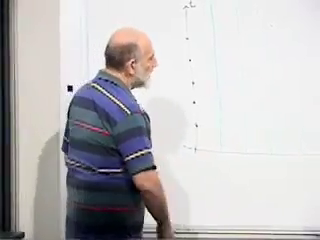
\includegraphics[width=0.62\textwidth]{lecture_01_figure_02.png}
\caption{محور الزمن في إطار السكون وأولى خطوط العالم للشبكة المكانية.}
\lectureframe{00:16:38}
\end{figure}

ويظهر البناء نفسه بوضوح أكبر في رسم مثالي:

\begin{figure}[H]
\centering
\begin{tikzpicture}[scale=0.95]
\draw[->] (-1.2,0) -- (5.2,0) node[right] {$x$};
\draw[->] (0,-0.2) -- (0,4.8) node[above] {$t$};
\foreach \x in {-1,1,2,3,4}
  \draw[gray!65] (\x,0) -- (\x,4.4);
\foreach \y in {1,2,3,4}
  \draw[gray!65] (-1.0,\y) -- (4.4,\y);
\fill (0,0) circle (1.5pt);
\node[below left] at (0,0) {$0$};
\node[left] at (0,1) {$1$};
\node[left] at (0,2) {$2$};
\node[left] at (0,3) {$3$};
\node[below] at (1,0) {$1$};
\node[below] at (2,0) {$2$};
\node[below] at (3,0) {$3$};
\end{tikzpicture}
\caption{شبكة زمكانية ساكنة. الخطوط الرأسية ذات موضع ثابت؛ والخطوط الأفقية ذات زمن ثابت.}
\end{figure}

هذه الشبكة تخيلية، وتباعدها اعتباطي. يمكننا أن نستخدم الأمتار، أو السنتيمترات، أو الميكرونات، أو أي فاصل أصغر من ذلك ما دام ذا معنى فيزيائي. وغرضها هو إسناد إحداثي دقيق إلى كل حدث.

إن عبارة «الإطار المرجعي» لها الآن معنى تشغيلي. فهي ليست مجرد وجهة نظر أو شخص ينظر في اتجاه ما. إنها جهاز إحداثيات ممتد. فإذا أُعطي حدث، حدّدت القضبان المحلية أين وقع وحددت الساعة المحلية متى وقع. وعندئذ يمكن مقارنة كميات فيزيائية أخرى بين الأطر: موضع جسيم وسرعته، وطاقته، وربما درجة حرارة جسم، وفي نهاية المطاف زخمه وقوته. وأبسط مقارنة هي التي تتضمن \(x\) و\(t\)، لذا نبدأ من هناك.

الآن ضع شبكة ثانية على قطار يتحرك في اتجاه \(x\) الموجب بسرعة ثابتة \(v\). واجعل الأصلين منطبقين عند \(t=0\). وعندئذ يتبع الأصل المتحرك
\begin{equation}
x=vt.
\end{equation}
وكل نقطة أخرى مثبتة في القطار تتبع خط عالم مائلاً موازيًا. وهذا الميل ليس إلا التعبير الهندسي عن أن القطار يغيّر موضعه مع مرور الزمن.

افترض أن النقطة الخلفية للقطار هي الأصل المعلَّم بشرطة. فعند \(t=0\) تنطبق على أصل المحطة. وعند زمن لاحق \(t\)، يكون إحداثيها في الإطار الساكن هو \(vt\). ولذلك يكون حدث قريب ذو الإحداثي \(x\) على بعد \(x-vt\) فقط من أصل القطار. ولهذا يكون التحويل طرحًا لا قاعدة جبرية اعتباطية.

ولتكن \((x,t)\) إحداثيات حدث في إطار المحطة، ولتكن \((x',t')\) إحداثياته في إطار القطار. يحتفظ غاليليو ونيوتن بزمن كوني،
\begin{equation}
t'=t.
\end{equation}
وخلال الزمن \(t\)، يتقدم الأصل المتحرك بمقدار \(vt\)، لذا تكون المسافة من ذلك الأصل إلى الحدث
\begin{equation}
x'=x-vt.
\end{equation}
ومعًا،
\begin{align}
t'&=t, & x'&=x-vt.
\label{eq:galilean-forward}
\end{align}
وبحل هذه العلاقات بالنسبة إلى الإحداثيات غير المعلَّمة بشرطة نحصل على التحويل العكسي،
\begin{align}
t&=t', & x&=x'+vt'.
\label{eq:galilean-inverse}
\end{align}

\begin{figure}[H]
\centering
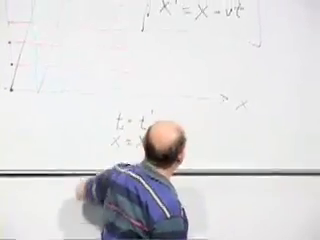
\includegraphics[width=0.72\textwidth]{lecture_01_figure_03.png}
\caption{تحويل غاليليو مكتوب بجانب شبكتي الزمكان.}
\lectureframe{00:21:57}
\end{figure}

يبين الزوج الأول للراصد المتحرك كيف يحوّل الإحداثيات التي يزوّده بها الراصد الساكن. والزوج العكسي يعيد التحويل. وهذا التحويل المتبادل بين الوصفين هو المضمون الرياضي لنسبية غاليليو.

إن الاستبدال \(t\to t'\) في الصيغة المكانية العكسية غير ضار إلا لأن نظرية غاليليو قد أعلنت بالفعل \(t=t'\). ومن المفيد أن نلحظ هذا الافتراض الآن. ففي نظرية أينشتاين سيختلف إحداثيا الزمن، ولن تعود مثل هذه الاستبدالات تلقائية.

\begin{classroomqa}
\audiencequestion{إذا حُمِلت ساعة بعيدًا ثم أُعيدت، فكيف يمكننا أن نعرف أن حركتها لم تُسرّعها أولًا ثم تُبطئها بعد ذلك، بحيث تُخفي الأثر عند مقارنة الساعات؟
\lecturetimestamp{00:23:09}}
\lecturerresponse{لم يكن في وسع غاليليو أن يثبت الزمن الكوني بدقة حديثة؛ فقد كان ذلك تخمينًا فيزيائيًا. ويمكننا اختبار هذا التخمين بطرائق كثيرة: نحمل ساعات جيدة في اتجاهين متعاكسين، ونكرر الرحلة شمالًا--جنوبًا وكذلك شرقًا--غربًا، أو نحرك ساعة حول الأخرى، أو نتبادل إشارات التوقيت من غير أن نجمع الساعات معًا. وعند السرعات العادية تتفق جميع هذه الاختبارات إلى دقة عالية جدًا. لكن مع ساعات ذات دقة كافية أو سرعات كبيرة بما فيه الكفاية يظهر بالفعل اختلاف صغير. وهذا الإخفاق للزمن الكوني ليس عيبًا في التجربة؛ بل هو إحدى الظواهر التي يجب على النسبية الخاصة أن تفسرها.}
\end{classroomqa}

\section{الثوابت الغاليليّة وقانون نيوتن}

الثابت هو كمية يتفق عليها جميع الراصدين القصوريين المعنيين هنا. وليس من الضروري أن تكون الإحداثيات نفسها ثابتة. وما يهم هو ما إذا كانت القوانين المؤلَّفة منها تحتفظ بالشكل نفسه.

تُستعمل هذه الكلمة اسمًا وصفةً معًا. فيمكن أن يكون عدد ما ثابتًا، ويمكن أن تكون معادلة ثابتةً تحت تحويل ما. والتمييز بين الكميات الثابتة والقوانين الثابتة يمنع التباسًا شائعًا: فالنسبية لا تدّعي أن كل راصد يعيّن لكل شيء الإحداثي نفسه. بل تدّعي أن القانون الفيزيائي الذي يربط قياساتهم له الشكل نفسه.

اعتبر حدثين متزامنين عند الموضعين \(x_1\) و\(x_2\). تعطي المعادلة~\eqref{eq:galilean-forward}
\begin{align}
x_1'&=x_1-vt,\\
x_2'&=x_2-vt.
\end{align}
ومن ثم فإن المسافة بينهما هي
\begin{equation}
x_2'-x_1'=(x_2-vt)-(x_1-vt)=x_2-x_1.
\end{equation}
في فيزياء غاليليو، تكون المسافة بين حدثين يقعان في الوقت نفسه ثابتة، رغم أن الموضعين المفردين ليسا كذلك.

\begin{classroomqa}
\audiencequestion{هل موضعا \(t\) في ذلك الطرح هما فعلًا الزمن نفسه؟
\lecturetimestamp{00:28:16}}
\lecturerresponse{نعم. لقد اخترنا الحدثين عمدًا ليكونا \((x_1,t)\) و\((x_2,t)\). وهما يقعان على خط أفقي واحد لزمن ثابت. ولذا فإن الحد المشترك \(vt\) يُلغى. ولو وقعت الأحداث عند أزمنة مختلفة، لما كانت هذه الحجة لتثبت فاصلًا مكانيًا لا يتغير.}
\end{classroomqa}

لنصف الآن جسيمًا بمسار \(x(t)\). ويعطي راصد القطار
\begin{equation}
x'(t)=x(t)-vt.
\end{equation}
وبأخذ المشتقة مرة واحدة نحصل على قاعدة جمع السرعات المألوفة،
\begin{equation}
\frac{dx'}{dt}=\frac{dx}{dt}-v.
\end{equation}
فالموضع والسرعة يعتمدان على الإطار المرجعي. فالراصد الذي يتحرك بمحاذاة سهم يراه يتحرك أبطأ من راصد يقف إلى جانب السكة.

خذ المشتقة مرةً أخرى. وبما أن السرعة النسبية \(v\) ثابتة،
\begin{equation}
\frac{d^2x'}{dt^2}=\frac{d^2x}{dt^2}.
\end{equation}
فالتسارع لا يتغير تحت تحويل غاليلي. وهذا يوحي بقوة بسبب كتابة قانون نيوتن بدلالة التسارع لا بدلالة الموضع أو السرعة.

هذا هو تسارع الجسم المرصود، لا تسارع راصد القطار. فكلا الإطارين عطالي، ولذلك لا يتسارع أيٌّ منهما بالنسبة إلى الآخر. وقد تتسارع الأجسام إلى اليسار أو إلى اليمين في أيٍّ من الوصفين، ويتفق الراصدان على قيمة ذلك التسارع مع أنهما يختلفان في موضع الجسم وسرعته.

افترض أن جسيمين يؤثر كلٌّ منهما في الآخر بقوة، وأن هذه القوة لا تعتمد إلا على المسافة الفاصلة بينهما عند اللحظة نفسها. هذه المسافة لا تتغير، ولذلك لا تتغير القوة. وإذا كانت الكتلة أيضًا خاصية جوهرية لا تعتمد على الإطار، فإن كل راصد عطالي يستطيع أن يكتب
\begin{equation}
F=ma
\end{equation}
بالصيغة نفسها تمامًا. فالميكانيكا النيوتنية لا تتغير تحت التحويلات الغاليلية. وليس هذا مجرد أمر معقول؛ بل هو بالغ الدقة على نحو استثنائي في مجال السرعات المألوفة كله.

تنطبق الحجة على القوى المركزية المألوفة مثل الجاذبية النيوتنية أو الكهروستاتيكا، حيث يكون المقدار دالة في المسافة. وبما أن جميع الراصدين في الأطر الغاليلية يتفقون على تلك المسافة عند زمن مشترك، فإنهم يتفقون على القوة. ومع ثبات القوة والتسارع، يقتضي الاتساق عندئذ أن يتفقوا على الكتلة أيضًا: فالجسم ذو الكيلوغرام الواحد يبقى جسمًا ذا كيلوغرام واحد عندما يمر محمولًا في قطار. وكل رمز في \(F=ma\) ينسجم مع البنية نفسها التي لا تتغير.

\section{الضوء لا ينسجم مع القاعدة الغاليلية}

الكهرومغناطيسية هي التي تولِّد هذه الصعوبة. فمعادلات ماكسويل تتنبأ بموجات تنتقل عبر الفضاء الخالي بسرعة محددة \(c\). فإذا كانت معادلات ماكسويل من قوانين الطبيعة، وكانت قوانين الطبيعة هي نفسها في كل إطار عطالي، وجب على جميع الراصدين العطاليين أن يحصلوا على القيمة نفسها \(c\).

لكن الحركيات الغاليلية تتنبأ بشيء آخر. فنبضة ضوئية تتحرك نحو اليمين في الإطار الساكن تحقق
\begin{equation}
x=ct.
\end{equation}
وبتطبيق التحويل المكاني نحصل على
\begin{equation}
x'=x-vt=(c-v)t.
\end{equation}
وبما أن \(t'=t\)، فإن راصد القطار سيقيس السرعة \(c-v\).

يمكن صياغة التناقض على نحو حاسم. فإذا احتفظت معادلات ماكسويل بصيغتها، فإنها تتنبأ بـ \(c\) في الإطار المشار إليه بشرطة. وإذا أُبقي على التحويل الغاليلي، فإنه يتنبأ بـ \(c-v\). ولا يمكن أن يكون كلاهما دقيقًا تمامًا عندما يكون \(v\ne0\).

تبدو هذه النتيجة طبيعية تمامًا إذا كان الضوء يتصرف كموجة عادية في وسط. فالقارب الذي يتحرك مع موجة مائية يقيس سرعة موجية نسبية أقل. والمستمع الذي يتحرك خلال هواء ساكن يقيس سرعةً للصوت تنزاح بسبب حركة المستمع بالنسبة إلى الهواء. ولذلك انجذب فيزيائيو القرن التاسع عشر إلى فكرة حالة سكون مفضلة، أي إطار أثيري تكون فيه معادلات ماكسويل في أبسط صورة لها ويتحرك فيه الضوء بسرعة \(c\). غير أن التجارب المصممة لكشف الحركة بالنسبة إلى مثل هذا الإطار المفضل لم تجد أثرًا مطابقًا لذلك.

كانت هناك ترتيبات تجريبية ممكنة عدة، لكن هدفها المشترك كان مقارنة انتشار الضوء لدى راصدين في حالات حركة مختلفة أو اتجاهات مختلفة للحركة. ولم يكشف أيٌّ منها عن الانزياح الغاليلي المتوقع. ولم يكن هذا الإخفاق مجرد إزعاج تقني صغير. بل فرض الاختيار بين مبدأ النسبية، ومعادلات ماكسويل، والتصورات الموروثة عن المكان والزمان.

تناول أينشتاين هذا التعارض على نحو أكثر مباشرة. فقد تخيل في شبابه أنه يطارد موجة ضوئية. ولو استطاع اللحاق بها، لتجمَّد نمطها الكهرومغناطيسي المتذبذب في الفضاء، مع أن معادلات ماكسويل لا تسمح بمثل هذه الموجة الضوئية الساكنة. فاختار أن يعدّ نظرية ماكسويل ومبدأ النسبية أمرين أساسيين، ثم يعيد النظر في الافتراضات الكامنة في إحداثياتنا.

تقوم إعادة البناء على مسلَّمتين:
\begin{enumerate}
\item تأخذ قوانين الفيزياء الصيغة نفسها في كل إطار عطالي.
\item للضوء في الفراغ السرعة نفسها \(c\) في كل إطار عطالي.
\end{enumerate}

لا يمكن للمسلَّمة الثانية أن تتعايش مع التحويل الغاليلي. فلا بد أن يتغير شيء أعمق من قاعدة جمع السرعات. وكان خيار أينشتاين الأكثر اقتصادًا هو الإبقاء على المسلَّمتين وإعادة النظر في المعادلة الغاليلية البريئة في ظاهرها \(t'=t\).

\section{مزامنة الساعات البعيدة}

يمكن تعيين المسافات المكانية بقضبان القياس، لكن الساعات البعيدة تتطلب اصطلاحًا للمزامنة. ضع ساعتين على مسافتين متساويتين من راصد في المنتصف. وعندما تقرأ كل ساعة عند الطرف الوقت المعيَّن، فلتطلق ومضة. فإذا وصلت الومضتان إلى المنتصف معًا، فاعتبر ساعتي الطرف متزامنتين. وإذا وصلت إحدى الومضتين أولًا، فاضبط الساعة المناظرة وكرر الإجراء.

وتُعرَّف كلمة \emph{المنتصف} باستخدام قضبان القياس التي سبق وضعها في ذلك الإطار. ولذلك يتضمن الاختبار عنصرين منفصلين: تساوي المسافة المكانية عن الطرفين، وتساوي زمن وصول الإشارتين. ولا يجوز إسقاط أيٍّ من هذين العنصرين. وتكرار الإجراء في أنحاء الشبكة كلها يزوِّدنا بالخطوط الأفقية ذات الزمن الثابت التي كان نيوتن قد افترضها ببساطة.

ويستخدم هذا التعريف الضوء لأن المسلَّمة تعطي الضوء السرعة نفسها في كل إطار عطالي. وما إن تُعالَج جميع الأزواج المتجاورة بهذه الطريقة حتى تحمل الشبكة كلها مجموعة متزامنة من الساعات.

ولندع الآن شبكةً ثانية تتحرك خلال الأولى. فمنتصف الجهاز المتحرك يبقى في منتصف المسافة بين طرفيه المتحركين في إطاره الخاص. أما بالنسبة إلى الجهاز الساكن، فإنه يتحرك نحو إحدى الومضتين القادمتين ويبتعد عن الأخرى. والومضتان المنبعثتان في آن واحد وفقًا للساعات الساكنة لا تصلان معًا إلى المنتصف المتحرك. وبما أن الراصد المتحرك يطبق قاعدة المنتصف والضوء نفسها، فلا يستطيع أن يعدَّ هذين الانبعاثين متزامنين. فكل إطار يزامن ساعاته الخاصة على نحو متسق، لكن عمليتي المزامنة لا تتفقان.

وهذا ليس خداعًا بصريًا ناتجًا عن محدودية زمن انتقال الضوء. فكل راصد يعلم أن الضوء يستغرق وقتًا ليصل، ويصحح أثر ذلك باستخدام السرعة نفسها \(c\). ويظل الخلاف قائمًا بعد هذا التصحيح لأن الراصدين لا يختاران الحدثين البعيدين نفسيهما على أنهما زوج متزامن. فالتزامن نفسه، لا مجرد مظهر التزامن، نسبي.

\begin{classroomqa}
\audiencequestion{هل يمكننا تجنب هذا الاستنتاج بمزامنة الساعات بالصوت بدلًا من الضوء؟
\lecturetimestamp{00:49:03}}
\lecturerresponse{يصلح الصوت إشارةً للمزامنة في إطار يكون فيه الهواء ساكنًا، لكن سرعته المقاسة ليست هي نفسها في كل إطار عطالي. فالقطار المفتوح الذي يتحرك خلال هواء ساكن يكون متحركًا بالنسبة إلى الوسط الحامل للصوت، ولذلك لا تتصرف إشارات الصوت المتجهة إلى الأمام وإلى الخلف فيه على نحو متناظر. أما الضوء فمختلف بحسب المسلَّمة: لا يوجد وسط بصري قابل للكشف يحدد إطار سكونه راصدًا بعينه. ولذلك نستخدم الضوء ونتبع النتائج المترتبة على ذلك.}
\end{classroomqa}

أصبح الخلاف النوعي واضحًا. ونحسب الآن على وجه الدقة أيَّ الأحداث يعدها الراصد المتحرك متزامنة.

\section{بناء أشعة الضوء}

ولأجل هذا البناء، من الملائم اختيار وحدات بحيث
\begin{equation}
c=1.
\end{equation}
وعندئذ تكون وحدة المسافة هي المسافة التي يقطعها الضوء في وحدة واحدة من الزمن: ثوانٍ ضوئية مقترنة بثوانٍ، أو سنوات ضوئية مقترنة بسنوات. ويُقاس المكان والزمان بالوحدات نفسها، وتكون السرعات بلا أبعاد، وتظهر أشعة الضوء عند \(45^\circ\). فالشعاع المتحرك نحو اليمين يحقق
\begin{equation}
x=t+d,
\end{equation}
بينما يحقق الشعاع المتحرك نحو اليسار
\begin{equation}
x=-t+d'.
\end{equation}
وأما الشعاعان الماران بنقطة الأصل فهما ببساطة \(x=t\) و\(x=-t\). وتقع المسارات الزمنية، التي تخص أجسامًا أبطأ من الضوء، أقرب إلى المحور الرأسي. أما مسار افتراضي أسرع من الضوء فسيقع أقرب إلى المحور الأفقي.

لا تصبح الزاوية في الرسم ذات معنى إلا بعد اختيار هذه الوحدات. فبوحدتي المتر والثانية سيبدو الشعاع الضوئي أفقيًا تقريبًا لأنه يقطع نحو \(3\times10^8\) متر في ثانية واحدة. واختيار الثواني الضوئية للمسافة يعيد تحجيم المحور الأفقي ويجعل الهندسة السببية مرئية.

اعتبر ثلاثة خطوط عالم متوازية في الشبكة المتحركة،
\begin{equation}
x=vt,\qquad x=vt+L,\qquad x=vt+2L.
\label{eq:moving-worldlines}
\end{equation}
ينتمي خط العالم الأوسط إلى الراصد الذي يختبر التزامن بين النقطتين الطرفيتين. تتحرك النقاط الثلاث بانتظام وتحافظ على ترتيبها النسبي في الإطار ذي الشرطة.

\begin{figure}[H]
\centering
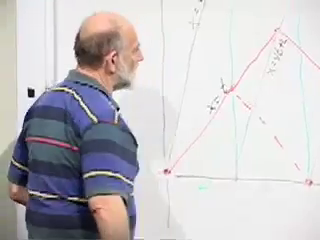
\includegraphics[width=0.72\textwidth]{lecture_01_figure_04.png}
\caption{الشعاع الضوئي المتجه إلى الأمام \(x=t\) عند التقائه بخط العالم المتحرك الأوسط.}
\lectureframe{01:02:33}
\end{figure}

يمكن رسم الهندسة الكاملة من دون أن يحجبها شخص واقف أمام اللوح:

\begin{figure}[H]
\centering
\begin{tikzpicture}[scale=0.95]
\draw[->] (-0.5,0) -- (6.5,0) node[right] {$x$};
\draw[->] (0,-0.2) -- (0,4.3) node[above] {$t$};
\draw[blue] (0,0) -- (1.4,4.0);
\draw[blue] (2.0,0) -- (3.4,4.0);
\draw[blue] (4.0,0) -- (5.4,4.0);
\draw[red] (0,0) -- (3.08,3.08);
\draw[red] (3.08,3.08) -- (4.56,1.60);
\draw[red,dashed] (2.0,0) -- (4.56,1.60);
\fill (0,0) circle (1.5pt);
\fill (2.0,0) circle (1.5pt);
\fill (4.0,0) circle (1.5pt);
\fill (3.08,3.08) circle (1.5pt);
\fill (4.56,1.60) circle (1.5pt);
\node[left] at (0.55,1.55) {$x=vt$};
\node[left] at (2.45,1.9) {$x=vt+L$};
\node[right] at (4.72,1.9) {$x=vt+2L$};
\node[left] at (1.88,2.28) {$x=t$};
\node[above right] at (3.08,3.08) {$A$};
\end{tikzpicture}
\caption{تحدد الإشارات الضوئية خط التزامن في الإطار المتحرك.}
\end{figure}

أرسل شعاعًا ضوئيًا متجهًا إلى اليمين من الأصل. لتكن \(A\) نقطة تقاطعه مع خط العالم الأوسط. والمعادلتان عند \(A\) هما
\begin{align}
x&=t,\\
x&=vt+L.
\end{align}
وبالتعويض نحصل على
\begin{equation}
t=vt+L,
\end{equation}
ومن ثم
\begin{equation}
t_A=x_A=\frac{L}{1-v}.
\label{eq:point-a}
\end{equation}

ابتداءً من \(A\)، تتبَّع شعاعًا ضوئيًا متجهًا إلى اليسار رجوعًا حتى خط العالم المتحرك الأيمن. معادلته تأخذ الصورة
\begin{equation}
x+t=b.
\end{equation}
ولأنه يمر عبر \(A\)، فإن المعادلة~\eqref{eq:point-a} تحدد الثابت:
\begin{equation}
b=x_A+t_A=\frac{2L}{1-v}.
\end{equation}
ولذلك يحقق الشعاع الراجع
\begin{equation}
x+t=\frac{2L}{1-v}.
\label{eq:backward-ray}
\end{equation}

ويُستنتَج تقاطعه مع خط العالم الأيمن من
\begin{align}
x+t&=\frac{2L}{1-v},\\
x&=vt+2L.
\end{align}
وبحذف \(x\)،
\begin{align}
(1+v)t
  &=2L\left(\frac{1}{1-v}-1\right)\\
  &=\frac{2Lv}{1-v},
\end{align}
إذن
\begin{equation}
t=\frac{2Lv}{1-v^2}.
\end{equation}
وبالتعويض في \(x=vt+2L\) نحصل على
\begin{equation}
x=\frac{2L}{1-v^2}.
\end{equation}
الإحداثيات نفسها أقل أهمية من نسبتها:
\begin{equation}
\frac{t}{x}=v.
\end{equation}
ومن ثم فإن كل حدث متزامن مع الأصل وفقًا للساعات المتحركة يقع على
\begin{equation}
t=vx,
\label{eq:simultaneity-c-one}
\end{equation}
بينما يتبع أصل الإطار المتحرك
\begin{equation}
x=vt.
\label{eq:moving-time-axis}
\end{equation}
والمحوران مائلان تناظريًا حول شعاع الضوء عند \(45^\circ\).

كل النقاط على \(x=vt\) لها الموضع ذو الشرطة نفسه، \(x'=0\)، بينما تختلف أزمنتها ذات الشرطة. وكل النقاط على \(t=vx\) لها الزمن ذو الشرطة نفسه، \(t'=0\)، بينما تختلف مواضعها ذات الشرطة. ولذلك فإن الأول هو محور الزمن ذي الشرطة والآخر محور المكان ذي الشرطة. وكان بناء الإشارات الطويل ضروريًا لتعيين الخط الثاني؛ إذ لم يكن من الممكن استنتاجه من خط العالم المتحرك وحده.

إن إرجاع الوحدات المعتادة في المعادلة~\eqref{eq:simultaneity-c-one} يتطلب
\begin{equation}
t=\frac{v}{c^2}x.
\label{eq:simultaneity-dimensional}
\end{equation}
ويفسر العامل \(c^2\) لماذا تعمل الصورة النيوتنية جيدًا إلى هذا الحد في الحياة اليومية. فعند السرعات الصغيرة جدًا مقارنةً بـ \(c\)، يكون ميل خط التزامن المتحرك صغيرًا للغاية.

\begin{figure}[H]
\centering
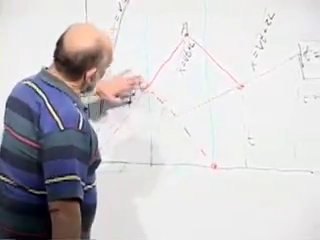
\includegraphics[width=0.72\textwidth]{lecture_01_figure_05.png}
\caption{مع \(c=1\)، يكون محورا الزمن ذي الشرطة والتزامن متماثلين حول شعاع الضوء.}
\lectureframe{01:15:40}
\end{figure}

\begin{figure}[H]
\centering
\begin{tikzpicture}[scale=1.0]
\draw[->] (-2.2,0) -- (5.2,0) node[right] {$x$};
\draw[->] (0,-0.2) -- (0,4.9) node[above] {$t$};
\draw[red] (0,0) -- (3.9,3.9);
\draw[red] (0,0) -- (-1.8,1.8);
\draw[blue] (0,0) -- (1.8,4.5);
\draw[blue,dashed] (0,0) -- (4.5,1.8);
\node[right] at (3.9,3.9) {$x=t$};
\node[left] at (-1.8,1.8) {$x=-t$};
\node[above] at (1.8,4.5) {$x'=0$};
\node[right] at (4.5,1.8) {$t'=0$};
\end{tikzpicture}
\caption{المحاور ذات الشرطة وأشعة الضوء الثابتة في وحدات \(c=1\).}
\end{figure}

\section{اشتقاق تحويل لورنتز}

تحدد الهندسة المواضع التي تنعدم عندها كل إحداثية ذات شرطة. فعلى امتداد محور الزمن المتحرك \(x=vt\)، يجب أن يكون \(x'=0\). وعلى امتداد محور التزامن المتحرك \(t=vx\)، يجب أن يكون \(t'=0\). ويمكن كتابة أعم العلاقات الخطية الموافقة لمواضع الانعدام هذه على الصورة
\begin{align}
x'&=\frac{x-vt}{F(v)},\\
t'&=\frac{t-vx}{G(v)}.
\label{eq:fg-ansatz}
\end{align}
ويسمح العاملان \(F\) و\(G\) بأن تختلف مقاييس الإحداثيات ذات الشرطة عن المقاييس الغاليلية، مع أن موضعي المحورين قد تحددا بالفعل. وتنتج الخطية من تجانس المكان والزمان: فنقل تجربة من موضع إلى آخر لا يمكن أن يغيّر قانون التحويل.\editorialnote{هذه الحجة الموجزة للخطية تُصرِّح بافتراض استُخدم ضمنًا في الاشتقاق على اللوح.}

في هذه المرحلة أخبرتنا الهندسة بالكثير، ولكن ليس بكل شيء. فالبسطان يحددان ميل المحورين، لكنهما لا يحددان تباعد الوحدات على امتدادهما. وهذه المعلومة المقياسية المتبقية هي بالضبط ما يمثله \(F(v)\) و\(G(v)\).

لنفرض الآن ثبات سرعة الضوء. فشعاع متجه إلى اليمين يحقق \(x=t\) يجب أن يحقق أيضًا \(x'=t'\). وعلى طول ذلك الشعاع،
\begin{align}
x'&=\frac{(1-v)t}{F(v)},\\
t'&=\frac{(1-v)t}{G(v)}.
\end{align}
ولكي تتحقق المساواة عند كل نقطة على الشعاع، لا بد من أن
\begin{equation}
F(v)=G(v).
\end{equation}
ولذلك يمكننا أن نكتب
\begin{align}
x'&=\frac{x-vt}{F(v)},\\
t'&=\frac{t-vx}{F(v)}.
\label{eq:common-f}
\end{align}

تستخدم هذه الخطوة أول مطلب أينشتايني حقيقي في الجبر. فالخط الهندسي نفسه هو شعاع ضوئي بالنسبة إلى كلا الراصدين، لذا يجب أن يزداد الإحداثيان ذوا الشرطة بالمقدار نفسه على امتداده عندما يكون \(c=1\). ولو اختلف العاملان في المعادلتين لكانت السرعة ذات الشرطة مختلفة عن الواحد.

يبقى تابع مجهول واحد. اضرب المعادلة~\eqref{eq:common-f} في \(F(v)\):
\begin{align}
F(v)x'&=x-vt,\\
F(v)t'&=t-vx.
\end{align}
وبضرب المعادلة الثانية في \(v\) ثم جمعها مع الأولى يُحذَف \(t\)، فنحصل على
\begin{equation}
(1-v^2)x=F(v)(x'+vt').
\end{equation}
وبالمثل،
\begin{equation}
(1-v^2)t=F(v)(t'+vx').
\end{equation}
ولذلك يكون التحويل العكسي
\begin{align}
x&=\frac{F(v)}{1-v^2}(x'+vt'),\\
t&=\frac{F(v)}{1-v^2}(t'+vx').
\end{align}

يجعل مبدأ النسبية العلاقة بين الإطارين تبادلية. فإذا رأت المحطة القطار يتحرك بسرعة \(+v\)، فإن القطار يرى المحطة تتحرك بسرعة \(-v\). وبناءً على ذلك، يجب أن تكون المعادلات العكسية على الصورة نفسها التي للمعادلات الأمامية مع عكس إشارة \(v\). ويجب أن تحقق معاملاتها الأمامية
\begin{equation}
\frac{F(v)}{1-v^2}=\frac{1}{F(v)}.
\end{equation}
ومن ثم
\begin{equation}
F(v)^2=1-v^2,
\end{equation}
ويختار الاتصال مع تحويل الهوية عند \(v=0\) الجذر الموجب،
\begin{equation}
F(v)=\sqrt{1-v^2}.
\end{equation}

لم تُواءَم النتيجة مع نبضة ضوئية بعينها. فهي تنشأ من المحاور التي يثبتها التزامن، ومن السرعة المشتركة للضوء، ومن اشتراط ألا يُمنَح أي إطار قصوري امتيازًا على الآخر.

تحويل لورنتز بوحدات يكون فيها \(c=1\) هو
\begin{align}
x'&=\frac{x-vt}{\sqrt{1-v^2}},\\
t'&=\frac{t-vx}{\sqrt{1-v^2}}.
\label{eq:lorentz-c-one}
\end{align}
ومعكوسه هو
\begin{align}
x&=\frac{x'+vt'}{\sqrt{1-v^2}},\\
t&=\frac{t'+vx'}{\sqrt{1-v^2}}.
\end{align}

\begin{figure}[H]
\centering
\includegraphics[width=0.76\textwidth]{lecture_01_figure_06.png}
\caption{تحويل لورنتز المكتمل في وحدات \(c=1\) على اللوح.}
\lectureframe{01:32:38}
\end{figure}

تظهر الحداثة الأساسية بالفعل في معادلة الزمن. فالزمن لا يُنقل ببساطة من إطار إلى آخر من دون تغيّر. إذ يمزج إحداثي الزمن ذي الشرطة بين الزمن والموضع في الإطار غير المعلَّم بالشرطة. ونتيجةً لذلك، فإن \(t=\text{constant}\) و\(t'=\text{constant}\) يصفان مجموعتين مختلفتين من الأحداث.

حدّ المزج ليس تصحيحًا اختياريًا يُلحَق لاحقًا. فبدونه سيبقى الخط \(t'=0\) أفقيًا، وسيظل تزامن الأحداث البعيدة كونيًا، ولن يستطيع التحويل أن يحفظ سرعة الضوء.

\section{استعادة سرعة الضوء والتحقق من النتيجة}

عندما يكون \(c\ne1\)، يعيد الاتساق البعدي العوامل الناقصة. فالنسبة \(v^2/c^2\) لا بُعدية، بينما \((v/c^2)x\) له وحدات زمن. ومن ثم
\begin{align}
x'&=\frac{x-vt}{\sqrt{1-v^2/c^2}},\\
t'&=\frac{t-(v/c^2)x}{\sqrt{1-v^2/c^2}}.
\label{eq:lorentz-dimensional}
\end{align}
ويُحصَل على المعكوس بعكس إشارة \(v\):
\begin{align}
x&=\frac{x'+vt'}{\sqrt{1-v^2/c^2}},\\
t&=\frac{t'+(v/c^2)x'}{\sqrt{1-v^2/c^2}}.
\end{align}
ومن شأن إدخال
\begin{equation}
\gamma=\frac{1}{\sqrt{1-v^2/c^2}}
\end{equation}
أن يضع هذه المعادلات في الصيغة الموجزة المألوفة، لكن صيغة المقام تُبقي الاشتقاق ظاهرًا.

عدديًا، \(c\simeq3\times10^8\,\mathrm{m/s}\)، ومن ثم \(c^2\simeq9\times10^{16}\,\mathrm{m^2/s^2}\). ويجعل هذا المقام الكبير كلاً من ميل خط التزامن والعامل \(v^2/c^2\) غير ملحوظين في معظم التجارب الميكانيكية. وهذا الصغر يفسر نجاح غاليليو؛ لكنه لا يعيد الزمن المطلق.

\begin{figure}[H]
\centering
\includegraphics[width=0.76\textwidth]{lecture_01_figure_07.png}
\caption{تحويل لورنتز بعد استعادة عوامل \(c\).}
\lectureframe{01:35:58}
\end{figure}

هناك اختباران مباشران. خذ أولًا \(v\ll c\). عندئذٍ يكون \(v^2/c^2\) مهمَلًا، وللمسافات العادية يكون حد نسبية التزامن \(vx/c^2\) مهمَلًا أيضًا. وتختزل المعادلة~\eqref{eq:lorentz-dimensional} إلى
\begin{equation}
t'\approx t,\qquad x'\approx x-vt.
\end{equation}
وتُستعاد النسبية الغاليلية بوصفها تقريب السرعات المنخفضة.

ثانيًا، اختبر شعاعًا ضوئيًا. فبعد استعادة \(c\)، يحقق الشعاع المتجه إلى اليمين \(x=ct\)، لا \(x=t\). ويعطي التعويض
\begin{align}
x'&=\frac{(c-v)t}{\sqrt{1-v^2/c^2}},\\
t'&=\frac{(1-v/c)t}{\sqrt{1-v^2/c^2}}.
\end{align}
وبما أن \(c-v=c(1-v/c)\)،
\begin{equation}
x'=ct'.
\end{equation}
فإن الراصد في الإطار ذي الشرطة يقيس السرعة نفسها \(c\). وبالنسبة إلى شعاع متجه إلى اليسار، فإن التعويض عن \(x=-ct\) يعطي بالمثل
\begin{equation}
x'=-ct'.
\end{equation}
ويتعامل التحويل مع الضوء المتحرك في أي من الاتجاهين على نحو صحيح.

إن التمييز بين \(x=t\) و\(x=ct\) فحصٌ بُعديٌّ مفيد. فالأولى صحيحة فقط في وحدات يكون فيها \(c=1\). وإن استعادة الوحدات المعتادة في التحويل مع إبقاء معادلة الشعاع في الوحدات الطبيعية سيخلط بين اصطلاحين ويؤدي إلى نتيجة خاطئة. ويلتقط الاتساق البعدي هذا الخطأ فورًا.

\section{معيار نقطة المنتصف}

\begin{classroomqa}
\audiencequestion{افترض أن راصدًا يستقبل وميضين في اللحظة نفسها، لكنه ليس في منتصف المسافة بين مصدريهما. فهل يجوز لذلك الراصد أن يستنتج أن الوميضين قد انبعثا في آن واحد؟
\lecturetimestamp{01:42:55}}
\lecturerresponse{لا. إن تساوي زمنَي الوصول لا يستلزم تساوي زمنَي الانبعاث إلا بالنسبة إلى الراصد الواقع مكانيًا في منتصف المسافة بين المصدرين في الإطار المعني. فالمستقبِل الأقرب إلى أحد المصدرين قد يتلقى الوميضين معًا مع أن الوميض الأبعد قد انبعث أبكر. ولذلك فإن خط عالم المنتصف \(x=vt+L\) أساسي في البنية المتحركة. ويُتتبَّع الشعاع المتجه إلى الأمام \(x=t\) حتى يلتقي بخط المنتصف ذاك، ثم يُتتبَّع شعاع ضوئي راجع حتى \(x=vt+2L\). وذلك الحدث الطرفي الثاني، لا حدث وصول متساوٍ اعتباطي في موضع آخر، هو المتزامن مع الأصل وفقًا للإطار المتحرك.}
\end{classroomqa}

لقد بلغنا تحويل الإحداثيات الكامل، ولكننا لم نصل بعد إلى أشهر نتائجه. ويأتي بعد ذلك تقلص الطول وتمدد الزمن والزمن الخاص، ثم الزخم والطاقة النسبيان. والأساس قائم بالفعل: فلا يستطيع كل إطار قصوري أن يستخدم القوانين نفسها ويقيس سرعة الضوء نفسها إلا لأن المكان والزمان يمتزجان، ولأن تزامن الأحداث البعيدة ينتمي إلى إطار ما بدلًا من أن ينتمي إلى العالم على نحو مطلق.
\chapter{معادلات ماكسويل، والتغاير، والموجات الكهرومغناطيسية}

\lectureoverview{تؤثر المجالات الكهربائية والمغناطيسية في المادة المشحونة عبر قوة لورنتز، لكن لا بد أيضًا أن تُنشئ المادة هذه المجالات وأن تعيد ترتيبها. سنصوغ ذلك النصف المتبادل من الكهرومغناطيسية، ونبيّن أن معادلات ماكسويل متغايرة لورنتزيًا، ونشتق حلولها الموجية، ثم نعيد إدخال الشحنة والتيار بصيغة تجعل الانحفاظ الموضعي ظاهرًا بجلاء. وطوال هذه المحاضرة نستخدم وحدات يكون فيها \(c=1\).}

\section{النصف الآخر من الكهرومغناطيسية}

لنبدأ بالجزء الذي صار بين أيدينا من الموضوع. إذا تحرك جسيم شحنته \(q\) بسرعة \(\mathbf v\) عبر مجالين كهربائي ومغناطيسي، فإن القوة هي
\begin{equation}
\mathbf F=q\bigl(\mathbf E+\mathbf v\times\mathbf B\bigr).
\label{eq:lorentz-force-three}
\end{equation}
إن العامل \(q\) لا غنى عنه. فالجسيم غير المشحون لا يتأثر بالقوة الكهرومغناطيسية. ويسهم المجال الكهربائي حتى عندما يكون الجسيم ساكنًا آنيًا، في حين تعتمد المساهمة المغناطيسية على حركته.

تخبرنا المعادلة~\eqref{eq:lorentz-force-three} بما تفعله المجالات المعطاة بالمادة. لكنها لا تخبرنا بما يحدد المجالات نفسها. ما الذي يولد مجالًا كهربائيًا حول جسم، ومجالًا مغناطيسيًا حول آخر، أو موجةً تتحرك عبر الفضاء الخالي؟ المعادلات التي تجيب عن هذه الأسئلة هي معادلات ماكسويل.

\begin{figure}[H]
\centering
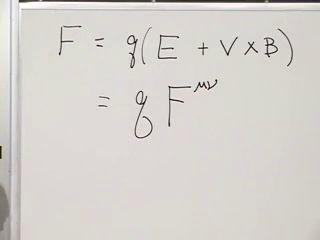
\includegraphics[width=0.62\textwidth]{lecture_58_figure_02.png}
\caption{قوة لورنتز بصيغة المتجه الثلاثي وبداية إعادة صياغتها الموترية.}
\lectureframe{00:05:49}
\end{figure}

تستبق الصيغة النسبية لقانون القوة الترميز الذي سنحتاج إليه:
\begin{equation}
f^\mu=qF^\mu{}_{\nu}u^\nu.
\label{eq:lorentz-force-four}
\end{equation}
هنا \(u^\nu\) هو السرعة الرباعية، و\(f^\mu\) هو القوة الرباعية، و\(F^{\mu\nu}\) موتر مضاد للتماثل مُركَّب من \(\mathbf E\) و\(\mathbf B\). ويعرض اللوح أولًا مجرد بداية تخطيطية لهذا التعبير؛ ويزوّدنا الانكماش مع \(u^\nu\) بالمتجه المفقود اللازم لترك فهرس قوة واحد حرًا.

هناك سبب فيزيائي يقتضي أن تؤثر المادة بدورها في المجال. فبإمكان موجة كهرومغناطيسية أن تصطدم بشحنة، فتسرّعها وتنقل إليها طاقة. ولو كان المجال يستطيع التأثير في الشحنة بينما لا تستطيع الشحنة قط التأثير في المجال، لما وُجد موضع سُحبت منه تلك الطاقة. وليس الفعل ورد الفعل تمام الحجة كلها، لكن انحفاظ الطاقة يجعل الاقتران المتبادل أمرًا لا مفر منه.

\section{مصدر متغير يبعث اضطرابًا}

تنتج الشحنة النقطية مجالًا كهربائيًا يتجه إلى الخارج من موضعها أو إلى داخله. وينتج تيار في سلك--أي تدفق جسيمات مشحونة--مجالًا مغناطيسيًا يدور حول السلك. وهذه الصور الساكنة المألوفة تُظهر بالفعل نمطين هندسيين مختلفين: فالفيض الكهربائي ينبعث من الشحنة، بينما تلتف خطوط المجال المغناطيسي حول التيار.

والآن حرّك الشحنة النقطية فجأة. بالقرب من موضعها الجديد لا بد أن يبدأ المجال الكهربائي بإعادة ترتيب نفسه، لكن مراقبًا بعيدًا لا يستطيع أن يعلم بالحركة على الفور. ويبقى المجال القديم بعيدًا إلى أن تتاح لإشارة فرصة الوصول. وبين المنطقتين القريبة والبعيدة تقع جبهة متحركة يتغير عندها المجال. وهذه إعادة الترتيب المتحركة هي اضطراب كهرومغناطيسي.

إذا أُجبرت الشحنة على الحركة ذهابًا وإيابًا، فإن عمليات إعادة ترتيب متعاقبة تتلو بعضها بعضًا وتشكّل موجة كهرومغناطيسية. وهذه هي الوظيفة الأولية للهوائي: تيار كهربائي متذبذب يبعث اضطرابًا في المجال إلى الخارج. ويعطي عكس تيار في سلك النسخة المغناطيسية من الحجة نفسها. فلا بد أن ينعكس دوران \(\mathbf B\)، لكن هذا الانعكاس ينتشر بدلًا من أن يظهر في كل مكان دفعة واحدة.

تضع هذه الصورة السببية هدفين لمعادلات ماكسويل. فلا بد أن تصف كيف تكون الشحنة والتيار مصدرين للمجالات، ولا بد أن تسمح بأن تنتشر التغيرات في تلك المجالات بسرعة لا تتجاوز سرعة الضوء. والهدف الثاني هو أيضًا اختبار للنسبية. فإذا كانت معادلات ماكسويل تأخذ الصيغة نفسها في كل إطار قصوري وتستلزم سرعة موجية محددة، فلا بد أن يستنتج كل إطار قصوري السرعة نفسها منها.

\section{مراجعة معادلة الموجة النسبية}

قبل الانتقال إلى المجالات المتجهية، تأمل مجالًا قياسيًا \(\phi(\mathbf x,t)\)، أي عددًا واحدًا عند كل نقطة من الزمكان. إن معادلة من الرتبة الأولى
\begin{equation}
\partial_\mu\phi=0
\end{equation}
كانت لتقول إن كل مشتقة زمكانية تنعدم. وعندئذ يكون المجال ثابتًا، ومن ثم غير قادر على حمل موجة. أما معادلة موجة نسبية غير تافهة فتستخدم مشتقتين:
\begin{equation}
\partial_\mu\partial^\mu\phi=0.
\end{equation}
ومع اصطلاح الإشارة المستخدم هنا،
\begin{equation}
\left(\partial_t^2-\partial_x^2-\partial_y^2-\partial_z^2\right)\phi=0,
\label{eq:scalar-wave-four}
\end{equation}
أو، بصورة أكثر اختصارًا،
\begin{equation}
\left(\partial_t^2-\nabla^2\right)\phi=0.
\end{equation}
ويجعل الاختيار \(c=1\) الزمن والمسافة يحملان وحدات متوافقة. وإذا أعدنا الوحدات المعتادة فسيظهر \(1/c^2\) إلى جانب المشتقة الزمنية الثانية.

بالنسبة إلى موجة تسير على طول المحور \(z\)، يعتمد المجال على \(z\) و\(t\)، لا على \(x\) أو \(y\). وتُختزل المعادلة~\eqref{eq:scalar-wave-four} إلى
\begin{equation}
\left(\partial_t^2-\partial_z^2\right)\phi=0.
\label{eq:scalar-wave-one}
\end{equation}

\begin{figure}[H]
\centering
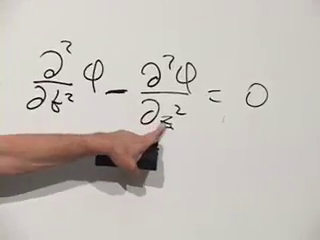
\includegraphics[width=0.56\textwidth]{lecture_58_figure_04.png}
\caption{معادلة الموجة القياسية أحادية البعد المستخدمة نموذجًا للموجات الكهرومغناطيسية.}
\lectureframe{00:47:03}
\end{figure}

وصيغتها العامة لموجة منتقلة هي
\begin{equation}
\phi(z,t)=f(z-t)+g(z+t).
\end{equation}
تتحرك الهيئة \(f(z-t)\) نحو تزايد \(z\)، لأن نقطة ذات طور ثابت تحقق \(z-t=\text{constant}\). أما الهيئة \(g(z+t)\) فتتحرك في الاتجاه المعاكس. ولا شيء يفرض أن تكون أي من الهيئتين جيبية؛ فأي شكل أملس بما يكفي ينتقل من غير أن يغيّر شكله.

ومع ذلك تبقى الدوال الجيبية ملائمة:
\begin{equation}
\phi(z,t)=A\cos\!\bigl(k(z-t)\bigr).
\end{equation}
ويتحكم عدد الموجة \(k\) في الطول الموجي،
\begin{equation}
\lambda=\frac{2\pi}{k}.
\end{equation}
فالقيمة الكبيرة لـ\(k\) تولّد تذبذبًا مكانيًا سريعًا وطولًا موجيًا قصيرًا؛ أما القيمة الصغيرة لـ\(k\) فتولّد طولًا موجيًا طويلًا. وهذه الهيئات نفسها ستصبح بعد قليل مركبات \(\mathbf E\) و\(\mathbf B\).

\section{حساب المتجهات الذي تحتاج إليه معادلات ماكسويل}

تُكتب معادلات ماكسويل باستخدام الجداء النقطي، والجداء الاتجاهي، والتباعد، والدوران. ويستحق الأمر أن نعيد بناء هذا الترميز مرة واحدة، لأن حسابات المركبات اللاحقة تستخدم هذه الأنماط نفسها على وجه الدقة.

بالنسبة إلى المتجهين الثلاثيين العاديين \(\mathbf a\) و\(\mathbf b\)، فالجداء النقطي هو الكمية القياسية
\begin{equation}
\mathbf a\cdot\mathbf b
=a_xb_x+a_yb_y+a_zb_z.
\end{equation}
أما الجداء الاتجاهي فهو متجه آخر،
\begin{align}
(\mathbf a\times\mathbf b)_x&=a_yb_z-a_zb_y,\\
(\mathbf a\times\mathbf b)_y&=a_zb_x-a_xb_z,\\
(\mathbf a\times\mathbf b)_z&=a_xb_y-a_yb_x.
\end{align}
وتتبع المركبات الباقية من الترتيب الدوري \(x\to y\to z\to x\).

لنعرّف المؤثر التفاضلي
\begin{equation}
\boldsymbol\nabla=
\left(\partial_x,\partial_y,\partial_z\right).
\end{equation}
فمدخلاته مؤثرات لا أعداد عادية، لكن لا يزال بالإمكان استخدام نمطي الجداء النقطي والاتجاهي. وبالنسبة إلى مجال متجهي \(\mathbf A\)، فإن
\begin{equation}
\boldsymbol\nabla\cdot\mathbf A
=\partial_xA_x+\partial_yA_y+\partial_zA_z
\label{eq:divergence}
\end{equation}
هو التباعد، بينما
\begin{align}
(\boldsymbol\nabla\times\mathbf A)_x
 &=\partial_yA_z-\partial_zA_y,\\
(\boldsymbol\nabla\times\mathbf A)_y
 &=\partial_zA_x-\partial_xA_z,\\
(\boldsymbol\nabla\times\mathbf A)_z
 &=\partial_xA_y-\partial_yA_x
\label{eq:curl}
\end{align}
هي مركبات الدوران.

الهندسة لا تقل أهمية عن الصيغ. يكون للمجال المتجهي تباعد موجب حيث يبدو أنه يتدفق إلى الخارج من مصدر. ويكون له دوران حيث يدور. ويجسّد المجال الكهربائي الشعاعي لشحنة نقطية التباعد؛ ويجسّد المجال المغناطيسي الملتف حول سلك يحمل تيارًا الدوران. أما المجال المتجهي الثابت مكانيًا فلا يملك أيًا منهما.

\section{معادلات ماكسويل في الفراغ}

في غياب الشحنة والتيار، تكون معادلات ماكسويل هي
\begin{align}
\boldsymbol\nabla\times\mathbf E&=-\partial_t\mathbf B,
\label{eq:faraday-vac}\\
\boldsymbol\nabla\cdot\mathbf B&=0,
\label{eq:gauss-b-vac}\\
\boldsymbol\nabla\times\mathbf B&=\partial_t\mathbf E,
\label{eq:ampere-vac}\\
\boldsymbol\nabla\cdot\mathbf E&=0.
\label{eq:gauss-e-vac}
\end{align}
تكاد معادلتا الدوران أن تتبادلا \(\mathbf E\) و\(\mathbf B\)، لكن إشارة سالب أساسية تميّزهما. وتقول معادلتا التباعد إن أيًا من المجالين لا يملك مصدرًا في منطقة الفراغ موضع النظر. ويظل تباعد المجال المغناطيسي صفرًا حتى بعد إعادة المصادر الكهربائية؛ فالكهرومغناطيسية العادية لا تتضمن شحنة مغناطيسية.

\begin{figure}[H]
\centering
\includegraphics[width=0.76\textwidth]{lecture_58_figure_06.png}
\caption{معادلات ماكسويل الأربع في الفراغ، مرتبة لإظهار التناظر القريب بين المجالين الكهربائي والمغناطيسي.}
\lectureframe{00:27:30}
\end{figure}

ستحل كثافة الشحنة \(\rho\) في النهاية محل الصفر على الطرف الأيمن من المعادلة~\eqref{eq:gauss-e-vac}، وستدخل كثافة التيار \(\mathbf J\) في المعادلة~\eqref{eq:ampere-vac}. ونؤجل هذين الحدين مؤقتًا. فالمعادلات الخالية من المصدر تكشف بنية التحول وآلية الموجة بأقل قدر من التشويش.

كما أنها تزيد أحجية أينشتاين حدّة. فالمراقب الغاليلي الذي يتبع موجة سيتوقع أن يطرح السرعات وأن يقيس سرعة موجية أصغر. ومع ذلك، إذا كانت معادلات ماكسويل نفسها تصح في كل إطار قصوري، فإن كل مراقب يستنبط منها السرعة الموجية الوحدوية نفسها. وليس المخرج هو تغيير معادلة الموجة من إطار إلى إطار، بل استخدام تحويل لورنتز وإظهار معادلات ماكسويل على هيئة كميات صارت قوانين تحولها معروفة سلفًا.

\section{المجالان الكهربائي والمغناطيسي بوصفهما موترًا واحدًا}

يتحد المجالان الكهربائي والمغناطيسي في موتر المجال المضاد للتماثل
\begin{equation}
F^{\mu\nu}=
\begin{pmatrix}
0   & -E_x & -E_y & -E_z\\
E_x & 0    & -B_z & B_y\\
E_y & B_z  & 0    & -B_x\\
E_z & -B_y & B_x  & 0
\end{pmatrix},
\label{eq:l0203-field-tensor}
\end{equation}
حيث ترتيب الصفوف والأعمدة هو \(t,x,y,z\). ويفرض التضاد في التماثل،
\begin{equation}
F^{\mu\nu}=-F^{\nu\mu},
\end{equation}
أن تنعدم العناصر القطرية وأن يُحدَّد النصف السفلي من المصفوفة من نصفها العلوي. وتحتوي العناصر المختلطة زمانًا ومكانًا على \(\mathbf E\)؛ أما العناصر المكانية الخالصة فتحتوي على \(\mathbf B\).

\begin{figure}[H]
\centering
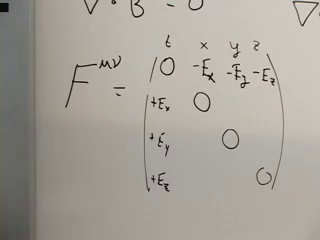
\includegraphics[width=0.58\textwidth]{lecture_58_figure_03.png}
\caption{موتر المجال الكهرومغناطيسي المكتمل، بما في ذلك عناصره الكهربائية والمغناطيسية.}
\lectureframe{00:32:05}
\end{figure}

ليست أهمية \(F^{\mu\nu}\) مجرد أن مركبات المجال الست تنتظم في مصفوفة واحدة. فعند تحويل لورنتز يتحول كموتر من الرتبة الثانية. ولذلك يختلط المجالان الكهربائي والمغناطيسي كما يقيسهما مراقبون مختلفون على النحو المطلوب تمامًا لكي يتحول الكل تحوّلًا متسقًا.

يوجد موترٌ مضادّ التناظر ثانٍ، هو موتر المجال المزدوج \(\widetilde F^{\mu\nu}\). ووفق الاصطلاح المعتمد هنا يُحصَل عليه من المعادلة~\eqref{eq:l0203-field-tensor} بالاستبدال
\begin{equation}
\mathbf E\longmapsto-\mathbf B,
\qquad
\mathbf B\longmapsto\mathbf E.
\label{eq:dual-replacement}
\end{equation}
ومن ثم
\begin{equation}
\widetilde F^{\mu\nu}=
\begin{pmatrix}
0    & B_x  & B_y  & B_z\\
-B_x & 0    & -E_z & E_y\\
-B_y & E_z  & 0    & -E_x\\
-B_z & -E_y & E_x  & 0
\end{pmatrix}.
\label{eq:dual-tensor}
\end{equation}
إن الإشارة في المعادلة~\eqref{eq:dual-replacement} مهمة. تبدأ المحاضرة أولًا بمحاولة هذا التبديل شفهيًا، ثم تلتقط عدم تطابق الإشارة وتصححه قبل إكمال المصفوفة.

\begin{figure}[H]
\centering
\includegraphics[width=0.58\textwidth]{lecture_58_figure_07.png}
\caption{تجميع الموتر المزدوج بتبديل المدخلات الكهربائية والمغناطيسية مع الإشارة المطلوبة.}
\lectureframe{00:35:45}
\end{figure}

\section{معادلات الفراغ التغايرية}

تحتوي كل معادلة من معادلات ماكسويل على مشتقة واحدة. والبدء من موتر من الرتبة الثانية ثم إجراء انكماش مع أحد فهارس المشتقة يترك فهرسًا حرًا واحدًا، لذا فإن المرشحين التغايريين الطبيعيين هما
\begin{align}
\partial_\mu F^{\mu\nu}&=0,
\label{eq:maxwell-covariant-vac}\\
\partial_\mu\widetilde F^{\mu\nu}&=0.
\label{eq:maxwell-dual-vac}
\end{align}
ولكل قيمة ثابتة لـ \(\nu\)، تكون المعادلة~\eqref{eq:maxwell-covariant-vac} معادلة واحدة. وبما أن \(\nu\) يمكن أن تكون \(t,x,y,z\)، فهي تجمع أربع معادلات قياسية. والمعادلة~\eqref{eq:maxwell-dual-vac} تجمع الأربع الأخرى. وهذا يطابق معادلتي الدوران المتجهيتين ومعادلتي التباعد القياسيتين في القائمة الأصلية.

لا تكون الصياغة المختصرة مفيدة إلا إذا أعادت إنتاج المعادلات المألوفة. خذ \(\nu=z\):
\begin{align}
\partial_\mu F^{\mu z}
&=\partial_tF^{tz}
  +\partial_xF^{xz}
  +\partial_yF^{yz}
  +\partial_zF^{zz}\\
&=-\partial_tE_z+\partial_xB_y-\partial_yB_x\\
&=-\partial_tE_z+
  \bigl(\boldsymbol\nabla\times\mathbf B\bigr)_z.
\end{align}
ينعدم الحد \(F^{zz}\) بسبب مضادّة التناظر. وجعل النتيجة مساوية للصفر يعطي المركبة \(z\) من
\begin{equation}
\boldsymbol\nabla\times\mathbf B=\partial_t\mathbf E.
\end{equation}
وتنتج المركبتان \(x\) و\(y\) بالتدوير الدوري للفهارس.

\begin{figure}[H]
\centering
\includegraphics[width=0.76\textwidth]{lecture_58_figure_08.png}
\caption{التوسّع بالمركبات للمعادلة التغايرية للمجال؛ المدخل القطري للموتر ينعدم، وتعيد الحدود المتبقية بناء معادلات ماكسويل.}
\lectureframe{00:43:30}
\end{figure}

والآن خذ المركبة الزمنية:
\begin{align}
\partial_\mu F^{\mu t}
&=\partial_tF^{tt}
  +\partial_xF^{xt}
  +\partial_yF^{yt}
  +\partial_zF^{zt}\\
&=\partial_xE_x+\partial_yE_y+\partial_zE_z\\
&=\boldsymbol\nabla\cdot\mathbf E.
\end{align}
ولذلك فهي تعطي المعادلة~\eqref{eq:gauss-e-vac}. ويؤدي إجراء الفحوص نفسها على الموتر المزدوج إلى
\(\boldsymbol\nabla\cdot\mathbf B=0\) و
\(\boldsymbol\nabla\times\mathbf E=-\partial_t\mathbf B\).

أصبحت المعادلات المختصرة الآن مُثبتة لا مجرد مخمَّنة. وبنية فهارسها الحرة تجعلها معادلات رباعية المتجه، لذا فإن تحويل لورنتز يغيّر مركباتها لا شكلها. وهذا هو المعنى الدقيق الذي تكون به معادلات ماكسويل في الفراغ هي نفسها في كل إطار قصوري.

\section{من معادلات من الرتبة الأولى إلى موجة}

تتضمن معادلات ماكسويل مشتقات أولى فقط، في حين تتضمن المعادلة الموجية مشتقات ثانية. ويزول هذا التعارض الظاهري لأن نظرية ماكسويل تقرن بين مجالين. ويمكن جمع زوج من المعادلات من الرتبة الأولى لـ \(\mathbf E\) و\(\mathbf B\) في معادلة من الرتبة الثانية لأيٍّ من المجالين على حدة.

اشتق المعادلة~\eqref{eq:ampere-vac} بالنسبة إلى الزمن:
\begin{equation}
\partial_t^2\mathbf E
=\boldsymbol\nabla\times\partial_t\mathbf B.
\end{equation}
ويوفّر قانون فاراداي المشتقة الزمنية لـ \(\mathbf B\)،
\begin{equation}
\partial_t\mathbf B=-\boldsymbol\nabla\times\mathbf E,
\end{equation}
ومن ثم
\begin{equation}
\partial_t^2\mathbf E
=-\boldsymbol\nabla\times
  \bigl(\boldsymbol\nabla\times\mathbf E\bigr).
\label{eq:double-curl}
\end{equation}

تستعرض السبورة حساب مركبة واحدة بدلًا من استدعاء متطابقة محفوظة. بالنسبة إلى المركبة \(x\)،
\begin{align}
\bigl[\boldsymbol\nabla\times
(\boldsymbol\nabla\times\mathbf E)\bigr]_x
&=\partial_y(\boldsymbol\nabla\times\mathbf E)_z
 -\partial_z(\boldsymbol\nabla\times\mathbf E)_y\\
&=\partial_y(\partial_xE_y-\partial_yE_x)\\
&\quad-\partial_z(\partial_zE_x-\partial_xE_z)\\
&=\partial_x(\partial_yE_y+\partial_zE_z)
 -\partial_y^2E_x\\
&\quad-\partial_z^2E_x.
\end{align}
أضف واطرح \(\partial_x^2E_x\) لإبراز التباعد:
\begin{align}
\bigl[\boldsymbol\nabla\times
(\boldsymbol\nabla\times\mathbf E)\bigr]_x
&=\partial_x(\boldsymbol\nabla\cdot\mathbf E)
 -\nabla^2E_x.
\label{eq:double-curl-x}
\end{align}
في الفراغ \(\boldsymbol\nabla\cdot\mathbf E=0\). وبضم
المعادلتين~\eqref{eq:double-curl} و\eqref{eq:double-curl-x} نحصل على
\begin{equation}
\left(\partial_t^2-\nabla^2\right)E_x=0.
\label{eq:ex-wave}
\end{equation}

\begin{figure}[H]
\centering
\includegraphics[width=0.72\textwidth]{lecture_58_figure_09.png}
\caption{ينتهي الحساب بالمركبات إلى المعادلة الموجية لـ \(E_x\).}
\lectureframe{00:57:10}
\end{figure}

ينطبق الحساب نفسه على \(E_y\) و\(E_z\)، ويعطي حذف مماثل
\begin{equation}
\left(\partial_t^2-\nabla^2\right)\mathbf B=0.
\end{equation}
ولذلك يمكن للمجالين الكهربائي والمغناطيسي أن ينتشرا عبر الفضاء الخالي على هيئة موجات. وفي الوحدات المستخدمة هنا تكون سرعتهما واحدًا، أي إن السرعة هي \(c\) عند إعادة الوحدات المعتادة.

\section{موجة مستوية واستقطابها}

لننشئ موجة بسيطة تسير في الاتجاه الموجب لـ \(z\):
\begin{equation}
\mathbf E(z,t)
=\widehat{\mathbf x}\,E_0
  \cos\!\bigl(k(z-t)\bigr).
\label{eq:plane-e}
\end{equation}
ينزاح شكلها على طول \(z\) من دون أن يتغير. ولأن المجال الكهربائي يشير على طول محور \(x\)، فالموجة مستقطبة خطيًا في اتجاه \(x\). ولم نختر \(E_y=0\) إلا للإبقاء على المثال بسيطًا؛ إذ يمكن إدراج استقطاب عرضي ثانٍ.

المركبة الطولية ليست حرة بالقدر نفسه. وبما أن الموجة تعتمد فقط على \(z\) و\(t\)،
\begin{equation}
\boldsymbol\nabla\cdot\mathbf E
=\partial_zE_z=0.
\end{equation}
وبالتالي يمكن أن يكون \(E_z\) ثابتًا، لكنه لا يمكن أن يحتوي على الشكل الموجي المتغير. ويمكن تراكب مجال خلفية منتظم أو إزالته بصورة مستقلة؛ فهو ليس جزءًا من الإشعاع المنتشر. أما الموجة نفسها فهي عرضية:
\begin{equation}
\mathbf E_{\mathrm{wave}}\cdot\widehat{\mathbf z}=0.
\end{equation}

يحدد قانون فاراداي المجال المغناطيسي. وبالنسبة إلى المعادلة~\eqref{eq:plane-e}، فإن المركبة غير المنعدمة الوحيدة لـ \(\boldsymbol\nabla\times\mathbf E\) هي المركبة \(y\)،
\begin{equation}
(\boldsymbol\nabla\times\mathbf E)_y=\partial_zE_x.
\end{equation}
ونتيجة لذلك فإن \(\partial_t\mathbf B\) يتجه على طول \(y\)، واختيار متوافق هو
\begin{equation}
\mathbf B(z,t)
=\widehat{\mathbf y}\,E_0
  \cos\!\bigl(k(z-t)\bigr).
\label{eq:plane-b}
\end{equation}
في هذه الوحدات تتساوى سعتا المجالين الكهربائي والمغناطيسي. ويحقق اتجاههما
\begin{equation}
\mathbf E\perp\mathbf B,
\qquad
\mathbf E\perp\widehat{\mathbf z},
\qquad
\mathbf B\perp\widehat{\mathbf z},
\qquad
\mathbf E\times\mathbf B\parallel\widehat{\mathbf z}.
\end{equation}

\begin{figure}[H]
\centering
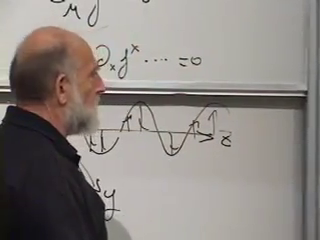
\includegraphics[width=0.70\textwidth]{lecture_58_figure_05.png}
\caption{الرسم التخطيطي المكتمل على السبورة لموجة كهرومغناطيسية عرضية: اهتزازا المجالين الكهربائي والمغناطيسي متعامدان أحدهما على الآخر وعلى اتجاه الانتشار.}
\lectureframe{01:05:25}
\end{figure}

\begin{figure}[H]
\centering
\scalebox{0.90}{%
\begin{tikzpicture}[x=1cm,y=1cm,>=Latex]
  \draw[->,thick] (0,0) -- (8.2,0) node[right] {$z$};
  \draw[->,thick] (0,-1.6) -- (0,1.7) node[above] {$x$};
  \draw[->,thick] (0,0) -- (-1.15,-0.8) node[below left] {$y$};
  \draw[blue!70!black,thick,domain=0:7.5,samples=120]
    plot (\x,{0.95*sin(90*\x)});
  \foreach \z/\s in {0.8/1,2.8/-1,4.8/1,6.8/-1}{
    \draw[->,green!45!black,thick]
      (\z,0) -- ++({-0.55*\s},{-0.38*\s});
  }
  \node[blue!70!black] at (6.9,1.25) {$\mathbf E$};
  \node[green!45!black] at (5.2,-1.05) {$\mathbf B$};
  \draw[->,very thick] (6.2,1.55) -- (7.7,1.55)
    node[midway,above] {propagation};
\end{tikzpicture}
}
\caption{المجالان \(\mathbf E\) و\(\mathbf B\) متعامدان أحدهما على الآخر وعلى اتجاه الانتشار.}
\end{figure}

هذه هي طبيعة الضوء وجميع الإشعاعات الكهرومغناطيسية في الفراغ. وبما أن المعادلات التي أنتجت الموجة متغايرة لورنتزيًا، فإن راصدًا قصوريًا آخر يصف بدوره موجة كهرومغناطيسية تتحرك بسرعة \(c\)، ذات مجالين كهربائي ومغناطيسي عرضيين.

\section{كثافة الشحنة وكثافة التيار}

نعيد الآن المصادر التي تُركت جانبًا مؤقتًا. عندما تشغل جسيمات مشحونة كثيرة منطقة ما، يكون من المفيد تمثيلها تمثيلًا خشنًا في صورة كثافة شحنة مستمرة
\begin{equation}
\rho(\mathbf x,t)=\frac{dQ}{dV}.
\end{equation}
وهذا التقريب يشبه معاملة الماء بوصفه مائعًا مستمرًا رغم أنه يتكوّن من جزيئات. وتسهم الشحنات الموجبة والسالبة بإشارتين متعاكستين، لذا فإن \(\rho\) هي الشحنة الصافية لكل وحدة حجم.

الشحنة في منطقة مختارة \(V\) هي
\begin{equation}
Q_V(t)=\int_V\rho(\mathbf x,t)\,dV.
\label{eq:charge-volume}
\end{equation}
وقد تتغير الكثافة مع الموضع والزمن. يمكن لتجمع من الشحنة أن يتحرك بعيدًا عن نقطة ما، فيغيّر الكثافة الموضعية هناك. لكنها لا يمكن، مع ذلك، أن تتغير على نحو اعتباطي. فالطبيعة تصون الشحنة الكهربائية.

إن الانحفاظ الكلي وحده أضعف من اللازم. إذ سيسمح للشحنة بأن تختفي من الأرض وتظهر من جديد على المريخ في اللحظة نفسها مع بقاء المجموع الكلي من دون تغيير. والعبارة الأقوى محلية: لا يمكن للشحنة أن تغادر موضعًا وتصل إلى آخر إلا عبر تدفق في الفضاء الواقع بينهما.

لوصف ذلك التدفق، خذ عنصر مساحة موجهًا متناهي الصغر
\begin{equation}
d\boldsymbol\sigma=\widehat{\mathbf n}\,d\sigma.
\end{equation}
مقداره هو المساحة، واتجاهه عمودي على السطح. وتُعرَّف كثافة التيار \(\mathbf J\) بحيث تكون الشحنة التي تعبر هذا العنصر في وحدة الزمن هي
\begin{equation}
\frac{dQ}{dt}=\mathbf J\cdot d\boldsymbol\sigma.
\label{eq:current-flux-element}
\end{equation}
ومقدار \(\mathbf J\) هو شحنة لكل وحدة مساحة ولكل وحدة زمن، واتجاهه هو اتجاه سريان الشحنة الموجبة.

\begin{figure}[H]
\centering
\includegraphics[width=0.64\textwidth]{lecture_58_figure_10.png}
\caption{عنصر مساحة موجه وعامل الفيض \(d\boldsymbol\sigma\cdot\mathbf J\).}
\lectureframe{01:18:15}
\end{figure}

يختار الجداء النقطي المركبة العمودية على السطح. فالتيار المماس للسطح لا يعبر أيًّا من الجانبين ويسهم بصفر. والتيار الموازي للعمودي يعطي أقصى فيض لمقدار ثابت. وتيار السلك حالة خاصة واحدة، لكن \(\mathbf J\) قد يصف أيضًا شحنة تتدفق عبر صفيحة أو في كامل الفضاء الثلاثي الأبعاد.

\section{الانحفاظ الموضعي ومعادلة الاستمرارية}

ثبّت منطقة \(V\) في الفضاء، ووجّه كل عنصر من حدودها المغلقة \(\partial V\) نحو الخارج. إذا كان هناك تيار صافٍ إلى الخارج، فإن الشحنة في الداخل تتناقص:
\begin{equation}
\frac{dQ_V}{dt}
=-\oint_{\partial V}\mathbf J\cdot d\boldsymbol\sigma.
\label{eq:integral-conservation}
\end{equation}
إن إشارة السالب هنا فيزيائية لا اصطلاحية: فالفيض الموجب إلى الخارج يزيل شحنة موجبة من المنطقة. وباستخدام المعادلة~\eqref{eq:charge-volume}،
\begin{equation}
\int_V\partial_t\rho\,dV
=-\oint_{\partial V}\mathbf J\cdot d\boldsymbol\sigma.
\label{eq:integral-continuity-one}
\end{equation}

\begin{figure}[H]
\centering
\includegraphics[width=0.72\textwidth]{lecture_58_figure_11.png}
\caption{قانون الانحفاظ لمنطقة ثابتة بعد تحويل فيض السطح إلى صيغة حجمية.}
\lectureframe{01:29:00}
\end{figure}

تربط مبرهنة غاوس، التي تُسمى أيضًا مبرهنة التباعد، بين الفيض عبر سطح مغلق والتباعد في داخله:
\begin{equation}
\oint_{\partial V}\mathbf A\cdot d\boldsymbol\sigma
=\int_V\boldsymbol\nabla\cdot\mathbf A\,dV.
\label{eq:divergence-theorem}
\end{equation}
يمكن تخيل أنابيب خفية تحقن الماء عند نقاط داخل وعاء. يقيس التباعد المعدل الموضعي الذي يخرج به الماء من نهايات الأنابيب؛ ويقيس التكامل السطحي مجموع الماء المغادر للوعاء. وكل ما يُنشأ في الداخل على هيئة تدفق إلى الخارج لا بد أن يعبر الحد في النهاية.

يعطي تطبيق المعادلة~\eqref{eq:divergence-theorem} على \(\mathbf J\)
\begin{equation}
\int_V
\left(\partial_t\rho+\boldsymbol\nabla\cdot\mathbf J\right)dV=0.
\end{equation}
وتسري هذه العلاقة على كل منطقة ممكنة \(V\). لذلك لا بد أن ينعدم المقدار تحت إشارة التكامل نقطةً نقطة:
\begin{equation}
\boxed{\partial_t\rho+\boldsymbol\nabla\cdot\mathbf J=0.}
\label{eq:continuity-three}
\end{equation}

\begin{figure}[H]
\centering
\includegraphics[width=0.72\textwidth]{lecture_58_figure_12.png}
\caption{معادلة الاستمرارية الموضعية مكتوبة مركبةً فمركبة.}
\lectureframe{01:29:50}
\end{figure}

تقول المعادلة~\eqref{eq:continuity-three} بالضبط ما يتطلبه الانحفاظ الموضعي. فإذا انخفضت كثافة الشحنة عند نقطة أو داخل منطقة صغيرة، فلا بد أن يتباعد التيار إلى الخارج منها. وإذا تقارب التيار إلى الداخل، ازدادت كثافة الشحنة.

تكوِّن الكثافة والتيار على نحو طبيعي التيار الرباعي
\begin{equation}
J^\mu=(\rho,J_x,J_y,J_z)
\label{eq:four-current}
\end{equation}
في وحدات \(c=1\). وتصبح معادلة الاستمرارية المعادلة القياسية اللورنتزية
\begin{equation}
\partial_\mu J^\mu=0.
\label{eq:continuity-four}
\end{equation}
وينبغي أن يتحول تدفق توزيع نسبوي كمتجه رباعي، تمامًا كما تفعل السرعة الرباعية لجسيم واحد. وتجعل المعادلة~\eqref{eq:continuity-four} انحفاظ الشحنة الموضعي صحيحًا في كل إطار قصوري.

\section{معادلات ماكسويل مع المصادر}

بإعادة إدخال الشحنة والتيار نحصل على
\begin{align}
\boldsymbol\nabla\cdot\mathbf E&=\rho,
\label{eq:gauss-e-source}\\
\boldsymbol\nabla\cdot\mathbf B&=0,\\
\boldsymbol\nabla\times\mathbf E&=-\partial_t\mathbf B,\\
\boldsymbol\nabla\times\mathbf B&=\partial_t\mathbf E+\mathbf J.
\label{eq:ampere-source}
\end{align}
وتُختزل المعادلات التي تتضمن مصادر كهربائية إلى
\begin{equation}
\boxed{\partial_\mu F^{\mu\nu}=J^\nu,}
\label{eq:maxwell-source-covariant}
\end{equation}
بينما يبقى الزوج المغناطيسي الخالي من المصادر
\begin{equation}
\boxed{\partial_\mu\widetilde F^{\mu\nu}=0.}
\label{eq:maxwell-dual-source}
\end{equation}

\begin{figure}[H]
\centering
\includegraphics[width=0.78\textwidth]{lecture_58_figure_13.png}
\caption{معادلات ماكسويل مع المصادر إلى جانب صيغتها التغايرية \(\partial_\mu F^{\mu\nu}=J^\nu\).}
\lectureframe{01:34:00}
\end{figure}

المركبة الزمنية من المعادلة~\eqref{eq:maxwell-source-covariant} هي
\begin{equation}
\partial_\mu F^{\mu t}=J^t=\rho,
\end{equation}
والحساب بالمركبات الذي أُجري بالفعل يحوّل طرفها الأيسر إلى
\(\boldsymbol\nabla\cdot\mathbf E\). أما المركبات المكانية الثلاث فتعيد إنتاج
\(\boldsymbol\nabla\times\mathbf B=\partial_t\mathbf E+\mathbf J\).

وهناك أيضًا فحص اتساق مفيد. إن تطبيق \(\partial_\nu\) على
المعادلة~\eqref{eq:maxwell-source-covariant} يعطي
\begin{equation}
\partial_\nu J^\nu
=\partial_\nu\partial_\mu F^{\mu\nu}=0,
\end{equation}
وذلك لأن المشتقتين متناظرتان تحت \(\mu\leftrightarrow\nu\)، في حين أن \(F^{\mu\nu}\) مضادّ التناظر.\editorialnote{ينتج فحص الاتساق القصير هذا من المعادلة التغايرية، ويُظهر صراحةً لماذا تحترم معادلات ماكسويل مع المصادر معادلة الاستمرارية تلقائيًا.}

لقد اكتملت الآن البنية التبادلية. يصف قانون القوة الموترية
\(f^\mu=qF^\mu{}_\nu u^\nu\) كيف تؤثر الحقول في الشحنة، وتصف
المعادلة~\eqref{eq:maxwell-source-covariant} كيف تولِّد الشحنة والتيار الحقول. وكلتاهما معادلتان موتريتان. وفي الفراغ، تُنتج معادلات الحقل نفسها موجات مستعرضة تتحرك بسرعة \(c\). ولذلك تلتقي تغايرية لورنتز ومعادلة الموجة الكهرومغناطيسية عند النقطة التي حفَّزت هذا البناء: فكل راصد قصوري يجد القوانين نفسها للكهرومغناطيسية والسرعة نفسها للضوء.
\chapter{الزمن الخاص، وتمدد الزمن، وانكماش الطول}

سنختار كثيرًا وحدات تكون فيها سرعة الضوء $c=1$. في تلك الوحدات يمكن مقارنة سنة من الزمن وسنة ضوئية من المسافة مباشرةً، وتصبح الصيغ أسهل بكثير في القراءة. وكلما كانت $c$ ذات أهمية فيزيائية، أعدنا إدراجها. ويكفي التحليل البعدي لتحديد موضعها.

\section{شبكة الزمكان الغاليلي}

ابدأ بالعلاقة السابقة لأينشتاين بين إطار ساكن وقطار يتحرك بسرعة $v$ على طول محور $x$:
\begin{align}
x' &= x-vt, & t'&=t.
\label{eq:l4-galilean}
\end{align}
تتضمن المعادلة الثانية افتراض نيوتن بوجود زمن كوني. فكل راصد يستخدم شرائح التزامن نفسها، مع أن أصول الإحداثيات المكانية تتحرك بعضها بالنسبة إلى بعض.

افترض أن الراصد في الإطار غير المعلَّم بشرطة يقف بجانب السكة، وأن الراصد في الإطار المعلَّم بشرطة يركب القطار. يحقق أصل القطار $x'=0$، لذا فإن خط عالمه في الإحداثيات غير المعلَّمة بشرطة هو
\begin{equation}
x=vt.
\end{equation}
وذلك الخط المائل هو محور $t'$. وعلى النقيض من ذلك، فإن $t'=t$ تعني أن جميع الخطوط ذات $t'$ الثابت هي الخطوط الأفقية نفسها ذات $t$ الثابت.

\begin{figure}[H]
\centering
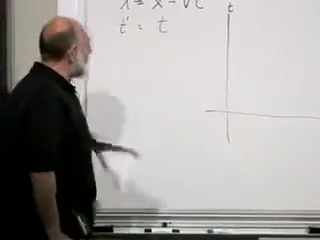
\includegraphics[width=0.72\textwidth]{lecture_04_figure_02.png}
\caption{التحويل الغاليلي وشبكة $t$-$x$ الابتدائية. سيتتبع الأصل المتحرك $x=vt$، بينما يحتفظ الإطاران بخطوط مشتركة للزمن الثابت.}
\lectureframe{00:03:06}
\end{figure}

بحل المعادلة ~\eqref{eq:l4-galilean} بالنسبة إلى الإحداثيات غير المعلَّمة بشرطة نحصل على
\begin{align}
x&=x'+vt'=x'+vt, & t&=t'.
\end{align}
وللمعكوس الصيغة نفسها مع استبدال $v$ بـ $-v$. فإذا كان القطار يتحرك إلى الأمام بالنسبة إلى المحطة، فإن المحطة تتحرك إلى الخلف بالنسبة إلى القطار. وتبقى هذه التبادلية قائمة في النسبية الخاصة، لكن الزمن الكوني لا يبقى.

\section{تصحيح لورنتز}

لا تستطيع التحويلات الغاليليّة أن تجعل سرعة الضوء واحدة في كل إطار قصوري. والعلاقات المصححة هي، أولًا في وحدات $c=1$،
\begin{align}
x'&=\frac{x-vt}{\sqrt{1-v^2}}, &
t'&=\frac{t-vx}{\sqrt{1-v^2}}.
\label{eq:l4-lorentz-natural}
\end{align}
وبإعادة الوحدات المعتادة نحصل على
\begin{align}
x'&=\frac{x-vt}{\sqrt{1-v^2/c^2}}, &
t'&=\frac{t-vx/c^2}{\sqrt{1-v^2/c^2}}.
\label{eq:l4-lorentz-c}
\end{align}

\begin{figure}[H]
\centering
\includegraphics[width=0.74\textwidth]{lecture_04_figure_05.png}
\caption{تحويل لورنتز مع إعادة عوامل $c$.}
\lectureframe{00:09:10}
\end{figure}

عندما يكون $v\ll c$، يكون كل من $v^2/c^2$ و $vx/c^2$ صغيرًا جدًا في الظروف التي تُستخدم فيها الميكانيكا النيوتنية. وعندئذٍ تختزل المعادلة ~\eqref{eq:l4-lorentz-c} إلى النتيجة الغاليليّة. فالنسبية لا تلغي حركيات نيوتن؛ بل تحدد مجال صلاحيتها.

عند $v=c$، ينعدم المقام. ولا يمكن لإطار قصوري أن يتحرك بسرعة الضوء بالنسبة إلى إطار قصوري آخر. ودون ذلك الحد بكثير تكون التصحيحات صغيرة، ولكن بالقرب منه يصبح امتزاج $x$ و $t$ أمرًا لا مفر منه.

اختيرت الحركة على طول $x$، لذا لا تتغير الإحداثيات المستعرضة:
\begin{equation}
y'=y,\qquad z'=z.
\end{equation}
ومن طرائق فهم السبب وضع قضبان مترية مستعرضة متطابقة على القطار وعلى الرصيف. فالراصد الذي يتحرك بسرعة وسطية بين الإطارين يرى القضبان تقترب بسرعات متساوية ومتعاكسة. ولا تتضمن هذه الهيئة أي سمة يمكن أن تجعل أحد القضيبين المستعرضين أقصر من الآخر.

\section{تحويلات لورنتز على امتداد مخروط الضوء}

توجد طريقة هندسية لقراءة المعادلة ~\eqref{eq:l4-lorentz-natural}. اجمع معادلتيها:
\begin{align}
t'+x'
&=\frac{(t-vx)+(x-vt)}{\sqrt{1-v^2}}\\
&=(t+x)\frac{1-v}{\sqrt{1-v^2}}\\
&=(t+x)\sqrt{\frac{1-v}{1+v}}.
\label{eq:l4-null-plus}
\end{align}
واطرح إحداهما من الأخرى بالترتيب المتمم:
\begin{align}
t'-x'
&=\frac{(t-vx)-(x-vt)}{\sqrt{1-v^2}}\\
&=(t-x)\frac{1+v}{\sqrt{1-v^2}}\\
&=(t-x)\sqrt{\frac{1+v}{1-v}}.
\label{eq:l4-null-minus}
\end{align}

\begin{figure}[H]
\centering
\includegraphics[width=0.75\textwidth]{lecture_04_figure_06.png}
\caption{تحويل لورنتز بعد إعادة كتابته بالتركيبين العدميين
$t+x$ و $t-x$. وعاملا المقياس فيهما متبادلان عكسيًا.}
\lectureframe{00:18:45}
\end{figure}

التركيبان $t+x$ و $t-x$ هما إحداثيان على امتداد الاتجاهين الضوئيين عند $45^\circ$. يضغط التحويل الدفعي أحد هذين الاتجاهين ويمد الآخر بالعامل العكسي. وهو لا يدير أيًّا منهما بعيدًا عن $45^\circ$. وهكذا تبقى الأشعة الضوئية أشعةً ضوئية، وهذه هي الصورة الزمكانية لثبات سرعة الضوء.

\begin{classroomqa}
\audiencequestion{يرى الراصد في الإطار المتوسط تجربةً متناظرة، ولكن كيف يثبت ذلك النتيجة لراصدي القطار والرصيف؟
\lecturetimestamp{00:20:48}}
\lecturerresponse{يُستخدم هنا أمر إضافي واحد: إن تلاقي الأحداث ثابت. فإذا التقت أطراف القضبان، كان ذلك التلاقي حدثًا زمكانيًا واحدًا. ويجوز لكل راصد قصوري أن يعيّن له إحداثيات مختلفة، ولكن لا يجوز لأي منهم أن يقسم تلاقيًا واحدًا إلى موضعين مختلفين. والومضات المنبعثة عند التقاء النهايات المتناظرة تجعل هذه الأحداث قابلة للكشف عمليًا. ومن ثم يثبت تناظر الإطار المتوسط وثبات تلاقيي النهايتين أن الأطوال المستعرضة متساوية.}
\end{classroomqa}

\begin{classroomqa}
\audiencequestion{هل يجب أن يكون راكب الدراجة الذي يمثّل الإطار المتوسط موجودًا ماديًا عند منتصف القضبان؟\lecturetimestamp{00:22:25}}
\lecturerresponse{لا. فالإطار المرجعي شبكة كاملة من الراصدين والساعات، لا عينًا واحدة في موضع واحد. وقد يتلقى راكب الدراجة ومضات النهايات لاحقًا ويستدل على مواضع انبعاثها. وما يهم هو الموضع الزمكاني لكل حدث انبعاث، لا الموضع الذي يُستقبل فيه الضوء في نهاية الأمر.}
\end{classroomqa}

إن تركيب السرعات المتعاقبة نتيجة أخرى للتحويل نفسه، لكنه يُترك عمدًا للمحاضرة التالية. أما المهمة الحالية فهي تحديد الكمية الثابتة التي تقيسها ساعة متحركة.

\section{الفاصل الثابت}

في دوران المحاور الديكارتية العادية، تبقى الكمية $x^2+y^2$ دون تغير. وتحفظ تحويلات لورنتز صيغةً تربيعية مختلفة. فمن المعادلة ~\eqref{eq:l4-lorentz-natural}،
\begin{align}
t'^2-x'^2
&=\frac{(t-vx)^2-(x-vt)^2}{1-v^2}\\
&=\frac{t^2-2vtx+v^2x^2-x^2+2vtx-v^2t^2}{1-v^2}\\
&=t^2-x^2.
\label{eq:l4-interval}
\end{align}
تتلاشى الحدود المختلطة، ويحتوي البسط المتبقي على عامل مشترك هو $1-v^2$.

\begin{figure}[H]
\centering
\includegraphics[width=0.76\textwidth]{lecture_04_figure_07.png}
\caption{الاشتقاق على السبورة لـ $t'^2-x'^2=t^2-x^2$.}
\lectureframe{00:33:15}
\end{figure}

مع ثلاثة أبعاد مكانية يكون الثابت هو
\begin{equation}
t'^2-x'^2-y'^2-z'^2=t^2-x^2-y^2-z^2
\end{equation}
في وحدات $c=1$. وعلى نحو أعم، نستخدم فروق الإحداثيات بين حدثين:
\begin{equation}
\Delta s^2
=c^2\Delta t^2-\Delta x^2-\Delta y^2-\Delta z^2.
\label{eq:l4-spacetime-interval}
\end{equation}
ويتفق كل راصد قصوري على هذا العدد، رغم أنهم يختلفون في حدوده المنفصلة للزمان والمكان.

\section{الزمن الخاص والساعات المتحركة}

تخيّل شبكةً من الراصدين الساكنين جرت مزامنة ساعاتهم بتبادل إشارات ضوئية. وتحدد قراءاتهم الزمن الإحداثي $t$. والآن احمل ساعة يد واحدة عبر تلك الشبكة. فقراءتها الخاصة ترافق الساعة على طول خط عالمها؛ وتلك القراءة هي الزمن الخاص.

لحدثين يفصل بينهما فاصل زمني، عرّف
\begin{equation}
c^2\Delta\tau^2
=c^2\Delta t^2-\Delta x^2-\Delta y^2-\Delta z^2.
\label{eq:l4-proper-time}
\end{equation}
وفي بعد مكاني واحد مع $c=1$، يصبح هذا ببساطة
\begin{equation}
\Delta\tau=\sqrt{\Delta t^2-\Delta x^2}.
\end{equation}
ويوازي الجذر التربيعي الصيغة الخاصة بالمسافة العادية، لكن الإشارة السالبة تغيّر الهندسة.

توجد ثلاث حالات:
\begin{align}
\Delta t^2-\Delta x^2 &>0 &&\text{timelike},\\
\Delta t^2-\Delta x^2 &=0 &&\text{lightlike},\\
\Delta t^2-\Delta x^2 &<0 &&\text{spacelike}.
\end{align}
داخل مخروط الضوء يكون الزمن الخاص حقيقيًا. وعلى المخروط، حيث $x=\pm t$، يكون صفرًا رغم أن الحدثين لا يلزم أن يتطابقا. ويمكن لشعاع ضوئي أن يصل بين مثل هذه الأحداث على وجه الدقة. وخارج المخروط يكون الفصل مكانيًا؛ ومن الأفضل وصفه بالمسافة الخاصة الحقيقية $\sqrt{\Delta x^2-\Delta t^2}$ بدلًا من زمن ساعة تخيلي.

\begin{figure}[H]
\centering
\includegraphics[width=0.73\textwidth]{lecture_04_figure_08.png}

\vspace{0.8em}

\begin{tikzpicture}[x=1.0cm,y=1.0cm]
\draw[->] (-3.3,0) -- (3.3,0) node[right] {$x$};
\draw[->] (0,-0.4) -- (0,4.0) node[above] {$t$};
\draw[thick] (0,0) -- (3.0,3.0) node[above right] {$x=t$};
\draw[thick] (0,0) -- (-3.0,3.0) node[above left] {$x=-t$};
\node at (0,2.0) {timelike};
\node at (2.25,1.05) {spacelike};
\node at (-2.25,1.05) {spacelike};
\end{tikzpicture}
\caption{مخروط الضوء على السبورة وتصنيف واضح للفصل الزمني، والضوئي، والمكاني.}
\lectureframe{00:38:40}
\end{figure}

لماذا تساوي المعادلة ~\eqref{eq:l4-proper-time} قراءةَ ساعة؟ بالنسبة إلى ساعة ساكنة، يكون $\Delta x=0$، ومن ثم $\Delta\tau=\Delta t$. وبالنسبة إلى ساعة تتحرك حركة منتظمة، اختر الإطار المعلَّم بشرطة الذي تكون فيه تلك الساعة ساكنة. هناك يكون $\Delta x'=0$، ويعطي الثبات
\begin{equation}
\Delta\tau
=\sqrt{\Delta t'^2-\Delta x'^2}
=\Delta t'.
\end{equation}
ولذلك تعدّ الساعات المتحركة الزمن الخاص.

\begin{classroomqa}
\audiencequestion{هل يُستعمل ``الفاصل بين الحدثين'' و ``قراءة الساعة'' بوصفهما اسمين للشيء نفسه؟
\lecturetimestamp{00:44:49}}
\lecturerresponse{يتطابقان عندما تنتقل ساعة مثالية قصوريًا من أحد الحدثين إلى الآخر. فالفاصل الثابت كمية هندسية؛ أما الفرق بين قراءتي الطرفين للساعة المصاحبة للحركة فهو قياسه الفيزيائي. وعادةً ما تسجل ساعة إحداثية ساكنة فاصلًا مختلفًا للزمن الإحداثي.}
\end{classroomqa}

\section{تمدد الزمن والتزامن}

انظر إلى أصل الإطار المتحرك. يحقق خط عالمه
\begin{equation}
x'=0,\qquad x=vt.
\end{equation}
والخط المائل نفسه هو في آن واحد مسار الساعة المتحركة ومحور $t'$.

\begin{figure}[H]
\centering
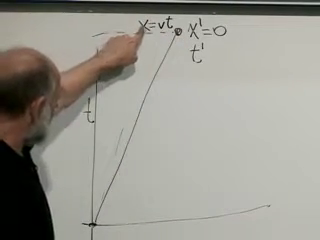
\includegraphics[width=0.72\textwidth]{lecture_04_figure_03.png}
\caption{الأصل المتحرك: $x=vt$، و$x'=0$، ومحور $t'$ هي ثلاثة أوصاف لخط العالم نفسه.}
\lectureframe{00:48:18}
\end{figure}

طبّق الفاصل الثابت بين الأصل المشترك ونقطة لاحقة على ذلك الخط العالمي:
\begin{align}
t'^2-x'^2&=t^2-x^2,\\
t'^2&=t^2-v^2t^2,\\
t'&=t\sqrt{1-v^2}.
\label{eq:l4-time-dilation-natural}
\end{align}
ومع إعادة $c$ نحصل على
\begin{equation}
\Delta\tau=\Delta t\sqrt{1-\frac{v^2}{c^2}}
=\frac{\Delta t}{\gamma},
\qquad
\gamma=\frac{1}{\sqrt{1-v^2/c^2}}.
\label{eq:l4-time-dilation}
\end{equation}

\begin{figure}[H]
\centering
\includegraphics[width=0.73\textwidth]{lecture_04_figure_09.png}
\caption{نتيجة تمدد الزمن على السبورة: يتراكم على الساعة المتحركة $t'=t\sqrt{1-v^2}$ في وحدات يكون فيها $c=1$.}
\lectureframe{00:50:45}
\end{figure}

يقول الراصد الساكن إن الساعة المتحركة تسير ببطء. وتقتضي المعاملة بالمثل أن يقول الراصد المتحرك الشيء نفسه عن الساعات الساكنة. ولا يوجد تناقض، لأن الوصفين يقارنان زوجين مختلفين من الأحداث المتباعدة.

في الواقع، إذا كانت قيمة $t'$ ثابتة في المعادلة ~\eqref{eq:l4-lorentz-natural}، فإن ذلك يقتضي
\begin{equation}
t-vx=\text{constant}.
\label{eq:l4-simultaneity}
\end{equation}
خطوط التزامن لدى الراصد المتحرك مائلة بالنسبة إلى الخطوط الأفقية $t=\text{constant}$. ويعدّ كل راصد مجموعة مختلفة من قراءات الساعات المتباعدة متزامنة. ومتى أُبقي هذا الاختلاف ظاهرًا، اتسق التباطؤ المتبادل للساعات.

\begin{figure}[H]
\centering
\begin{tikzpicture}[x=1cm,y=1cm]
\draw[->] (0,0) -- (0,4.2) node[above] {$t$};
\draw[->] (0,0) -- (5.2,0) node[right] {$x$};
\draw[thick,->] (0,0) -- (2.4,3.8) node[above] {$x'=0$};
\draw[dashed] (0,2.8) -- (4.8,2.8)
  node[right] {$t=\mathrm{const}$};
\draw[thick] (0.15,1.05) -- (4.7,2.35)
  node[right] {$t'=\mathrm{const}$};
\draw[thick] (3.4,0) -- (3.4,3.8);
\fill (3.4,2.8) circle (0.045);
\fill (3.4,1.98) circle (0.045);
\end{tikzpicture}
\caption{يقارن تمدد الزمن المتبادل قراءات الساعات على شرائح تزامن مختلفة.}
\end{figure}

\section{مسارا التوأمين}

يبدأ توأمان من الحدث نفسه. يبقى أحدهما عند $x=0$. ويسافر الآخر مبتعدًا بسرعة $v$، ثم يعكس اتجاهه ويعود بالسرعة نفسها. وعندما يلتقيان من جديد يقارنان كل عملية فيزيائية يمكن أن تصلح ساعةً: ساعات اليد، وخفقات القلب، والأيض، أو حتى الشيخوخة نفسها.

لنفترض أن كل نصف من الرحلة يستغرق زمنًا إحداثيًا مقداره $T$ في إطار التوأم المقيم. يكون الزمن الخاص للتوأم المقيم
\begin{equation}
\tau_{\mathrm{home}}=2T.
\end{equation}
وإحداثيا حدث الانعطاف هما $(vT,T)$. ولذلك تسهم المرحلة الأولى من الرحلة بمقدار
\begin{align}
\tau_{\mathrm{leg}}
&=\sqrt{T^2-v^2T^2}
=T\sqrt{1-v^2}.
\end{align}
وتسهم مرحلة الإياب بالمقدار نفسه، ومن ثم
\begin{equation}
\tau_{\mathrm{travel}}=2T\sqrt{1-v^2}<2T.
\label{eq:l4-twin}
\end{equation}

\begin{figure}[H]
\centering
\includegraphics[width=0.73\textwidth]{lecture_04_figure_10.png}

\vspace{0.8em}

\begin{tikzpicture}[x=1.1cm,y=1cm]
\draw[->] (-0.2,0) -- (3.4,0) node[right] {$x$};
\draw[->] (0,-0.1) -- (0,4.4) node[above] {$t$};
\draw[very thick] (0,0) -- (0,4);
\draw[very thick] (0,0) -- (2.2,2) -- (0,4);
\draw[dashed] (0,2) -- (2.2,2);
\node[left] at (0,2) {$T$};
\node[left] at (0,4) {$2T$};
\node[below right] at (1.1,1.0) {$v$};
\node[above right] at (1.1,3.0) {$-v$};
\end{tikzpicture}
\caption{خط العالم للتوأم المقيم ومرحلتا الرحلة. أزمنتها الخاصة مختلفة لأنها مسارات مختلفة عبر الزمكان.}
\lectureframe{00:59:35}
\end{figure}

لا يوجد تناقض في عدم تساوي العمرين. فمسار الرحلة يتضمن انعطافًا، ولا يرتبط بالمسار المستقيم للتوأم المقيم بتناظر واحد لإطار قصوري. وفي الهندسة الإقليدية العادية يكون أيضًا للمسار المستقيم والمسار المنكسر بين نقطتين طولان مختلفان. وتعكس هندسة مينكوفسكي أيَّ المسارين له الفاصل الأكبر، لكن المقارنة تظل هندسية.

\section{التسارع والساعة المثالية}

\begin{classroomqa}
\audiencequestion{عند الانعطاف تكون الفيزياء مختلفة ويتسارع المسافر. فهل يُبطل ذلك حساب الساعة؟
\lecturetimestamp{01:02:19}}
\lecturerresponse{التسارع حقيقي ويساعد على تحديد عدم التناظر؛ ولا ينبغي محاولة التخلص منه بالمجادلة. والزاوية الحادة ليست إلا تمثيلًا مثاليًا، ويمكن استبدالها بانعطاف ذي مدة منتهية. والافتراض الفيزيائي الإضافي هو أن الساعة، إذا كانت صغيرة بما يكفي ومحكمة الصنع، تكون غير حساسة لتسارع معتدل وتستمر في تسجيل الزمن الخاص. وقد تتشوه ساعة كبيرة أو هشة أو تنكسر، لكن ذلك عيب في الآلية لا في الفاصل الزمكاني.}
\end{classroomqa}

هذا الافتراض الخاص بالساعة المثالية لا يُستمد من تحويل لورنتز وحده. بل يُختبَر من خلال سلوك آليات الساعات الفعلية. وتُعد الذرة تقريبًا أفضل بكثير من ساعة يبلغ عرضها مئات الأميال، لأن الآلية المدمجة أشد مقاومة للتشوه تحت تأثير التسارع أو الجاذبية. وإن استحضار النسبية العامة بالاسم لن يزيل هذه المسألة الفيزيائية؛ إذ سيظل لا بد من معرفة كيف تستجيب الآلية المختارة لبيئتها.

\begin{classroomqa}
\audiencequestion{هل يمكن تجزئة مسار متسارع إلى فترات قصيرة يبقى فيها التحليل القصوري صالحًا؟\lecturetimestamp{01:09:08}}
\lecturerresponse{نعم. قسِّم المنحنى إلى مقاطع قصيرة تكاد تكون مستقيمة، واحسب الزمن الخاص على كل مقطع، ثم اجمع النتائج. وهذا هو النظير الزمكاني لإيجاد طول منحنى عادي من كثير من القطع المستقيمة الصغيرة. وفي حد المتصل،
\[
\tau=\int \sqrt{1-\frac{v(t)^2}{c^2}}\,dt,
\]
وذلك لحركة في زمكان مستوٍ موصوفة في نظام إحداثيات قصوري.}
\end{classroomqa}

\section{ما يراه التوأمان}

يمكن جعل القراءات النهائية للساعتين إجرائيةً بإرسال نبضات ضوئية. علِّم فواصل مقدار كل منها ثانية واحدة من الزمن الخاص على خطي العالم كليهما، ودَع كل توأم يطلق نبضة عند كل علامة. أثناء مرحلة الابتعاد، تصل النبضات الواردة من التوأم الآخر متباعدة. وأثناء العودة، تصل متقاربة. وهذا هو تأثير دوبلر النسبي معبَّرًا عنه مباشرةً على مخطط الزمكان.

\begin{figure}[H]
\centering
\includegraphics[width=0.73\textwidth]{lecture_04_figure_11.png}
\caption{الإشارات الضوئية المتبادلة بين خط العالم للمقيم وخط العالم للمسافر. فالتباعد في وصولها في مرحلة الابتعاد والتقارب في وصولها في مرحلة العودة يفسران جميع النبضات المنبعثة.}
\lectureframe{01:12:55}
\end{figure}

لا يختفي أي إطار مرجعي في هذا الوصف. فكل راصد يتلقى في نهاية المطاف جميع النبضات التي يبعثها الآخر، لكن معدلات استقبالها تعتمد على الحركة النسبية. والانزياح الأحمر في مرحلة الابتعاد والانزياح الأزرق في مرحلة العودة ليسا تأثيرين متساويي المدة على المسارين، لذا فإن عدَّ جميع النبضات المستقبلة يتفق مع مقارنة الزمن الخاص.

\begin{classroomqa}
\audiencequestion{إذا كان المسافر العائد يستقبل ضوءًا منزاحًا نحو الأزرق، أفيمكنه أن يتلقى طاقةً أكثر مما أصدره المصدر؟
\lecturetimestamp{01:13:50}}
\lecturerresponse{يتطلب ذلك السؤال تعريف الطاقة في النسبية واعتمادها على الإطار المرجعي، وهو ما لم نطوره بعد. وهذا سؤال معقول، لكن الإحداثيات وعدَّ النبضات وحدهما لا يكفيان لتسوية حسابات الطاقة، ولا سيما بالنسبة إلى راصد متسارع. لذلك ينبغي تأجيل الجواب بدلًا من تخمينه.}
\end{classroomqa}

\section{اتجاه مكاني مضغوط}

\begin{classroomqa}
\audiencequestion{افترض أن أحد الاتجاهات المكانية مضغوط. هل يمكن لأحد التوأمين أن يتحرك بانتظام على امتداده، ويعود إلى موضع البداية، ويتجنب التسارع تمامًا؟ فما الذي يميز التوأمين إذن؟\lecturetimestamp{01:15:14}}
\lecturerresponse{ينبغي أن يُتخيل الفضاء من داخله على أنه أسطوانة، لا صفيحة منحنية داخل فضاء أكبر؛ فلا حاجة إلى أي تسارع شعاعي. ومع ذلك، يواجه الراصد العائد الخاصية العالمية المتمثلة في أن الأمكنة نفسها تتكرر. وهذا يدل على لاتناظر، لكن الجواب الكامل يتطلب معالجة دقيقة للنسبية الخاصة مع التطابق المكاني. ويُترك السؤال هنا مفتوحًا بدلًا من الإجابة عنه ارتجالًا.}
\end{classroomqa}

\begin{figure}[H]
\centering
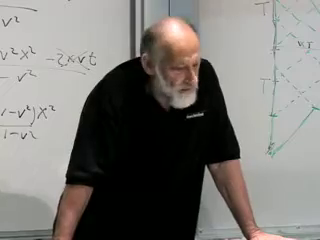
\includegraphics[width=0.72\textwidth]{lecture_04_figure_04.png}

\vspace{0.8em}

\begin{tikzpicture}[x=1cm,y=1cm]
\draw[thick] (0,0) ellipse (1.3 and 0.35);
\draw[thick] (-1.3,0) -- (-1.3,-3.1);
\draw[thick] (1.3,0) -- (1.3,-3.1);
\draw[thick] (0,-3.1) ellipse (1.3 and 0.35);
\draw[->,very thick] (0.0,0.38) arc (90:-210:1.38 and 0.42);
\node[right] at (1.65,-1.5) {compact spatial direction};
\end{tikzpicture}
\caption{مسألة الفضاء المضغوط كما رُسمت على اللوح، مع تمثيل أسطواني جوهري واضح. وهي مسألة تتعلق بالتطابق العالمي، لا بحركة حول أسطوانة مُضمَّنة في بُعد شعاعي إضافي.}
\lectureframe{01:17:56}
\end{figure}

\section{يُقاس الطول على مقطع تزامن}

في مسألة من مسائل النسبية الخاصة، ارسم أولًا مخطط الزمكان. خذ قضيبًا متريًا ساكنًا في الإطار غير المعلَّم بشرطة، وطرفاه عند $x=0$ و$x=1$. ومع مرور الزمن، يرسم الطرفان خطَّي عالم رأسيين. ويكنس القضيب شريطًا بينهما.

يجب على الراصد المتحرك أن يقيس كلا الطرفين عند قيمة واحدة من زمن الإطار المتحرك $t'$. ومن المعادلة ~\eqref{eq:l4-simultaneity}، فإن المقطع المار بالمبدأ الذي فيه $t'=0$ يحقق
\begin{equation}
t=vx
\end{equation}
بوحدات $c=1$. وهو يقطع الطرف الأيمن $x=1$ عند $t=v$.

\begin{figure}[H]
\centering
\includegraphics[width=0.73\textwidth]{lecture_04_figure_12.png}

\vspace{0.8em}

\begin{tikzpicture}[x=1.55cm,y=1.15cm]
\draw[->] (-0.5,0) -- (3.1,0) node[right] {$x$};
\draw[->] (0,0) -- (0,3.8) node[above] {$t$};
\draw[very thick,red] (0,0) -- (0,3.3);
\draw[very thick,red] (2.15,0) -- (2.15,3.3);
\fill[red!12] (0,0) rectangle (2.15,3.3);
\draw[very thick,green!50!black] (0,0) -- (1.2,3.1)
  node[above] {$x=vt$};
\draw[very thick,blue] (0,0) -- (2.15,1.15)
  node[right] {$t'=0$};
\fill (2.15,1.15) circle (0.045);
\node[right] at (2.22,1.35) {$(x,t)=(1,v)$};
\node[below] at (2.15,0) {$1$};
\end{tikzpicture}
\caption{يقوم قضيب ساكن بكنس شريط زمكاني. والطول الذي يقيسه الراصد المتحرك هو المسافة بين طرفيه على مقطع واحد من $t'=\mathrm{const}$.}
\lectureframe{01:24:20}
\end{figure}

الفاصل المختار بين الطرفين شبيه بالمكان، لذا نستخدم الصيغة المكانية الموجبة للمقدار الثابت:
\begin{equation}
x'^2-t'^2=x^2-t^2.
\end{equation}
وعند الطرف المختار، $t'=0$ و$x=1$ و$t=v$. ومن ثم
\begin{align}
x'^2&=1-v^2,\\
x'&=\sqrt{1-v^2}.
\end{align}
إذًا يُقاس طول السكون $L$ في الإطار المتحرك على أنه
\begin{equation}
L'=L\sqrt{1-v^2/c^2}=\frac{L}{\gamma}.
\label{eq:l4-length-contraction}
\end{equation}

\begin{figure}[H]
\centering
\includegraphics[width=0.76\textwidth]{lecture_04_figure_13.png}
\caption{البناء الهندسي المكتمل لانكماش الطول، والنتيجة على اللوح $x'=\sqrt{1-v^2}$ لطول سكوني مقداره وحدة واحدة.}
\lectureframe{01:28:10}
\end{figure}

والعبارة العكسية صحيحة أيضًا: إذ ينسب راصد الرصيف طولًا أقصر إلى القضيب المتري الطولي للقطار. ومرة أخرى، يختار الراصدان حدثين طرفيين متزامنين مختلفين، لذا فالتبادلية ليست متناقضة.

\section{أسئلة في النهاية}

\begin{classroomqa}
\audiencequestion{هل ينتشر شيء غير الضوء بسرعة الضوء؟ وعلى وجه الخصوص، ماذا عن الجاذبية؟\lecturetimestamp{01:29:29}}
\lecturerresponse{تتنبأ النسبية العامة بموجات ثقالية تنتشر بسرعة $c$. وفي وقت هذه المحاضرة، كانت الأدلة تأتي على نحو غير مباشر من أنظمة مثل النجوم النابضة الثنائية؛ ولم تكن الموجات الثقالية قد كُشفت مباشرة بعد.\editorialnote{تغيّر الوضع التجريبي بعد هذه المحاضرة في 2006. فقد رصد LIGO مباشرة GW150914 في 2015، وأظهر الرصد المشترك لـ GW170817 ونظيره الكهرومغناطيسي في 2017 أن سرعتي انتشار الجاذبية والضوء تتفقان ضمن بضع أجزاء في $10^{15}$. انظر \url{https://ligo.org/detections/gw150914/} و\url{https://doi.org/10.1103/PhysRevLett.119.251302}.}}
\end{classroomqa}

\begin{classroomqa}
\audiencequestion{هل يستطيع رائد فضاء أن يقطع مسافة مقدارها سنوات ضوئية كثيرة في زمن خاص أقل من قيمة تلك المسافة عندما تُعبَّر بالسنوات الضوئية؟ وهل يعني ذلك أنه يتحرك أسرع من الضوء؟\lecturetimestamp{01:30:38}}
\lecturerresponse{زمن رائد الفضاء الخاص هو $\sqrt{\Delta t^2-\Delta x^2}$، وهو أصغر من الزمن الإحداثي $\Delta t$. وفي الإطار القصوري لرائد الفضاء، تكون المسافة بين النجمين منكمشة وفق لورنتز. ويتحرك النجمان بسرعة $-v$، لا أسرع من الضوء؛ فثمة ببساطة مسافة منكمشة أقل لقطعها.}
\end{classroomqa}

إذا بدأ رائد الفضاء من السكون ثم تسارع، فإن الوصف يتبدل عبر تعاقب من الأطر القصورية اللحظية. ويمكن أن تتغير المسافة المحسوبة إلى النجوم خلال ذلك الانتقال. ولا يمكن تطبيق تحويل لورنتز ثابت واحد على التاريخ المتسارع بأكمله، لكن الزمن الخاص الكلي يظل يُحسب بجمع المساهمات على طول خط العالم. وينطبق القول نفسه على توأم واقعي ينطلق، وينعطف، ويتباطأ، بدلًا من أن يولد وهو يسير بسرعة الرحلة.

\begin{classroomqa}
\audiencequestion{هل تنشأ هذه الألغاز من معاملة الزمن على أنه مميز؟ وهل يجب أن نسميه بُعدًا رابعًا؟\lecturetimestamp{01:36:43}}
\lecturerresponse{ليس من الضروري أن نبدأ بالشعار القائل إن الزمن بُعد رابع. فتحويل لورنتز نفسه يفرض تداخل المكان والزمان، بينما يعامل الفاصل $t^2-x^2-y^2-z^2$ كليهما بوصفهما جزأين من هندسة واحدة، مع اختلاف الإشارة بين الزمان والمكان. عند السرعات المنخفضة يصبح هذا التداخل مهمَلًا، وتعود الحدوس النيوتونية المألوفة. أما عند السرعات النسبية، فلا يمكن النظر إلى المكان والزمان على أنهما منفصلان انفصالًا جوهريًا.}
\end{classroomqa}

لذلك فإن تمدد الزمن، وانكماش الطول، ومقارنة التوأمين، واختصار زمن الرحلة، ليست حيلًا منفصلة. فهي جميعًا تتبع من ثلاث عادات: تحديد الأحداث الجاري مقارنتها، ورسم هندستها في الزمكان، واستخدام الفاصل الثابت.
\chapter{الكرات النارية، والأطر المرجعية، والمتجهات الرباعية}

نبدأ بسؤال بقي من مناقشة التصادمات عالية الطاقة. فتصادم نواتين ثقيلتين يخلق جسماً يتغير بعنف، لا ثقباً أسود فلكياً هادئاً. فما الذي يمكن أن يعنيه، إذن، وصف هذا التصادم بأفق؟ يقود الجواب عبر صورة خماسية الأبعاد لمادة مقترنة بقوة، ومجموعة من الأسئلة العملية عن المسرّعات، ثم يعود أخيراً إلى هندسة النسبية الخاصة. وبحلول النهاية، تكون السرعة والزخم قد أصبحا متجهين رباعيين، وتكون الطاقة قد أخذت مكانها إلى جانب المركبات الثلاث للزخم.

\section{كرة نارية في بُعد خامس}

\begin{classroomqa}\audiencequestion{الجسم المتولد في التصادم غير مستقر ويتغير شكله. فكيف يمكن تسمية مثل هذا الجسم المعقد ثقباً أسود؟}\lecturerresponse{تخيّل اتجاهاً مكانياً خامساً يمتد بين أرضية وسقف. تجذب الجاذبية في ذلك الاتجاه الاستثارات نحو الأرضية. يودِع التصادم هناك كتلة ساخنة من الطاقة؛ وهذه الكتلة تنتشر ويتغير شكلها، لكنها مع ذلك يمكن أن تمتلك أفقاً ودرجة حرارة وإنتروبيا.}\end{classroomqa}

تخيّل جسيمات، أو على نحو تصويري أكثر أوتاراً صغيرة، تتحرك في هذا العالم الخماسي الأبعاد. فالاستثارات التي تهبط إلى الأرضية تظهر في أربعة أبعاد على هيئة هادرونات: بروتونات ونيوترونات وميزونات وأجسام مركبة ممتدة أخرى. أما الاستثارات المرتبطة بالقرب من السقف فتبدو أكثر أولية. ومن ثم فإن الموضع العمودي طريقة هندسية لترميز المقياس: فالأرضية تمثل النظام الهادروني عند المسافات الطويلة، بينما يمثّل السقف درجات الحرية عند المسافات القصيرة.

عندما يتصادم هادرونان، يصطدم جسمان قرب الأرضية أحدهما بالآخر ويُحدثان تناثراً كبيراً للطاقة. والنتيجة ليست جسماً صلباً. إنها كتلة ساخنة ذات أفق، أشبه ببركة في الحقل الثقالي خماسي الأبعاد. وهي ليست ثقباً أسود فلكياً في الفضاء العادي رباعي الأبعاد، ولا ثقباً أسود على مقياس بلانك ملتصقاً بالسقف. بل هي الوصف الثقالي للكرة النارية شديدة التفاعل قرب الأرضية.

عند الطاقة العالية تنكمش النوى الداخلة انكماش لورنتز إلى أقراص رقيقة. تتصادم، وتودِع طاقتها في منطقة صغيرة، وتنتج مائعاً ينتشر نحو الاتزان. وكانت لزوجته الصغيرة إحدى السمات المفاجئة لبلازما الكوارك--الغلوون. وفي الوصف خماسي الأبعاد يكون التطور نفسه هو استرخاء أفق مشوَّه.

\begin{figure}[H]\centering
\includegraphics[width=0.82\textwidth]{lecture_05_figure_01.png}\caption{تصوّر الأرضية والسقف للبُعد الخامس. تنتشر الكتلة المركزية ذات الأفق على امتداد الأرضية بعد التصادم.}\lectureframe{00:04:22}\end{figure}

لا يبقى الأفق إلى الأبد. فإشعاع هوكينغ يحمل الطاقة بعيداً، وفي الوصف رباعي الأبعاد يكون هذا الإشعاع هو وابل الهادرونات العادية الخارجة من التصادم. وآلاف الآثار في حدث كاشفٍ ما هي، بهذه اللغة، الجسيمات التي تحررت بالغليان من الثقب الأسود النظير.

\subsection{هل البعد الإضافي حقيقي؟}

\begin{classroomqa}\audiencequestion{هل البعد الخامس بُعد مكاني، وهل الخط المرسوم بين الأرضية والسقف يمتد حرفياً في ذلك الاتجاه؟}\lecturerresponse{نعم. إنه من النوع المكاني، والسطح المرسوم في تلك الهندسة الخماسية الأبعاد هو أفق. أمّا ما إذا كان المرء يسمّي الاتجاه الإضافي ``حقيقياً'' أو يعدّه وصفاً رياضياً مكافئاً، فذلك سؤال أعمق.}\end{classroomqa}

والعبارة المفيدة ليست أن الجاذبية تحل محل الديناميكا اللونية الكمومية. بل إن لغتين قد تصفان الفيزياء نفسها. ففي اللغة رباعية الأبعاد توجد كرة نارية ساخنة من الكواركات والغلوونات، من دون حقل ثقالي عادي. وفي اللغة خماسية الأبعاد توجد جاذبية وأفق. وإذا كانت المطابقة صحيحة، فلا بد أن يتفق حساب فعلي في QCD والحساب الثقالي النظير حيثما أمكن إجراء كليهما.

\begin{classroomqa}\audiencequestion{لا توجد في QCD جاذبية ولا آفاق. فهل تضيف صورة الثقب الأسود فيزياء جديدة، أم إنها تعيد فقط وصف الكرة النارية؟}\lecturerresponse{في أربعة أبعاد هي بلازما من الكواركات والغلوونات؛ وفي تمثيلها الخماسي الأبعاد يكون لها وصف ثقالي ذو أفق. والميزة حسابية. فالديناميكا اللونية الكمومية عند الاقتران القوي شديدة الصعوبة، بينما تكون بعض خصائص الأفق---اللزوجة على وجه الخصوص---أسهل حساباً نسبياً.}\end{classroomqa}

لا يلزم حسم التمييز بين ``بُعد حقيقي'' و``تشبيه رياضي'' قبل أن يصبح الوصف مفيداً. وتكتسب بنيةٌ ما تأويلاً فيزيائياً حين تنتظم مع المتغيرات الأخرى في مجموعة أبسط وأكثر تماسكاً من القوانين. ومع ذلك، لا ينبغي المبالغة في الأمر: فتطبيقات ازدواجية العيار/الثقالة على بلازما الكوارك--الغلوون المرصودة هي نماذج لديناميات مقترنة بقوة، لا برهاناً على أن لـ QCD في العالم الواقعي نظيراً ثقالياً دقيقاً معروفاً.\editorialnote{يجعل هذا التقييد الوضع الحديث لتطبيق QCD صريحاً؛ وهو لا يغيّر الآلية الخماسية الأبعاد المطوَّرة هنا.}

\section{لماذا تستخدم المصادمات حُزَماً متصادمة}

تصبح الأسئلة الآن عملية. لماذا نستخدم حزمتين متحركتين بدلاً من حزمة واحدة وهدف ساكن؟ ولماذا تكون المسرّعات الدائرية كبيرة إلى هذا الحد؟ ولماذا يُتعامل مع الإلكترونات والبروتونات على نحو مختلف؟ كل هذه الأسئلة هي أسئلة عن الطاقة النسبية.

\begin{classroomqa}\audiencequestion{لماذا نُصادِم حزمتين بدلاً من إطلاق حزمة عالية الطاقة واحدة على هدف ساكن؟}\lecturerresponse{الذي يخلق جسيمات جديدة هو الطاقة المتاحة في إطار مركز الكتلة. فحزمتان نسبيتان متساويتان ومتعاكستان لا تملكان زخماً صافياً، لذا تكون كل طاقتهما تقريباً متاحة للتصادم. أما الهدف الثابت فيجبر كثيراً من الطاقة الساقطة على أن تبقى على هيئة حركة لمركز الكتلة.}\end{classroomqa}

بالنسبة إلى جسيمين فائقَي النسبية لهما زخمان متعاكسان مقدار كل منهما \(p\)، فإن التقدير على مستوى المحاضرة في وحدات \(c=1\) هو \begin{equation}
E_{\mathrm{cm}}^{\mathrm{collider}}\simeq 2p.
\end{equation} أما التقدير المناظر لحالة الهدف الثابت فلا ينمو إلا مثل الجذر التربيعي لزخم الحزمة، \begin{equation}
E_{\mathrm{cm}}^{\mathrm{fixed}}\sim \sqrt{mp}.
\end{equation} والمغزى هو كيفية التدرج، لا العامل العددي المُهمَل: فمضاعفة طاقة الحزمة تضاعف طاقة المصادم، لكنها لا تزيد طاقة مركز الكتلة في حالة الهدف الثابت إلا وفق جذر تربيعي.

يجعل الحساب اللابدي المقارنة دقيقة. فإذا كان \(P_1\) و\(P_2\) هما رباعيي الزخم الداخلين، فإن \begin{equation}
s=(P_1+P_2)^2,
\qquad E_{\mathrm{cm}}=\sqrt{s}.
\end{equation} وبالنسبة إلى حزمتين متساويتين متعاكستي الاتجاه طاقة كل منهما \(E\)، فإن مركبات الزخم المكانية تتلاشى ويكون \(\sqrt{s}=2E\). أمّا لمقذوف طاقته \(E\gg m\) يصطدم بهدف ساكن مساوي له في الكتلة، فإن \begin{equation}
s=2m^2+2mE,
\qquad
\sqrt{s}\simeq \sqrt{2mE}
\qquad (c=1).
\end{equation} وهذا الاشتقاق اللابدي القصير يزوّدنا بالعامل الذي حُذف في التقدير الشفهي.\editorialnote{أُدرج هذا الاشتقاق لكي يمكن إعادة إنتاج حجة التدرج الواردة في المحاضرة.}

\begin{classroomqa}\audiencequestion{هل هناك سبب أساسي يجعل المسرّع الدائري لا بد أن يكون كبيراً إلى هذا الحد؟ أما كان يمكن للحزمة نفسها أن تدور ببساطة في آلة أصغر عدداً أكبر من المرات؟}\lecturerresponse{تفرض الحقول والمواد حدوداً. فالجسيم يتلقى زيادة محدودة في الطاقة لكل متر، لذا تحتاج الآلة الأعلى طاقة إلى طول تسريع فعّال أكبر. كما أن الدائرة الضيقة تتطلب تسارعاً مستعرضاً أكبر، والشحنة المتسارعة تشع. وإذا كانت الحلقة صغيرة أكثر مما ينبغي، تشع الحزمة طاقة بالسرعة نفسها التي تمدها بها الآلة.}\end{classroomqa}

وعلاقة الانحناء تقريباً هي \begin{equation}
p=qBR,
\end{equation} لذا، عند تثبيت المجال المغناطيسي \(B\)، يتطلب زخم أكبر \(p\) نصف قطر أكبر \(R\). وتؤدي تجاويف الترددات الراديوية الشغل الذي يرفع طاقة الحزمة؛ والمغناطيسات تثني الحزمة وتُركّزها. وتبقى الخلاصة العامة هي نفسها التي عُرضت على اللوح: فقوة الحقل وفواقد الإشعاع تمنعاننا من ضغط مسرّع ذي طاقة مهما ارتفعت في حلقة صغيرة.

تنطوي الحركة الدائرية على تسارع حتى عند ثبات السرعة، لأن متجه السرعة يغيّر اتجاهه. والشحنة المتسارعة تبعث إشعاعاً سنكروترونياً. ويتجنب المسرّع الخطي فاقد الانحناء المستمر، مع أن دفعات التسريع القصيرة نفسها ليست، حرفياً، خاليةً من الإشعاع. وتقبل الآلات الدائرية كلفة الانحناء مقابل إعادة استخدام الجهاز نفسه في كل دورة.

\begin{classroomqa}\audiencequestion{لماذا ارتبطت الإلكترونات بالآلة المستقيمة في SLAC بينما تستخدم المصادمات الدائرية عالية الطاقة بروتونات أو هادرونات أخرى؟}\lecturerresponse{الإلكترونات أخف بكثير. فعند طاقة عالية معطاة يكون عامل لورنتز لديها أكبر بكثير، ويجعلها التسارع الدائري تشع على نحو أشد كثيراً. أمّا البروتونات الأثقل فتستطيع أن تدور مراراً، مكتسبة طاقة في كل مرور، قبل أن تصبح فواقد الإشعاع السنكروتروني باهظةً بحيث تمنع ذلك.}\end{classroomqa}

عند ثبات الطاقة ونصف قطر الحلقة، تعتمد القدرة المشعّة اعتمادًا حادًا جدًا على كتلة الجسيم،
\begin{equation}
P_{\mathrm{sync}}\propto \frac{E^4}{m^4R^2}.
\end{equation}
ولهذا فإن الفارق بين الإلكترون--البروتون أشد بكثير مما قد توحي به العبارة ``الجسيم الأخف يتحرك أسرع'': فقد تكون كلتا الحزمتين قريبتين للغاية بالفعل من \(c\)، لكن معاملي لورنتز وخسائر الإشعاع فيهما مختلفان جدًا.\editorialnote{إن علاقة الانحناء وتحجيم الإشعاع السنكروتروني يجعلان الحجة النوعية الخاصة بالمسرِّعات في المحاضرة دقيقة؛ ولم يُجرِ تفصيلهما على اللوح.}

\begin{classroomqa}
\audiencequestion{لماذا لا نُسرِّع الهادرونات في خط مستقيم أيضًا؟}
\lecturerresponse{يمكن ذلك. الصعوبة هي الطول. ففي الحلقة يمر الجسيم نفسه عبر بُنى التسريع مرات كثيرة؛ أما آلة هادرونات خطية مكافئة فستحتاج إلى أن تكون طويلة على نحو هائل. والحل الوسط العملي هو حلقة كبيرة، كبيرة بما يكفي لكي يبقى إشعاع البروتون مقبولًا.}
\end{classroomqa}

تكشف هذه الأسئلة المتعلقة بالمسرِّعات على وجه الدقة لماذا لا تكفي القواعد النيوتنية. ونعود الآن إلى النسبية الخاصة ونبني اللغة التي تجعل مثل هذه المقارنات ممنهجة.

\section{المرأب والليموزين}

تأمل مرأبًا طوله نحو اثني عشر قدمًا وسيارة ليموزين طويلة طولها نحو عشرين قدمًا. يزيد السائق السرعة حتى تصبح الليموزين منكمشة انكماش لورنتز، آملًا أن تتسع لها. في إطار المرأب تكون الليموزين المتحركة أقصر، لذا يبدو ذلك ممكنًا. لكن في إطار الليموزين يكون المرأب المتحرك أقصر، لذا يبدو ذلك مستحيلًا. هل يمكن أن تكون الليموزين كلها داخل المرأب؟

افتح البابين كليهما حتى لا يشتتنا أي اصطدام بجدار. والقول إن الليموزين في الداخل يعني أن مقدمتها ومؤخرتها في الداخل \emph{في آن واحد}. وهذه الكلمة الأخيرة تتضمن اللغز كله.

ارسم مخططًا للزمكان يكون فيه \(t\) عموديًا و\(x\) أفقيًا. وتشكل أشعة الضوء مخروط الضوء ذي زاوية \(45^\circ\) في وحدات \(c=1\). المرأب ساكن، لذا فإن خطي العالم لبابيه عموديان. وترسم مقدمة الليموزين ومؤخرتها خطي عالم مائلين متوازيين. ويميل محور \(t'\) للإطار المتحرك نحو مخروط الضوء، وخطوط التزامن فيه موازية لمحور \(x'\) المائل.

\begin{figure}[H]
\centering
\includegraphics[width=0.82\textwidth]{lecture_05_figure_02.png}
\caption{مخطط الزمكان المكتمل للمرأب--الليموزين. تحد الخطوط العمودية المرأب؛ وتتبع الخطوط المائلة طرفي الليموزين. وتمثل المقاطع الأفقية والمائلة شرائح التزامن المختلفة في الإطارين.}
\lectureframe{00:31:05}
\end{figure}

في إطار المرأب، يمكن لخط أفقي أن يقطع خطي عالم الليموزين كليهما بين خطي عالم المرأب. وعند تلك اللحظة في المرأب تكون المؤخرة قد دخلت ولم تكن المقدمة قد خرجت بعد. وتكون الليموزين المنكمشة كلها في الداخل.

في إطار الليموزين، تقع الأحداث المتزامنة المعنية على خط مائل. ارسم خطًا من هذا النوع يمر بالحدث الذي تدخل عنده المؤخرة. وهو يلتقي بخط عالم المقدمة بعد أن تكون المقدمة قد تجاوزت الباب البعيد بالفعل. ووفقًا لتزامنها الخاص، لا تكون الليموزين بكاملها في الداخل أبدًا. وكلتا العبارتين صحيحتان لأنهما تقارنان بين زوجين مختلفين من الأحداث.

\begin{classroomqa}
\audiencequestion{هل يشكّل خطا العالم الأخضران والمقطع الأفقي بينهما متوازي أضلاع؟ وهل ذلك المقطع الأسود هو طول المركبة؟}
\lecturerresponse{المقطع الأفقي هو الطول المنكمش بلورنتز، لأن طرفيه متزامنان في إطار المرأب. ويُستحصل على الطول الذاتي من طرفين متزامنين في إطار الليموزين، على خط موازٍ لـ \(x'\). ويستخدم القياسان قطعين مختلفين عبر الزوج نفسه من خطّي العالم.}
\end{classroomqa}

إذا كان \(L_0\) هو الطول الذاتي، فإن طول القطع الأفقي في إطار المرأب هو
\begin{equation}
L=\frac{L_0}{\gamma},
\qquad
\gamma=\frac{1}{\sqrt{1-v^2/c^2}}.
\end{equation}
المعادلة وحدها لا تحل المفارقة. بل يفعل ذلك الرسم، لأنه يبين أيَّ الأحداث قد قورنت. وكلما بدت مسألة في النسبية وكأنها تُنتج جوابين غير متوافقين، فابحث عن استعمال غير مصرَّح به للتعبير ``في الوقت نفسه''.

\section{أربعة إحداثيات وموضعان للمؤشر}

للانتقال من المفارقات إلى قوانين الحركة، نحتاج إلى ترميز يحفظ البنية الهندسية. نجمع الإحداثيات في الصورة
\begin{equation}
(X^1,X^2,X^3,X^0)=(x,y,z,t),
\qquad X^\mu=(x,y,z,t),
\end{equation}
حيث يأخذ \(\mu\) القيم \(1,2,3,0\). ويضع هذا الترتيب الزمن أخيرًا على الصفحة، مع أن مؤشِّره هو \(0\)، موافقًا للاصطلاح المستخدم على السبورة.

\begin{classroomqa}
\audiencequestion{هل نأخذ \(c=1\)؟ وإذا أُعيدت الوحدات العادية، فهل ينبغي أن يكون إحداثي الزمن هو \(ct\)؟}
\lecturerresponse{نعم. نأخذ \(c=1\) أثناء تطوير الهندسة، ونعيد عوامل \(c\) عندما تكون الأبعاد أو الحد غير النسبي مهمَّين. ومع وحدات الطول المألوفة، يكون إحداثي الزمن هو \(ct\).}
\end{classroomqa}

يمكن كتابة المتجه نفسه بمؤشر سفلي. ووفق اصطلاح الإشارة المستخدم هنا،
\begin{equation}
X_\mu=(-x,-y,-z,t).
\end{equation}
ومن ثم فإن إنزال المؤشر يعكس إشارات المركبات المكانية الثلاث ويترك مركبة الزمن من دون تغيير. على سبيل المثال،
\begin{equation}
X^\mu=(3,2,4,10)
\quad\Longrightarrow\quad
X_\mu=(-3,-2,-4,10).
\end{equation}
وهذان ليسا نقطتين في الزمكان؛ بل صورتان بالمركبات لكائن هندسي واحد.

\begin{classroomqa}
\audiencequestion{أيُّ المركبات موافقة التباين وأيُّها مخالفة التباين، وهل يُراد بالعلامات أن تكون مؤشرات علوية أم سفلية؟}
\lecturerresponse{المركبات ذات المؤشر العلوي مخالفة التباين؛ وذات المؤشر السفلي موافقة التباين. ومن وسائل التذكّر المفيدة في القاعة أن ``co منخفض، contra مرتفع''. وكثيرًا ما يقول الفيزيائيون ببساطة: في الأعلى وفي الأسفل.}
\end{classroomqa}

تبرز جدوى هذا الترميز في الانكماش الثابت
\begin{equation}
X_\mu X^\mu=t^2-x^2-y^2-z^2.
\label{eq:l5-interval}
\end{equation}
وفي الصيغة التفاضلية يصبح هذا
\begin{equation}
d\tau^2=dt^2-dx^2-dy^2-dz^2
\qquad (c=1).
\label{eq:l5-proper-time}
\end{equation}
وبالنسبة إلى حركة زمنية، فإن \(d\tau\) هو الزمن الذي تسجله ساعة تتحرك على طول خط العالم.

كلما ظهر المؤشر نفسه مرةً علويًا ومرةً سفليًا، فالمفهوم أنه يُجمع عليه. ويحوِّل اصطلاح آينشتاين
\begin{equation}
\sum_{\mu}X_\mu X^\mu
\end{equation}
إلى التعبير الأقصر في المعادلة ~\eqref{eq:l5-interval}. وليس هذا مجرد اختصار طباعي، بل إنه يحول دون إعادة كتابة الإشارات المتناوبة في هندسة مينكوفسكي يدويًا في كل معادلة.

\begin{classroomqa}
\audiencequestion{هل \(\tau\) هو الرمز القياسي للزمن الذاتي؟}
\lecturerresponse{نعم. ويُستخدم الرمز \(s\) أيضًا أحيانًا، لكن \(\tau\) اختيار قياسي للزمن الذاتي.}
\end{classroomqa}

\section{الدورانات بوصفها التناظر الأسهل}

يخلط التحويل الدفعي اللورنتزي بين المكان والزمان. قبل أن ندرس تلك المصفوفة، فلننظر إلى العملية الأكثر ألفة، وهي تدوير المحاور المكانية. إذا كان اتجاه الحركة النسبية اعتباطيًا، أمكننا تدوير المحاور حتى يغدو ذلك الاتجاه هو المحور \(x\) الجديد، ثم نطبق التحويل الدفعي المعروف. ولذلك فالدورانات جزء من البناء، وليست مجرد استطراد للزينة.

لدوران بزاوية \(\theta\) حول المحور \(z\)،
\begin{align}
x'&=x\cos\theta+y\sin\theta,\nonumber\\
y'&=-x\sin\theta+y\cos\theta,\label{eq:l5-rotation}\\
z'&=z.\nonumber
\end{align}
عند \(\theta=0\) تعطي هذه المعادلات \(x'=x\) و\(y'=y\)؛ وعند \(\theta=\pi/2\) تعطي تبادلًا بين الإحداثيات مع الإشارات المتوقعة.

يحفظ هذا التحويل المسافة الإقليدية. وإذا كتبنا \(c_\theta=\cos\theta\) و\(s_\theta=\sin\theta\)،
\begin{align}
x'^2+y'^2
&=(xc_\theta+ys_\theta)^2+(-xs_\theta+yc_\theta)^2\nonumber\\
&=x^2(c_\theta^2+s_\theta^2)
  +y^2(s_\theta^2+c_\theta^2)\nonumber\\
&\quad+2xyc_\theta s_\theta-2xyc_\theta s_\theta\nonumber\\
&=x^2+y^2.
\end{align}
فإن الحدود المختلطة تتلاشى، و\(c_\theta^2+s_\theta^2=1\). وبما أن \(z'=z\)، فإن الطول الكلي \(x^2+y^2+z^2\) ثابت.

يمكن كتابة هذه المعادلات في صورة معادلة مصفوفية واحدة:
\begin{equation}
\begin{pmatrix}x'\\y'\\z'\end{pmatrix}
=
\underbrace{\begin{pmatrix}
\cos\theta&\sin\theta&0\\
-\sin\theta&\cos\theta&0\\
0&0&1
\end{pmatrix}}_{M}
\begin{pmatrix}x\\y\\z\end{pmatrix}.
\label{eq:l5-rotation-matrix}
\end{equation}
وبترميز المؤشرات،
\begin{equation}
x'^i=M^i{}_{j}x^j,
\qquad i,j=1,2,3.
\end{equation}

\begin{figure}[H]
\centering
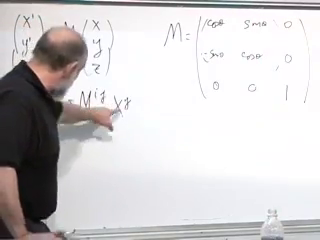
\includegraphics[width=0.82\textwidth]{lecture_05_figure_03.png}
\caption{الدوران المكاني مكتوبًا على هيئة معادلة مصفوفية وبترميز المؤشرات معًا.}
\lectureframe{01:00:40}
\end{figure}

\section{مصفوفات لورنتز وتركيب السرعات}

لحركة على طول \(x\)، يكون تحويل لورنتز في وحدات \(c=1\) هو
\begin{align}
x'&=\gamma_v(x-vt), & y'&=y,\nonumber\\
z'&=z, & t'&=\gamma_v(t-vx),
\end{align}
حيث
\begin{equation}
\gamma_v=\frac{1}{\sqrt{1-v^2}}.
\end{equation}
ومع ترتيب المركبات \((x,y,z,t)\)، يصبح ذلك
\begin{equation}
\begin{pmatrix}x'\\y'\\z'\\t'\end{pmatrix}
=
\begin{pmatrix}
\gamma_v&0&0&-\gamma_vv\\
0&1&0&0\\
0&0&1&0\\
-\gamma_vv&0&0&\gamma_v
\end{pmatrix}
\begin{pmatrix}x\\y\\z\\t\end{pmatrix}.
\label{eq:l5-lorentz-matrix}
\end{equation}

\begin{figure}[H]
\centering
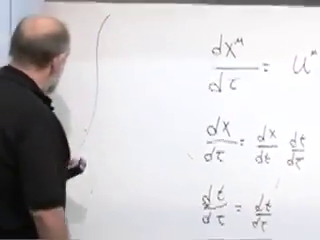
\includegraphics[width=0.82\textwidth]{lecture_05_figure_04.png}
\caption{مصفوفة لورنتز \(4\times4\). تختلط فقط المركبتان \(x\) و\(t\)؛ أما \(y\) و\(z\) فتبقيان دون تغير.}
\lectureframe{01:04:40}
\end{figure}

تجيب عملية ضرب المصفوفات الآن عن سؤال فيزيائي. افترض أن راصدًا يتحرك بسرعة \(v\) بالنسبة إلينا، وأن راصدًا ثالثًا يتحرك بسرعة \(u\) بالنسبة إلى ذلك الراصد، وجميع هذه الحركات على المحور نفسه. أما الحركيات النيوتونية فكانت ستعطي \(w=u+v\)، مما كان سيسمح بأن تتركب سرعتان كل منهما \(3c/4\) إلى \(3c/2\). لا بد أن تعطي النسبية قاعدة مختلفة.

الجزء الفعّال من تحويلة الدفع هو المصفوفة \(2\times2\)
\begin{equation}
B(v)=\gamma_v
\begin{pmatrix}1&-v\\-v&1\end{pmatrix}.
\end{equation}
ويعطي تركيب تحويلتي الدفع
\begin{align}
B(u)B(v)
&=\gamma_u\gamma_v
\begin{pmatrix}1&-u\\-u&1\end{pmatrix}
\begin{pmatrix}1&-v\\-v&1\end{pmatrix}\nonumber\\
&=\gamma_u\gamma_v
\begin{pmatrix}
1+uv&-(u+v)\\
-(u+v)&1+uv
\end{pmatrix}.
\label{eq:l5-composed-boost}
\end{align}
وتحدِّد نسبةُ مدخلٍ غير قطري إلى مدخلٍ قطري سرعةَ تحويلة الدفع الناتجة:
\begin{equation}
w=\frac{u+v}{1+uv}
\qquad(c=1).
\end{equation}
وبإعادة الأبعاد،
\begin{equation}
w=\frac{u+v}{1+uv/c^2}.
\label{eq:l5-velocity-addition}
\end{equation}

\begin{figure}[H]
\centering
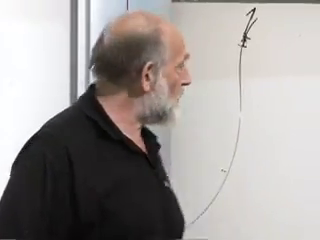
\includegraphics[width=0.82\textwidth]{lecture_05_figure_05.png}
\caption{مصفوفة تحويلة الدفع المركبة والسرعة
\(w=(u+v)/(1+uv)\) في الوحدات الطبيعية.}
\lectureframe{01:15:35}
\end{figure}

إذا كان كلٌّ من \(u\) و\(v\) قريبًا من \(c\)، فإن البسط يقترب من \(2c\)
بينما يقترب المقام من \(2\)، لذا تقترب \(w\) من \(c\)، لا من
\(2c\). وعلى نحو أعم، فإن المعادلة ~\eqref{eq:l5-velocity-addition} تحوِّل المدخلات دون الضوئية
إلى نتيجة دون ضوئية. وقد ضمَّنت عملية ضرب المصفوفات حدَّ السرعة
تلقائيًا.

\section{المتجهات الرباعية وفشل السرعة العادية}

المتجه الرباعي هو أي كائن تتحول مركباته الأربع تحت الدورانات
والدفعات اللورنتزية بالطريقة نفسها التي تتحول بها إحداثيات الزمكان. إذا كان \(V^\mu\)
متجهًا رباعيًا، فعند اعتماد اصطلاح الإشارة لدينا
\begin{equation}
V_\mu=(-V^1,-V^2,-V^3,V^0),
\end{equation}
ويكون معياره الثابت
\begin{equation}
V_\mu V^\mu=(V^0)^2-(V^1)^2-(V^2)^2-(V^3)^2.
\end{equation}
وبالنسبة إلى المتجهين الرباعيين \(V^\mu\) و\(W^\mu\)، فإن الانكماش
\begin{equation}
W_\mu V^\mu
=W^0V^0-W^1V^1-W^2V^2-W^3V^3
\end{equation}
هو أيضًا ثابت. تتغير المركبات من إطار مرجعي إلى آخر؛ أما الانكماش فلا يتغير.

للسرعة العادية ثلاث مركبات فقط،
\begin{equation}
\mathbf v=\left(\frac{dx}{dt},\frac{dy}{dt},\frac{dz}{dt}\right).
\end{equation}
وإلحاق \(dt/dt=1\) بها لا يجعلها متجهًا رباعيًا مفيدًا. فالمركبة الرابعة
ستكون تافهة، ولن يتحول الكائن الناتج خطيًا تحت
تحويلات لورنتز. يتغير الزمن الإحداثي \(t\) من إطار مرجعي إلى
آخر، لذلك فإن الاشتقاق بالنسبة إلى \(t\) يفسد قانون التحول المطلوب.

يوفّر الزمن الخاص الحل. على طول خط عالم نعرّف
\begin{equation}
u^\mu=\frac{dX^\mu}{d\tau}.
\label{eq:l5-four-velocity}
\end{equation}
التفاضل \(dX^\mu\) متجه رباعي و\(d\tau\) مقدار ثابت، لذا فإن
نسبتهما متجه رباعي. وتشير الصفة ``الخاص'' إلى الساعة الواردة في
المقام.

تربط قاعدة السلسلة هذا المقدار بالسرعة العادية:
\begin{equation}
\frac{dx}{d\tau}=\frac{dx}{dt}\frac{dt}{d\tau},
\end{equation}
وبالمثل بالنسبة إلى \(y\) و\(z\). من
المعادلة ~\eqref{eq:l5-proper-time}،
\begin{align}
\left(\frac{d\tau}{dt}\right)^2
&=1-\left(\frac{dx}{dt}\right)^2
    -\left(\frac{dy}{dt}\right)^2
    -\left(\frac{dz}{dt}\right)^2\nonumber\\
&=1-v^2
\qquad(c=1),
\end{align}
ومن ثم
\begin{equation}
\frac{dt}{d\tau}=\gamma_v=\frac{1}{\sqrt{1-v^2}}.
\end{equation}
والمركبات الأربع هي
\begin{equation}
u^i=\gamma_v v^i,
\qquad
u^0=\gamma_v
\qquad(c=1).
\label{eq:l5-four-velocity-components}
\end{equation}
عند السرعة الصغيرة، يكون \(u^i\simeq v^i\) و\(u^0\simeq1\). وأما قرب سرعة الضوء،
فإن \(\gamma_v\) يزداد بلا حد وتختلف السرعة الخاصة اختلافًا حادًا عن
السرعة العادية.

\begin{figure}[H]
\centering
\includegraphics[width=0.82\textwidth]{lecture_05_figure_06.png}
\caption{المركبات الأربع للسرعة الخاصة معبَّرًا عنها بدلالة السرعة العادية وعامل لورنتز.}
\lectureframe{01:34:40}
\end{figure}

بإرجاع الوحدات التقليدية واستخدام \(X^0=ct\) نحصل على الصورة القياسية
\begin{equation}
U^\mu=(\gamma_v\mathbf v,\gamma_v c)
\end{equation}
في الترتيب المستخدم هنا الذي تُقدَّم فيه المركبات المكانية أولًا. ومعياره الثابت هو
\begin{equation}
U_\mu U^\mu=c^2.
\end{equation}
وعليه، فلكل جسيم ذي كتلة سرعة رباعية لها المقدار الثابت نفسه، مع أن
سرعته المكانية تعتمد على الإطار المرجعي.

\section{المماس لخط العالم}

يوجد نظير إقليدي مألوف للمعادلة ~\eqref{eq:l5-four-velocity}.
فعلى طول منحنى في الفضاء الثلاثي الأبعاد العادي،
\begin{equation}
ds^2=dx^2+dy^2+dz^2.
\end{equation}
تشير الإزاحة التفاضلية \((dx,dy,dz)\) على امتداد المنحنى لكنها
ليست متجه وحدة. وبالقسمة على طول القوس نحصل على
\begin{equation}
\mathbf T=
\left(\frac{dx}{ds},\frac{dy}{ds},\frac{dz}{ds}\right),
\qquad
\mathbf T\cdot\mathbf T=1.
\end{equation}
والبناء النسبي هو الفكرة نفسها مع الزمن الخاص بدلًا من طول القوس
الإقليدي. والمتجه \(u^\mu=dX^\mu/d\tau\) مماس لخط
العالم.

\begin{figure}[H]
\centering
\includegraphics[width=0.82\textwidth]{lecture_05_figure_07.png}
\caption{بناء متجه المماس الإقليدي: اقسم الإزاحة التفاضلية
على عنصر طول القوس \(ds\). ويؤدي الزمن الخاص الدور المناظر
على طول خط عالم زمني.}
\lectureframe{01:39:30}
\end{figure}

\begin{classroomqa}
\audiencequestion{إذا كان \(c=1\)، فهل الزمن الخاص والمسافة الخاصة شيء واحد؟}
\lecturerresponse{إن وضع \(c=1\) يجعل الزمن والمسافة في الوحدات نفسها؛ لكنه
لا يمحو إشارات السالب في هندسة الزمكان. في النظير الإقليدي، تمثل \(s\)
المسافة العادية المقاسة على طول منحنى مكاني. وعلى طول خط عالم زمني، تمثل \(\tau\)
الزمن المنقضي الذي تقيسه ساعة. البناءان متشابهان، لكن الهندستين مختلفتان.}
\end{classroomqa}

وبأخذ المشتقة مرة أخرى نعرّف التسارع الخاص،
\begin{equation}
a^\mu=\frac{du^\mu}{d\tau}.
\end{equation}
وهذه هي الكمية التي يجب أن تحل محل \(d^2\mathbf x/dt^2\) عندما
يُصاغ قانون نيوتن الثاني صياغة نسبية. وبما أن \(u_\mu u^\mu\) ثابت،
\begin{equation}
\frac{d}{d\tau}(u_\mu u^\mu)=2u_\mu a^\mu=0,
\end{equation}
فإن التسارع الرباعي متعامد مينكوفسكيًا مع السرعة الرباعية.\editorialnote{وينتج
هذا التعامد مباشرة من المعيار الثابت، ويُدرج هنا بوصفه
النتيجة الرياضية التالية مباشرة للتعريف.}

\section{الزخم الرباعي والطاقة}

الزخم هو مثالنا الأخير لأنه ينحفظ في التصادمات والاضمحلالات.
وللجسيم كتلة ذاتية ثابتة \(m\)، تُسمّى كثيرًا كتلة سكونه. وهي
لا تتغير مع السرعة. والزخم النسبي هو تلك الكتلة الثابتة مضروبة في
السرعة الرباعية:
\begin{equation}
p^\mu=mu^\mu.
\label{eq:l5-four-momentum}
\end{equation}
وفي وحدات \(c=1\)،
\begin{equation}
p^i=\gamma_v m v^i,
\qquad
p^0=\gamma_v m.
\end{equation}
وعند السرعة الصغيرة يكون \(\gamma_v\simeq1\)، لذا تختزل المركبات المكانية إلى
الزخم النيوتني \(m\mathbf v\). وعند السرعة العالية تنمو أسرع
من \(m\mathbf v\).

المركبة الزمنية هي الطاقة. ومع الوحدات التقليدية و\(X^0=ct\)،
\begin{equation}
P^\mu=(\mathbf p,E/c)
=(\gamma_v m\mathbf v,\gamma_v mc),
\end{equation}
ومن ثم
\begin{equation}
E=\gamma_v mc^2
=mc^2\left(1-\frac{v^2}{c^2}\right)^{-1/2}.
\label{eq:l5-relativistic-energy}
\end{equation}

لاستعادة الميكانيكا العادية، لنضع
\(\epsilon=v^2/c^2\ll1\). ويعطي توسع ذي الحدين
\begin{equation}
(1-\epsilon)^p=1-p\epsilon+O(\epsilon^2).
\end{equation}
وبأخذ \(p=-1/2\)،
\begin{align}
E
&=mc^2\left(1-\frac{v^2}{c^2}\right)^{-1/2}\nonumber\\
&=mc^2\left[1+\frac12\frac{v^2}{c^2}
  +O\!\left(\frac{v^4}{c^4}\right)\right]\nonumber\\
&=mc^2+\frac12mv^2+O\!\left(\frac{mv^4}{c^2}\right).
\label{eq:l5-energy-expansion}
\end{align}

\begin{figure}[H]
\centering
\includegraphics[width=0.82\textwidth]{lecture_05_figure_08.png}
\caption{توسع الطاقة النسبية عند السرعات الصغيرة، كاشفًا عن طاقة السكون والطاقة الحركية النيوتنية.}
\lectureframe{01:51:30}
\end{figure}

الحد الأول، \(mc^2\)، موجود حتى في السكون. ففي مسألة نيوتنية تضم
مجموعة ثابتة من الجسيمات وكتلًا لا تتغير، يضيف ذلك الحد
القيمة الثابتة نفسها قبل الحركة وبعدها، لذلك لا يؤثر في الحسابات
المألوفة إلا \(\tfrac12mv^2\). وتكشف النسبية أن ذلك الثابت المستبعَد
كان طاقة فيزيائية منذ البداية.

ولذلك فليست الطاقة والزخم قانوني انحفاظ منفصلين لا صلة بينهما. بل هما
المركبات الأربع لمتجه واحد محفوظ. وتمزجهما دفعة لورنتزية: فما
يسميه راصد ما طاقةً يسهم جزئيًا في زخم راصد آخر،
والعكس صحيح. ومع ذلك، ففي نظام معزول يكون الزخم الرباعي الكلي
هو نفسه قبل كل تصادم أو اضمحلال وبعده في كل إطار عطالي.

هذه هي عتبة الميكانيكا النسبية. والمهمتان التاليتان هما التعبير عن
القوة بدلالة التسارع الخاص، وفهم معادلات الموجة النسبية،
وخاصة المعادلات التي تحكم الكهرومغناطيسية والضوء.

\chapter{القوانين الثابتة، والمتجهات الرباعية، وموتر المجال}

سنبدأ بقانون كان يمكن للطبيعة أن تمتثل له، لكنها لا تفعل. وسيكشف لنا إخفاقه كيف ينبغي أن يُكتب القانون الفيزيائي. والاختبار نفسه يقود أولًا من مركبات الإحداثيات إلى المتجهات العادية، ثم من المتجهات العادية إلى المتجهات الرباعية، وأخيرًا من المتجهات الرباعية إلى الموترات. وبحلول النهاية، لن يعود المجالان الكهربائي والمغناطيسي جسمين منفصلين: بل سيشغلان معًا الخانات الست المستقلة لموتر واحد متضاد التناظر.

ما لم يُذكر خلاف ذلك، نستخدم وحدات يكون فيها \(c=1\)، ونرتب مركبات الزمكان على النحو \((1,2,3,0)=(x,y,z,t)\)، ونستخدم اصطلاح إشارة المترية \((-,-,-,+)\).

\section{قانون ممكن ذو تناظر خاطئ}

ثبّت محورًا \(x\) ومحورًا \(y\) تثبيتًا دائمًا في الفضاء. ولنفرض الآن أن جسيمين يتفاعلان كلما تساوت إحداثياتهما \(x\). قد يعكس التفاعل حركتهما أو يرسلهما مبتعدين في اتجاهات جديدة؛ وديناميكا هذا التفاعل التفصيلية لا تهم. وشرط البدء المقترح هو ببساطة \begin{equation}
  x_1-x_2=0,
\end{equation} حيث تشير الرموز السفلية إلى الجسيمات لا إلى مركبات الإحداثيات. ولا يوجد في هذه القاعدة أي تناقض رياضي. والسؤال هو: ما الذي يجعلها غير معقولة فيزيائيًا؟

\begin{classroomqa} \audiencequestion{هل تنتهك هذه القاعدة تجانس الفضاء؟} \lecturerresponse{لا. إن نقل المبدأ يغيّر الإحداثيين بالمقدار نفسه ويترك \(x_1-x_2\) دون تغيير. ولا تحدد هذه القاعدة أي موضع مفضّل. أما عيبها فهو تماثل الخواص في جميع الاتجاهات: فهي تميّز اتجاهًا مفضّلًا واحدًا.} \end{classroomqa}

أدِر المحاور بزاوية \(90^\circ\). فالجهة القديمة \(x\) تُسمّى الآن \(y\)، ولذلك ستوصَف الأحداث الفيزيائية نفسها بتساوي الإحداثيين \(y\). وعند زاوية عامة سيدخل في الشرط تركيب خطي من \(x\) و\(y\). ولذلك تعتمد صيغة القانون على الكيفية التي وُجّهت بها السبورة. فهو ثابت تحت الإزاحة، لكنه غير ثابت تحت الدوران.

نعطي القوانين الفيزيائية عادة أبسط صورها في إحداثيات متعامدة. ويمكن استعمال إحداثيات أكثر عمومية، لكن المترية والصيغ تصبحان عندئذ أقل بساطة. وضمن فئة الأطر الديكارتية المتعامدة، لا ينبغي تمييز أي توجّه.

والإصلاح فوري. ففي بُعدين نطلب تساوي الإحداثيين كليهما؛ وفي ثلاثة أبعاد نطلب تساوي الإحداثيات الثلاث كلها: \begin{equation}
  x_1=x_2,
  \qquad y_1=y_2,
  \qquad z_1=z_2.
\end{equation} وعندئذ لا يمكن للجسيمين أن يتفاعلا إلا عندما يبلغان النقطة نفسها، حتى لو اقتربا منها على امتداد خطين مختلفين.

\begin{classroomqa} \audiencequestion{وهل يجب أن تتساوى أيضًا إحداثيات \(z\) والأزمنة؟} \lecturerresponse{في الفضاء الثلاثي الأبعاد يجب أن تتساوى أيضًا إحداثيات \(z\). ويُغفَل الزمن في الوقت الراهن؛ وسيُعاد إدخاله ما إن يكتمل البرهان المكاني.} \end{classroomqa}

لتكن \(\boldsymbol r_a\) موضع الجسيم \(a\). تصبح شروط المركبات الثلاثة معادلة متجهية واحدة، \begin{equation}
  \boldsymbol r_1-\boldsymbol r_2=\boldsymbol 0.
\end{equation} قد تنعدم مركبة في إطار مُدار ما، ولا تنعدم في إطار مُدار آخر. أما المتجه كله فالأمر مختلف: فإذا كانت كل مركبة فيه صفرًا في إطار ما، كانت كل مركبة فيه صفرًا في كل إطار مُدار. وكذلك إذا كان متجهان متساويين في إطار ما، فإنهما يظلان متساويين بعد تحويلهما معًا.

\begin{figure}[H] \centering
\includegraphics[width=0.78\textwidth]{lecture_06_figure_01.png} \caption{تساوي الإحداثيات الثلاثة الذي يجعل التصادم يعني التطابق المكاني بدلًا من التطابق على طول محور مفضّل واحد.} \lectureframe{00:09:00} \end{figure}

ولهذا تكون المعادلات المتجهية مفيدة. فمركباتها تتغير، لكن الكمية نفسها تتحول على نحو متسق. ويمكن لقانون يُكتب للكمية الكاملة أن يحتفظ بصيغته عندما تُدار الإحداثيات.

\section{التطابق في الزمكان}

استبدل الآن المحور المكاني الرأسي بالزمن. فقد تقول قاعدة نيوتونية إن تغيرين في الحركة لا يحدثان إلا عند أزمنة متساوية. ففي الميكانيكا النيوتونية يكون التزامن مشتركًا بين جميع المراقبين العطاليين، ولذلك تكون مثل هذه القاعدة ممكنة. أما في النسبية الخاصة فإنها تنتقي إطارًا مفضّلًا. فالأحداث المتزامنة في إطار ما لا يلزم أن تكون متزامنة في إطار آخر.

وليس اشتراط تساوي الإحداثيات المكانية وحدها أفضل حالًا. فقد تكون لإزاحة زمكانية مركبات مكانية منعدمة ومركبة زمنية غير منعدمة، \begin{equation}
  \Delta X^\mu=(0,0,0,\Delta t),
\end{equation} ويخلط التعزيز \(\Delta t\) بمركبة مكانية. والعبارة المحلية الثابتة هي أن التغيرين في الحركة يقعان عند الحدث نفسه. لذلك يتطلب تصادم بسيط \begin{equation}
  X_1^\mu=X_2^\mu,
  \qquad\text{or}\qquad
  X_1^\mu-X_2^\mu=0.
\end{equation} تتساوى الإحداثيات الأربع كلها: فالجسيمان يشغلان المكان نفسه في الزمن نفسه.

يعطي مثال التصادم قاعدة عامة لكتابة الفيزياء. يمكننا أن نضع كل شيء في طرف واحد ونجعل متجهًا رباعيًا كاملًا مساويًا للصفر، أو نجعل متجهًا رباعيًا كاملًا مساويًا لمتجه رباعي كامل آخر. أما مساواة أجزاء منفصلة من متجه رباعي، فلا تعطي في حد ذاتها عبارة ثابتة لورنتزيًا.

\section{التعزيزات، والدورانات، وترميز المصفوفات}

المتجه الرباعي هو كمية تتحول كما تتحول إزاحة زمكانية. ولكي يصبح هذا التعريف مفيدًا، تذكّر أولًا تحولات الإحداثيات نفسها. فبالنسبة إلى تعزيز بسرعة \(v\) في اتجاه \(x\)، \begin{align}
  x'&=\gamma(x-vt), & y'&=y, & z'&=z,
  & t'&=\gamma(t-vx),                                      \label{eq:l6-boost}
\end{align} حيث \begin{equation}
  \gamma(v)=\frac{1}{\sqrt{1-v^2}}.
\end{equation}

\begin{classroomqa} \audiencequestion{هل جُعلت سرعة الضوء مساوية للواحد في هذه الصيغ؟} \lecturerresponse{نعم. عند إعادة الوحدات، خذ \(X^0=ct\)، واستبدل \(1-v^2\) بـ \(1-v^2/c^2\)، وأعِد العوامل المناظرة من \(c\) في الحدود المختلطة مكان--زمان.} \end{classroomqa}

إن دورانًا حول المحور \(z\) يخلط \(x\) و\(y\)، ويترك \(z\) و\(t\) على حالهما: \begin{equation}
\begin{pmatrix}
  x'\\ y'\\ z'\\ t'
\end{pmatrix}
=
\begin{pmatrix}
  \cos\theta & \sin\theta & 0 & 0\\
  -\sin\theta & \cos\theta & 0 & 0\\
  0 & 0 & 1 & 0\\
  0 & 0 & 0 & 1
\end{pmatrix}
\begin{pmatrix}
  x\\ y\\ z\\ t
\end{pmatrix}.
\end{equation} ويجدر إظهار الأصفار: فهي تُبيّن صراحةً أي المركبات لا تدخل في إحداثي مُحوَّل معيّن. وبالترتيب نفسه، يكون التعزيز في المعادلة~\eqref{eq:l6-boost} هو \begin{equation}
\begin{pmatrix}
  x'\\ y'\\ z'\\ t'
\end{pmatrix}
=
\begin{pmatrix}
  \gamma & 0 & 0 & -\gamma v\\
  0 & 1 & 0 & 0\\
  0 & 0 & 1 & 0\\
  -\gamma v & 0 & 0 & \gamma
\end{pmatrix}
\begin{pmatrix}
  x\\ y\\ z\\ t
\end{pmatrix}.
\end{equation}

يمكن تركيب الدورانات والتعزيزات بضرب المصفوفات. ولإجراء تعزيز في اتجاه غير مصطفٍّ مع المحور الأصلي \(x\)، يمكن إدارة ذلك الاتجاه إلى المحور \(x\)، ثم تطبيق التعزيز، ثم إدارة المحاور حسب الحاجة. وتولّد جداءات هذه المصفوفات الأولية تحولات لورنتز أكثر عمومية.

\begin{classroomqa} \audiencequestion{هل يهمّ ما إذا أُجري الدوران أولًا ثم التعزيز، أم التعزيز أولًا ثم الدوران؟} \lecturerresponse{نعم. فبعد العملية الأولى تكون المحاور التي تؤثر فيها العملية الثانية قد تغيّرت. وليس لازمًا أن يتطابق جداءا المصفوفتين، ولذلك يهم ترتيب العمليات.} \end{classroomqa}

يمكن كتابة جميع هذه التحولات الخطية دفعةً واحدة على الصورة \begin{equation}
  X'^{\mu}=\Lambda^{\mu}{}_{\nu}X^{\nu}.                  \label{eq:l6-vector-transform}
\end{equation} ويُجمع على المؤشر المكرر \(\nu\) عبر \(1,2,3,0\). وهذا ليس إلا الجمع المعتاد صفًّا بعمود في ضرب المصفوفات، معبَّرًا عنه بترميز المؤشرات.

\begin{figure}[H] \centering
\includegraphics[width=0.78\textwidth]{lecture_06_figure_02.png} \caption{تحويل لورنتز ذي المؤشرات في الأعلى، وبداية صيغته على هيئة متجه عمودي.} \lectureframe{00:31:55} \end{figure}

والمعادلة~\eqref{eq:l6-vector-transform} هي أيضًا تعريف المتجه الرباعي العام المضاد للتغاير. فإذا كان \(A^\mu\) متجهًا من هذا النوع، فإن \begin{equation}
  A'^{\mu}=\Lambda^{\mu}{}_{\nu}A^{\nu}.
\end{equation} ولا يلزم أن تمثل مركباته الأربع موضعًا. وما يجعل هذه الكمية متجهًا رباعيًا هو قانون تحولها.

\section{الكميات القياسية، والمترية، والجداءات الثابتة}

قبل استخدام مزيد من المتجهات الرباعية، من المفيد أن نعود خطوة إلى الوراء نحو المفهوم الأبسط للكمية القياسية. فدرجة الحرارة عند نقطة محددة كمية قياسية تحت الدورانات المكانية، وكذلك المسافة بين نقطتين محددتين. وكل منهما عدد واحد مستقل عن توجّه المحاور. بل يمكن حتى إطلاق الادعاء العددي السخيف عمدًا بأن مسافةً مقاسة بالسنتيمترات تساوي درجة حرارة الغرفة المقاسة بدرجات فهرنهايت. وليس لهذا الادعاء عمق فيزيائي، لكن لأن كلا الطرفين كميتان قياسيتان دورانيًا، فإن صدقه أو كذبه لا يعتمد على كيفية إدارة المحاور.

ومركبات المتجه ليست كميات قياسية. ولذلك نحتاج إلى طريقة منهجية لتركيبها في كميات قياسية. اكتب متجهًا رباعيًا عامًا مضادّ التغاير على الصورة \begin{equation}
  A^\mu=(A^1,A^2,A^3,A^0).
\end{equation} وتصف المركبات المتغايرة الكائن الهندسي نفسه بمؤشر سفلي. ومع اصطلاح الإشارة الذي نتبعه، تُستحصل هذه المركبات باستخدام مترية مينكوفسكي، \begin{equation}
  A_\mu=\eta_{\mu\nu}A^\nu,
  \qquad
  \eta_{\mu\nu}=
  \begin{pmatrix}
    -1&0&0&0\\
    0&-1&0&0\\
    0&0&-1&0\\
    0&0&0&1
  \end{pmatrix},                                          \label{eq:l6-metric}
\end{equation} بحيث يكون \begin{equation}
  A_\mu=(-A^1,-A^2,-A^3,A^0).
\end{equation}

\begin{classroomqa} \audiencequestion{هل يوجد عدم اتساق بين مؤشرين وإشارتين على السبورة؟} \lecturerresponse{نعم. فالمركبة المكانية في العمود المعروض تحتاج إلى إشارة السالب المناظرة، والمركبات الواقعة إلى يمين معادلة إنزال المؤشر تحمل مؤشرات علوية قبل الضرب في \(\eta_{\mu\nu}\). ووسم الزمن هو \(0\) لا \(4\).} \end{classroomqa}

\begin{figure}[H] \centering
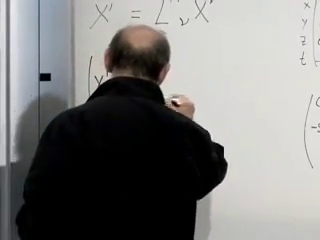
\includegraphics[width=0.8\textwidth]{lecture_06_figure_03.png} \caption{المركبات المضادة للتغاير والمتغايرة، ومصفوفة المترية، وبداية التقلص الثابت.} \lectureframe{00:45:00} \end{figure}

إنزال المؤشر ليس مجرد زخرفة. فهو يجمع الإشارات اللازمة للمعيار الثابت تحت لورنتز: \begin{align}
  A_\mu A^\mu
  &=-(A^1)^2-(A^2)^2-(A^3)^2+(A^0)^2,                    \label{eq:l6-norm}\\
  X_\mu X^\mu
  &=t^2-x^2-y^2-z^2.
\end{align} والتعبير الثاني هو الفاصل الزمكاني الثابت من نقطة الأصل. ولأن \(A^\mu\) يتحول بالطريقة نفسها التي يتحول بها \(X^\mu\)، فإن تقلصه يتمتع بالثبات نفسه.

ويعلّمنا هذا الترميز أيضًا قاعدة مفيدة في ضبط المؤشرات. فمؤشر الجمع المكرر يظهر مرة في الموضع العلوي ومرة في الموضع السفلي. فمثلًا، \begin{equation}
  A_\mu A^\mu
  =\eta_{\mu\nu}A^\mu A^\nu.
\end{equation} ويمكن تغيير أسماء مؤشرات الجمع، أو المؤشرات الصورية، من غير أن تتغير الكمية.

\begin{classroomqa}
\audiencequestion{هل ينبغي اعتبار أحد هذين المتجهين صفًا والآخر عمودًا، وهل يهم ترتيبهما؟}
\lecturerresponse{في هذا الحساب الحالي، اعتبر الكميات ذات الفهارس مركباتٍ ودَعِ المتريّة تُجري الانكماش؛ فلا حاجة إلى تحويل النقاش إلى جبر مؤثرات من نوع صفّ مقابل عمود. فهذه أعداد عادية، ولذلك لا يهم ترتيبها. أما المؤثرات غير المتبادلة فتتطلب مزيدًا من العناية، لكن هذا ليس موضوعنا هنا.}
\end{classroomqa}

ويعطي البناء نفسه جداءً داخليًا بين متجهين رباعيين مختلفين،
\begin{equation}
  A\mathbin{\cdot}B=A_\mu B^\mu=A^\mu B_\mu.
\end{equation}
وتتبع ثباتيته من دون كتابة مصفوفة لورنتز صريحة. وبما أن \(A+B\) و\(A-B\) متجهان رباعيان، فإن مربع معيار كلٍّ منهما ثابت:
\begin{align}
  (A+B)^2&=A^2+B^2+2A\mathbin{\cdot}B,\\
  (A-B)^2&=A^2+B^2-2A\mathbin{\cdot}B.
\end{align}
وبالطرح نحصل على
\begin{equation}
  (A+B)^2-(A-B)^2=4A\mathbin{\cdot}B,                    \label{eq:l6-polarization}
\end{equation}
ومن ثم فإن \(A\mathbin{\cdot}B\) ثابت أيضًا. وينتج العامل أربعة مباشرةً من التوسيع.\editorialnote{تُقدِّم الحجة المعروضة على اللوح هوية الاستقطاب هذه؛ وكتابة العامل صراحةً تجعل الإلغاء المذكور شفهيًا غير ملتبس.}

\begin{figure}[H]
\centering
\includegraphics[width=0.8\textwidth]{lecture_06_figure_04.png}
\caption{المربعان الثابتان المستخدمان لعزل الجداء الداخلي لمتجهين رباعيين مختلفين.}
\lectureframe{00:52:20}
\end{figure}

الكميات الثابتة مكوّنات طبيعية في القوانين الفيزيائية: فهي، بخلاف مركبة منفردة، تحمل القيمة نفسها من إطار مرجعي إلى آخر.

\section{السرعة الخاصة والزخم الرباعي}

لننظر إلى حدثين متجاورين على خط عالم جسيم. فإن الفاصل بينهما هو المتجه الرباعي التفاضلي المتناهي في الصغر
\begin{equation}
  dX^\mu=(dx,dy,dz,dt).
\end{equation}
وبالنسبة إلى خط عالم زمني، يُعرَّف الزمن الخاص بـ
\begin{equation}
  d\tau^2=dX_\mu dX^\mu
  =dt^2-dx^2-dy^2-dz^2.                                  \label{eq:l6-proper-time}
\end{equation}
والسرعة الرباعية الخاصة هي
\begin{equation}
  U^\mu=\frac{dX^\mu}{d\tau}.                            \label{eq:l6-four-velocity}
\end{equation}
وهي تقيس معدل تغيّر موضع الزمكان بالنسبة إلى الزمن الخاص للجسيم نفسه، لا بالنسبة إلى الزمن الإحداثي لإطار مرجعي مختار.

مع أن \(U^\mu\) له أربع مركبات، فإن ثلاثًا فقط منها مستقلة. وبقسمة المعادلة ~\eqref{eq:l6-proper-time} على \(d\tau^2\) نحصل على
\begin{equation}
  U_\mu U^\mu=1.
\end{equation}
ومن ثم فإن السرعة الرباعية متجه زمني معياره واحد. ويحدِّد اختيار الاتجاه نحو المستقبل إشارة مركبته الزمنية.

\begin{classroomqa}
\audiencequestion{عند سرعات أصغر بكثير من \(c\)، هل تؤول السرعة الرباعية إلى السرعة العادية؟}
\lecturerresponse{تقترب مركباتها المكانية الثلاث من السرعة العادية، بينما تقترب مركبتها الزمنية من الواحد في وحدات \(c=1\). وتنتج هذه العلاقة من تطبيق قاعدة السلسلة وحساب \(dt/d\tau\).}
\end{classroomqa}

أما لكل مركبة مكانية، فلدينا
\begin{equation}
  U^i=\frac{dx^i}{d\tau}
     =\frac{dx^i}{dt}\frac{dt}{d\tau}
     =v^i\frac{dt}{d\tau}.
\end{equation}
وبقسمة المعادلة ~\eqref{eq:l6-proper-time} على \(dt^2\) نحصل على:
\begin{equation}
  \left(\frac{d\tau}{dt}\right)^2
  =1-v_x^2-v_y^2-v_z^2
  =1-\boldsymbol v^2.
\end{equation}
ومن ثم
\begin{equation}
  \frac{dt}{d\tau}=\frac{1}{\sqrt{1-\boldsymbol v^2}}
  =\gamma(\lvert\boldsymbol v\rvert),
\end{equation}
و
\begin{equation}
  U^\mu=(\gamma v_x,\gamma v_y,\gamma v_z,\gamma).
                                                                  \label{eq:l6-u-components}
\end{equation}

\begin{figure}[H]
\centering
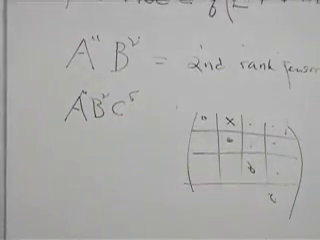
\includegraphics[width=0.8\textwidth]{lecture_06_figure_05.png}
\caption{حساب الزمن الخاص الذي ينتج \(dt/d\tau=\gamma\) ويربط السرعة الخاصة بالسرعة العادية.}
\lectureframe{01:02:00}
\end{figure}

\begin{classroomqa}
\audiencequestion{هل تعني \(dx^2/dt^2\) مشتقةً ثانية، وهل ينبغي أن ينتج عن تربيع متجه حدود مختلطة؟}
\lecturerresponse{هنا تعني \((dx/dt)^2\)، أي مربع مشتقة أولى. وعلاوة على ذلك، تعني \(\boldsymbol v^2\) الجداء النقطي الإقليدي \(v_x^2+v_y^2+v_z^2\)، لا مربع المجموع الصوري \(v_x+v_y+v_z\)؛ ولا توجد حدود مختلطة.}
\end{classroomqa}

\begin{classroomqa}
\audiencequestion{هل تمثل \(v\) في \(\gamma(v)\) السرعة النسبية لإطارين إحداثيين أم سرعة الجسيم؟}
\lecturerresponse{هنا هي سرعة الجسيم في الإطار المختار. ويمكن تقييم الدالة \(\gamma(v)=1/\sqrt{1-v^2}\) عند أي سرعة: ففي تحويل دفعي تُقيَّم عند السرعة النسبية بين الإطارين؛ وفي السرعة الرباعية تُقيَّم عند سرعة الجسيم.}
\end{classroomqa}

عندما يكون \(v\ll1\)، يكون \(\gamma\simeq1\)، لذا تقترب المركبات المكانية لـ \(U^\mu\) من \(\boldsymbol v\) وتقترب \(U^0\) من الواحد. ومع اقتراب السرعة العادية من سرعة الضوء، يزداد \(\gamma\) وجميع المركبات غير الصفرية للسرعة الرباعية بلا حد.

\begin{classroomqa}
\audiencequestion{ألا ينبغي أن تكون لـ \(U^0\) وحدات سرعة بدلًا من أن تكون قريبة من العدد واحد؟}
\lecturerresponse{اختفت الوحدات عندما جُعل \(c\) مساويًا للواحد. ومع \(X^0=ct\)، يكون لدينا
\(U^\mu=(\gamma\boldsymbol v,\gamma c)\)، لذا تقترب المركبة الزمنية من \(c\) ويصبح \(U_\mu U^\mu=c^2\).}
\end{classroomqa}

لجسيم كتلته السكونية \(m\)، نعرّف الزخم الرباعي بـ
\begin{equation}
  P^\mu=mU^\mu.
\end{equation}
في الوحدات الطبيعية،
\begin{equation}
  P^\mu=(\gamma m\boldsymbol v,\gamma m).
\end{equation}
تقترب المركبات الثلاث الأولى من الزخم النيوتني \(m\boldsymbol v\) عند السرعات المنخفضة. وبإعادة الوحدات نحصل على
\begin{equation}
  P^\mu=(\gamma m\boldsymbol v,E/c),
  \qquad E=\gamma mc^2,
\end{equation}
ومن ثم
\begin{equation}
  E=mc^2+\frac{1}{2}m\boldsymbol v^2+O(mv^4/c^2).
\end{equation}
المركبة الزمنية هي الطاقة بوحدات \(c=1\)، أو الطاقة مقسومة على \(c\) عندما تُعطى جميع المركبات الأربع وحدات الزخم.

\begin{classroomqa}
\audiencequestion{هل تكون \(\boldsymbol v\) العادية، مع إلحاق مركبة رابعة بها، متجهًا رباعيًا بحد ذاتها؟}
\lecturerresponse{لا. السرعة الثلاثية العادية لا تتحول كمتجه رباعي. العامل \(\gamma\) وتعريف الزمن الخاص أساسيان؛ فالمتجه الرباعي هو \(U^\mu\)، وليس \(\boldsymbol v\).}
\end{classroomqa}

\section{لماذا يجب أن يختلط المجالان الكهربائي والمغناطيسي}

نأخذ الآن ما سُمّي استراحة قصيرة من النسبية. لنبدأ بمعادلة الحركة ما قبل أينشتاين ونسأل كيف يجب إعادة تنظيمها قبل أن تصبح صالحة في كل إطار قصوري. التسارع العادي هو المشتقة الزمنية للسرعة العادية. ونظيره رباعي الأبعاد هو بطبيعة الحال
\begin{equation}
  A^\mu=\frac{dU^\mu}{d\tau}.
\end{equation}
عند السرعات المنخفضة، تقترب مركباته المكانية من التسارع العادي. سنؤجل المعادلة النسبية الكاملة؛ ولنعاين أولًا قانون القوة القديم.

بالنسبة إلى شحنة \(q\) في مجالين كهربائي ومغناطيسي،
\begin{equation}
  \boldsymbol F=m\boldsymbol a
  =q\left(\boldsymbol E+\boldsymbol v\times\boldsymbol B\right).
                                                                  \label{eq:l6-lorentz-force}
\end{equation}
الحد الكهربائي مستقل عن سرعة الجسيم، في حين أن الحد المغناطيسي ليس كذلك.

\begin{figure}[H]
\centering
\includegraphics[width=0.8\textwidth]{lecture_06_figure_06.png}
\caption{الصيغة ما قبل النسبية لقانون قوة لورنتز التي تحفّز على الجمع بين \(\boldsymbol E\) و\(\boldsymbol B\).}
\lectureframe{01:18:20}
\end{figure}

افترض أن راصدًا لا يرى مجالًا كهربائيًا، لكنه يرى مجالًا مغناطيسيًا وشحنة متحركة. تتعرض الشحنة لقوة مغناطيسية. غير أنه في إطار السكون اللحظي للشحنة، \(\boldsymbol v=0\)، ولذلك ينعدم الحد المغناطيسي في المعادلة~\eqref{eq:l6-lorentz-force}. ولم يصبح خط العالم الفيزيائي قصوريًا لمجرد أن الإحداثيات تغيّرت؛ لذا لا بد أن تشتمل القوة في الإطار الجديد على مساهمة كهربائية. وبصياغة أدق، لا يمكن تحويل تسارع رباعي غير صفري إلى الصفر بمجرد تغيير الأطر القصورية، مع أن التسارع الثلاثي ومركباته يتحولان بالفعل. \editorialnote{تمثل عبارة التسارع الرباعي هذه الصيغة اللامتغيرة للحجة المطروحة في قاعة الدرس، وتتجنب التعامل مع التسارع الثلاثي العادي نفسه على أنه لا يتغير بتغير الإطار.}

وعليه، يجب أن يتحول المجالان الكهربائي والمغناطيسي أحدهما إلى الآخر. ولهما معًا ست مركبات، لذلك فهما ليسا كمية قياسية واحدة ولا متجهًا رباعيًّا واحدًا. نحتاج إلى كائن جديد ذي قانون تحول.

\section{الموترات: تحول واحد لكل فهرس}

يجوز أن تُسمى الكمية القياسية موترًا من الرتبة صفر؛ فهي لا تملك فهارس. والمتجه الرباعي موتر من الرتبة الأولى؛ وله فهرس واحد له أربع قيم ممكنة. وأبسط مثال من الرتبة الثانية هو الجداء
\begin{equation}
  A^\mu B^\nu.
\end{equation}
ولكل فهرس أربع قيم، لذا يملك هذا الكائن \(4^2=16\) مركبة، ويمكن عرضها في هيئة مصفوفة \(4\times4\). أما جداء ثلاثة متجهات،
\begin{equation}
  A^\mu B^\nu C^\sigma,
\end{equation}
فله \(4^3=64\) مركبة، وهو موتر من الرتبة الثالثة. وتستمر الرتب الأعلى على هذا النمط. والاسم أقل أهمية من القاعدة التي تعرّف هذا الكائن.

إذا كان
\begin{equation}
  A'^{\mu}=\Lambda^\mu{}_{\nu}A^\nu,
  \qquad
  B'^{\sigma}=\Lambda^\sigma{}_{\tau}B^\tau,
\end{equation}
فإن جداءهما يتحول على النحو
\begin{equation}
  A'^{\mu}B'^{\sigma}
  =\Lambda^\mu{}_{\nu}\Lambda^\sigma{}_{\tau}
   A^\nu B^\tau.
\end{equation}
وهذا يعطينا القانون التعريفي لموتر مضادّ التغاير من الرتبة الثانية:
\begin{equation}
  T'^{\mu\sigma}
  =\Lambda^\mu{}_{\nu}\Lambda^\sigma{}_{\tau}T^{\nu\tau}.
                                                                  \label{eq:l6-tensor-transform}
\end{equation}
توجد مصفوفة لورنتز واحدة لكل فهرس. ويُجمَع على \(\nu\) و\(\tau\) المكررين؛ أما \(\mu\) و\(\sigma\) الحرّان فيحددان المركبة الجاري حسابها في الإطار المشار إليه بشرطة.

\begin{figure}[H]
\centering
\includegraphics[width=0.82\textwidth]{lecture_06_figure_07.png}
\caption{تحول متجهين، وقانون التحول الناتج ذي المصفوفتين لموتر من الرتبة الثانية.}
\lectureframe{01:27:15}
\end{figure}

لا يشترط أن يكون الموتر جداءً واحدًا لمتجهات. فكل من \(A^\mu B^\nu\) و\(A^\nu B^\mu\) يخضع لقانون تحول الموتر، وكذلك مجموعهما وأي مجموع من قبيل
\begin{equation}
  A^\mu B^\nu+C^\mu D^\nu.
\end{equation}
فقانون التحول، لا تحليل معيّن إلى عوامل، هو التعريف. ويكتسب موتر من الرتبة الثالثة مصفوفة لورنتز ثالثة، وهكذا.

\section{الموترات المتناظرة والمضادة للتناظر}

ستكون فئتان من موترات الرتبة الثانية مفيدتين على نحو خاص. فالموتر المتناظر يحقق
\begin{equation}
  T^{\mu\nu}=T^{\nu\mu},
\end{equation}
بحيث تتطابق العناصر المنعكسة عبر القطر. وتحدد عناصره الأربعة الواقعة على القطر وستة عناصر على أحد جانبي القطر بقية العناصر، فنحصل على
\begin{equation}
  4+6=10
\end{equation}
مركبات مستقلة.

أما الموتر المضاد للتناظر فيحقق
\begin{equation}
  T^{\mu\nu}=-T^{\nu\mu}.                                \label{eq:l6-antisymmetry}
\end{equation}
وبوضع \(\mu=\nu\) في المعادلة~\eqref{eq:l6-antisymmetry} نحصل على
\(T^{\mu\mu}=-T^{\mu\mu}\)، ولذلك ينعدم كل عنصر قطري. وتحدد العناصر الستة في أحد النصفين المثلثيين العناصر الستة الأخرى بتغير في الإشارة. ولذلك توجد بالضبط ست مركبات مستقلة.

\begin{figure}[H]
\centering
\includegraphics[width=0.82\textwidth]{lecture_06_figure_08.png}
\caption{مصفوفة \(4\times4\) مضادّة التناظر مكتملة: أصفار على القطر
وعلامات متعاكسة على جانبيه.}
\lectureframe{01:34:25}
\end{figure}

هذا العدد هو المفتاح. فالمركبات الكهربائية الثلاث والمركبات المغناطيسية الثلاث يمكن أن تنتظم في موتر واحد مضادّ التناظر من الرتبة الثانية.

\section{موتر المجال الكهرومغناطيسي}

لتكن وسوم الزمكان عبر الصفوف والأعمدة بالترتيب
\((1,2,3,0)=(x,y,z,t)\). والترتيب المكتوب على اللوح هو
\begin{equation}
  F_{\mu\nu}=
  \begin{pmatrix}
    0    & -B_3 & B_2  & E_1\\
    B_3  & 0    & -B_1 & E_2\\
    -B_2 & B_1  & 0    & E_3\\
    -E_1 & -E_2 & -E_3 & 0
  \end{pmatrix}.                                         \label{eq:l6-field-tensor}
\end{equation}
تحتوي الخانات المكانية البحتة على المجال المغناطيسي؛ أما الخانات التي تحمل مؤشرًا مكانيًا وآخر زمنيًا فتحتوي على المجال الكهربائي. ويعطي ضدّ التناظر عناصر المثلث السفلي متى عُرفت عناصر المثلث العلوي.

\begin{classroomqa}
\audiencequestion{هل جميع المدخلات المغناطيسية سالبة، وهل تقابل الوسوم
\(x,y,z\)؟}
\lecturerresponse{تتناوب الإشارات في المثلث المكاني العلوي كما هو مبيّن:
\(-B_3,+B_2,-B_1\). والوسوم \(1,2,3\) تقابل \(x,y,z\)، بينما
\(0\) يوسم الزمن. والانعكاس عبر القطر يعكس كل إشارة.}
\end{classroomqa}

\begin{figure}[H]
\centering
\includegraphics[width=0.82\textwidth]{lecture_06_figure_09.png}
\caption{موتر المجال الكهرومغناطيسي بعد اكتماله، وفق ترتيب المركبات الذي يقدّم المكونات المكانية في هذه المحاضرة.}
\lectureframe{01:41:05}
\end{figure}

الاصطلاح المتعارف عليه هو \(F_{\mu\nu}\)، لا الرمز العام
\(T_{\mu\nu}\). ويخمّن المحاضر أن الحرف قد يشير إلى
Faraday، مع تصريحه صراحةً بأنه لا يعرف تاريخ هذا
الاصطلاح. والمهم هنا هو ضدّ تناظره ومركباته الحقلية الست،
لا ذلك التخمين المتعلق بالحرف.

\begin{classroomqa}
\audiencequestion{هل يمثّل كل عنصر في المصفوفة شدةَ مجالٍ في
المستوى الإحداثي المشار إليه؟}
\lecturerresponse{إنه مركبة من موتر المجال الكهرومغناطيسي.
فالعناصر التي تتضمن الزمن هي مركبات كهربائية، والعناصر ذات المؤشرين المكانيين--المكانيين
ترمّز المركبات المغناطيسية.}
\end{classroomqa}

اعزل الصف والعمود اللذين يحملان مؤشر الزمن. والكتلة المتبقية
\(3\times3\) المضادّة للتناظر مغناطيسية. ويمكن تذكّر عناصرها المستقلة
على نحو دوري:
\begin{equation}
  F_{12}=-B_3,
  \qquad F_{23}=-B_1,
  \qquad F_{31}=-B_2.                                   \label{eq:l6-magnetic-cycle}
\end{equation}
وانطلاقًا من العلاقة الأولى، حرّك كل وسم على الدورة
\(1\to2\to3\to1\). وبصورة مكافئة،
\begin{equation}
  F_{ij}=-\epsilon_{ijk}B_k,
\end{equation}
مع \(\epsilon_{123}=+1\).\editorialnote{صيغة Levi--Civita هي
الصيغة القياسية الموجزة للقاعدة الدورية التي فُصّلت صراحةً على اللوح.}

\begin{figure}[H]
\centering
\includegraphics[width=0.82\textwidth]{lecture_06_figure_10.png}
\caption{المركبات المكانية الدورية التي ترمّز المجال المغناطيسي في الموتر
المضادّ للتناظر.}
\lectureframe{01:46:20}
\end{figure}

أما المطابقات الخاصة بالمجال الكهربائي فهي أكثر مباشرةً:
\begin{equation}
  E_1=F_{10},
  \qquad E_2=F_{20},
  \qquad E_3=F_{30}.
\end{equation}

لذلك للمجال المغناطيسي وصفان مفيدان. ففي الفضاء ثلاثي الأبعاد، يمكن إقران متجه محوري ذي ثلاث مركبات بموتر
\(3\times3\) مضادّ للتناظر. أما في الزمكان، فهو ليس إلا الجزء
المكاني من الموتر ذي المركبات الست \(F_{\mu\nu}\). وهذا الإقران
خاص بثلاثة أبعاد: فالموتر المضادّ للتناظر \(4\times4\) له ست
مركبات مستقلة ولا يمكن مطابقته بمتجه رباعي.
\editorialnote{تحت الدورانات الصحيحة يتصرف المجال المغناطيسي كمتجه؛
أما تحت الانعكاسات فهو، على نحو أدق، متجه محوري، أو شبه متجه.}

ليس الغرض من هذا البناء مجرد عدّ المركبات لذاته.
ولأن \(F_{\mu\nu}\) يتحول كموتر، فإن تحويل لورنتز من نوع الدفعة
يمزج تلقائيًا بين عناصره الكهربائية والمغناطيسية. وفي المحاضرة التالية يمكن
ضمّه إلى السرعة الرباعية والتسارع الرباعي لاستبدال
المعادلة ~\eqref{eq:l6-lorentz-force} بمعادلة حركة متغايرة.

\section{أسئلة حول آينشتاين ومينكوفسكي}

تنتقل الدقائق الأخيرة من الصياغة الشكلية إلى الكيفية التي نشأت بها تاريخيًا. وتُطرح الإجابات على أنها استذكارات لا تاريخًا محسومًا، وهذا التحفّظ جزء من التبادل نفسه.

\begin{classroomqa}
\audiencequestion{هل كان آينشتاين يسعى إلى صياغة ثابتة تحت تحولات لورنتز
بدوافع مفهومية، أم أن ملاحظات معيّنة هي التي دفعته؟}
\lecturerresponse{كان المبدأ القائل إن قوانين الطبيعة ينبغي أن تكون لها
الصيغة نفسها في كل إطار قصوري عنصرًا مركزيًا في تفكيره. وكانت هناك أيضًا
أدلة تجريبية تتعلق بالضوء وبالإخفاق في كشف الحركة
عبر الأثير، مع أن المحاضر يصرّح صراحةً بأنه غير واثق من أي
النتائج كان آينشتاين يعرفها، أو من مدى قوة تأثيرها فيه. وكان الضغط
المفهومي هو أن معادلات ماكسويل وقوة لورنتز ينبغي أن تطيع
مبدأ النسبية، وهذا يقتضي أن تتحول الحقول الكهربائية والحقول
المغناطيسية ومركبات السرعة معًا.}
\end{classroomqa}

عرض آينشتاين في 1905 لم يستخدم الصياغة الموجزة بالمتجهات الرباعية
المستخدمة هنا. بل جرى فيه العمل مركبةً بعد مركبة، مع كتابة
العوامل اللازمة من \(\gamma\) والسرعة صراحةً. ثم نظّم مينكوفسكي
البنية نفسها هندسيًا بوصفها زمكانًا رباعي الأبعاد.

\begin{classroomqa}
\audiencequestion{هل قاوم آينشتاين صياغة مينكوفسكي للزمكان،
وبعد كم من الوقت قدّمها مينكوفسكي؟}
\lecturerresponse{الاستذكار المطروح في الصف هو أن آينشتاين لم
يرحّب في البداية باللغة الهندسية رباعية الأبعاد، لكنه تبنّى
قيمتها سريعًا. ويُذكر التوقيت على نحو تحفّظي بأنه بعد ورقة
1905 بنحو سنتين تقريبًا، وربما كان ذلك في 1907؛ ويشدد المتحدث على أنه
يسترجع من الذاكرة لا يثبت التاريخ.}
\end{classroomqa}

\begin{classroomqa}
\audiencequestion{هل كان مينكوفسكي رياضيًا أم فيزيائيًا، وما الذي أسهم به أيضًا،
وهل تأثر بلورنتز أو بفيتزجيرالد؟}
\lecturerresponse{لا يُدَّعى هنا جواب واثق. ولم تُستقصَ مسألة
كونه رياضيًا أم فيزيائيًا، وتقطع مداخلة من الجمهور ملاحظةً عامة
عن أعمال مينكوفسكي الأخرى، وتُترك مسارات التأثير الممكنة غير مؤكدة
صراحةً. والنقطة الموثوقة في هذا النقاش هي تنظيم مينكوفسكي الحاسم
للنسبية في ترميز هندسي رباعي الأبعاد.}
\end{classroomqa}

\begin{classroomqa}
\audiencequestion{هل كانت التحولات التي تمزج \(\boldsymbol E\) و
\(\boldsymbol B\) موجودةً بالفعل في عمل آينشتاين عام 1905؟}
\lecturerresponse{نعم، ولكنها كُتبت مركبةً بعد مركبة لا في معادلة
واحدة لموتر المجال. والمقارنة التي أُجريت في الصف هي مع
معادلات ماكسويل المكتوبة بالمركبات: فقد يكون المضمون حاضرًا قبل الصياغة
الموجزة التي تكشف بنيته المشتركة. وكانت مساهمة مينكوفسكي هي جعل
تلك البنية منهجيةً في لغة الزمكان.}
\end{classroomqa}

وهذا يعيدنا إلى النقطة الرياضية التي بدأنا بها. فالمركبات لا غنى عنها
في الحساب، لكن القانون يصبح مفهومًا عندما تُعرَف تلك المركبات على
أنها أجزاء من كمية واحدة تتحول. والمهمة التالية هي استخدام \(F_{\mu\nu}\) لكتابة
معادلة حركة الجسيم المشحون في صيغة تكون نفسها في
كل إطار قصوري.
\chapter{الجسيمات المشحونة، وتحويلات الحقول، والموجات النسبية}

في المرة السابقة بدأنا نسأل كيف يتحرك جسيم مشحون في حقول كهربائية ومغناطيسية عندما تُفرَض مبادئ النسبية. وقانون قوة لورنتز المألوف يحتوي بالفعل على الدليل: فحده المغناطيسي يعتمد على سرعة الجسيم، ولذلك لا يمكن لمراقبين مختلفين أن يتفقوا، كلٌّ على حدة، على ما هو كهربائي وما هو مغناطيسي. ومهمتنا هي أن نصوغ القانون بحيث يستخدم كل مراقب عطالي المعادلة نفسها، رغم أن الحقول وسرعة الجسيم تتغير من إطار إلى آخر.

ما لم يُذكر خلاف ذلك، نستخدم وحدات يكون فيها \(c=1\) وتوقيع المترية \((-,-,-,+)\). وتُرتَّب مركبات الزمكان بحيث تأتي المركبات المكانية الثلاث أولًا:
\begin{equation}
  \mu=(1,2,3,0)=(x,y,z,t).
\end{equation}
أما المؤشران اللاتينيان \(m,n\) فلا يمتدان إلا على الاتجاهات المكانية الثلاثة.

\section{ما الذي يبقى من قانون نيوتن للقوة}

في الميكانيكا النيوتنية،
\begin{equation}
  \boldsymbol F=m\boldsymbol a
\end{equation}
له الصيغة نفسها في كل إطار عطالي لأن المراقبين الغاليليين يتفقون على التسارع. كما ينسبون إلى الجسيم الكتلة نفسها والقوة نفسها. وما إن تتغير الحركيات، فلا يوجد سبب يبرر توقع بقاء هذه العلاقة بعينها بين القوة والتسارع العادي من غير تغيير.

تنبهنا الكهرومغناطيسية والجاذبية بالفعل إلى أن التمديدات النسبية لا يلزم أن تشبه بعضها بعضًا. فقانون كولوم وقانون نيوتن للجاذبية كلاهما قانون تربيع عكسي، لكن الجاذبية لا يمكن إدماجها في النسبية الخاصة إدماجًا طبيعيًا من دون تغيير أعمق في هندسة الزمكان. أما الكهرومغناطيسية فيمكن ذلك. بل إن المغناطيسية نفسها أثر نسبي: فعندما نعيد إدخال عوامل \(c\)، تحمل القوة المغناطيسية عاملًا من السرعة مقسومًا على \(c\)، وتختفي في النهاية الصورية \(c\to\infty\).

الجزء الباقي من قانون نيوتن هو القول إن القوة هي معدل تغيّر الزخم. وعند ثبات كتلة السكون،
\begin{equation}
  \boldsymbol F
  =m\frac{d\boldsymbol v}{dt}
  =\frac{d}{dt}(m\boldsymbol v)
  =\frac{d\boldsymbol p}{dt}.
\end{equation}
ستغيّر النسبية العلاقة بين الزخم والسرعة، لكنها ستحفظ هذه الطريقة في تنظيم المعادلة.

\begin{figure}[H]
\centering
\includegraphics[width=0.64\textwidth]{lecture_07_figure_01.png}
\caption{إعادة كتابة القوة على صورة \(d\boldsymbol p/dt\) بينما يُكتَب الجزء الكهربائي من قانون لورنتز على اللوح.}
\lectureframe{00:08:20}
\end{figure}

في وحدات \(c=1\)، تكون الصيغة ما قبل النسبية لقانون لورنتز للقوة هي
\begin{equation}
  \frac{d\boldsymbol p}{dt}
  =q\bigl(\boldsymbol E+\boldsymbol v\times\boldsymbol B\bigr).
  \label{eq:lorentz-three}
\end{equation}
وقد يعتمد كلا المجالين على الموضع والزمن. والنهاية غير النسبية هي الآن النهاية \(v\ll 1\)، لا نهايةً يتغير فيها الثابت العددي \(c=1\) على نحو ما. والحد الكهربائي في \eqref{eq:lorentz-three} هو بالفعل متجه عادي. ولكي نفهم الحد المغناطيسي بصيغة يمكن نقلها إلى الزمكان، يجب أن ننظر من جديد إلى الضرب الاتجاهي.

\section{الضرب الاتجاهي بوصفه موترًا ضدّي التناظر}

خذ متجهين ثلاثيي الأبعاد \(\boldsymbol A\) و\(\boldsymbol B\). إن جداءهما الخارجي
\begin{equation}
  T_{mn}=A_mB_n
\end{equation}
هو موتر من الرتبة الثانية له تسع مركبات. ولا يملك، في العموم، أي تناظر. وأخذ الجزء ضدّي التناظر يعطي
\begin{equation}
  K_{mn}=A_mB_n-A_nB_m,
  \qquad K_{mn}=-K_{nm}.
  \label{eq:antisym-product}
\end{equation}
وتنعدم عناصره القطرية، بينما يتحدد كل عنصر تحت القطر بالعنصر المناظر فوقه. ولذلك لا يملك موتر \(3\times3\) ضدّي التناظر إلا ثلاث مركبات مستقلة.

هذا العدّ موحٍ، لكنه غير كافٍ بمفرده. فكون الكميات ثلاثًا لا يعني تلقائيًا أنها تتحول كمتجه. إلا أنه في ثلاثة أبعاد يمكن مطابقة العناصر المستقلة الثلاثة في \eqref{eq:antisym-product} مع مركبات الضرب الاتجاهي
\(\boldsymbol C=\boldsymbol A\times\boldsymbol B\). ويجري على اللوح أولًا وضع مؤقت لـ \(C_2\) في الموضع العلوي الأيمن:

\begin{figure}[H]
\centering
\includegraphics[width=0.75\textwidth]{lecture_07_figure_02.png}
\caption{الجداء ضدّي التناظر أثناء مطابقة عناصره المستقلة الثلاثة مع مركبات \(\boldsymbol C\). وما يزال الوسم العلوي الأيمن مؤقتًا هنا.}
\lectureframe{00:17:33}
\end{figure}

وبالتدوير \(1\to2\to3\to1\) نحصل على صيغ المركبات
\begin{align}
  C_3 &= A_1B_2-A_2B_1, \\
  C_1 &= A_2B_3-A_3B_2, \\
  C_2 &= A_3B_1-A_1B_3.
  \label{eq:cross-components}
\end{align}
ويُظهر السطر الأخير أن العنصر العلوي الأيمن هو \(-C_2\) لا \(C_2\). وهذا التصحيح جزء من الحجة، لا تفصيل ينبغي إخفاؤه.

\begin{figure}[H]
\centering
\includegraphics[width=0.62\textwidth]{lecture_07_figure_03.png}
\caption{الهويات الدورية المكتملة للمركبات التي تثبّت الإشارة المؤقتة في المصفوفة ضدية التناظر.}
\lectureframe{00:21:54}
\end{figure}

وتكون المصفوفة الناتجة هي
\begin{equation}
  K_{mn}=
  \begin{pmatrix}
    0 & C_3 & -C_2 \\
    -C_3 & 0 & C_1 \\
    C_2 & -C_1 & 0
  \end{pmatrix}.
  \label{eq:cross-matrix}
\end{equation}

توجد هندسة نافعة وراء هذا الترميز. فمركبة ذات المؤشرين \(1,2\) تنتمي بطبيعتها إلى مستوي \(xy\)، وتُطابَق مع مركبة متجهية على امتداد المحور \(z\) العمودي عليه. ويمكن وصف الشيء الموجَّه نفسه إما بمستوى وإما بسهم عمودي على ذلك المستوى. والوصف بالسهم خاص بثلاثة أبعاد؛ ففي الأبعاد الأعلى يبقى الموتر من الرتبة الثانية ضدّي التناظر موجودًا، لكنه لا يعود يملك عدد المركبات نفسه الذي يملكه المتجه. ومن ثم فإن الموتر، لا السهم العمودي، هو صورة الضرب الاتجاهي التي تتعمم.

وبصورة مكافئة، بعد اختيار اتجاهية،
\begin{equation}
  C_k=\frac12\epsilon_{kmn}K_{mn}.
\end{equation}
والحاجة إلى اختيار اتجاهية هي منشأ قاعدة اليد اليمنى، وكذلك التمييز المألوف بين المتجهات القطبية والمحورية.
\editorialnote{إن صيغة Levi--Civita ومصطلح المتجهات المحورية هما ترميزان قياسيان للهندسة التي تُقابِل بين المستوي والعمودي عليه، والتي طُوِّرت صراحةً في المحاضرة.}

\section{المجال المغناطيسي في الصيغة الموترية}

وينطبق الوصف المزدوج نفسه على المجال المغناطيسي. ونعرّف موتره المكاني ضدّي التناظر بـ
\begin{equation}
  B_{mn}=
  \begin{pmatrix}
    0 & -B_3 & B_2 \\
    B_3 & 0 & -B_1 \\
    -B_2 & B_1 & 0
  \end{pmatrix}.
  \label{eq:magnetic-tensor}
\end{equation}
والإشارة الكلية الإضافية بالنسبة إلى \eqref{eq:cross-matrix} هي اصطلاح. وبعد اختياره يجب استعماله باتساق؛ فتغيير إشارة المركبات المتجهية الثلاث جميعًا يصف المطابقة نفسها بين الموتر والمتجه، ولكن باصطلاح اتجاهية معاكس.

\begin{figure}[H]
\centering
\includegraphics[width=0.72\textwidth]{lecture_07_figure_04.png}
\caption{المجال المغناطيسي مكتوبًا بوصفه مصفوفة مكانية ضدية التناظر وكذلك بدلالة مركباته المتجهية الثلاث.}
\lectureframe{00:24:40}
\end{figure}

والآن خذ المركبة الثالثة من الضرب الاتجاهي:
\begin{align}
  (\boldsymbol v\times\boldsymbol B)_3
  &=v_1B_2-v_2B_1 \\
  &=v_1B_{13}+v_2B_{23}+v_3B_{33}.
\end{align}
ويمكن إضافة الحد الأخير لأن \(B_{33}=0\). وبتدوير المركبة الحرة نحصل على القاعدة الموجزة
\begin{equation}
  (\boldsymbol v\times\boldsymbol B)_m=v_nB_{nm},
  \label{eq:cross-contraction}
\end{equation}
حيث يُجمع على المؤشر المكرر \(n\). ومن ثم فإن القوة المغناطيسية هي
\begin{equation}
  F_m^{(B)}=qv_nB_{nm}.
\end{equation}

\begin{figure}[H]
\centering
\includegraphics[width=0.78\textwidth]{lecture_07_figure_05.png}
\caption{المركبة الثالثة من \(\boldsymbol v\times\boldsymbol B\) وتعبيرها العام بوصفها انكماشًا مع \(B_{nm}\).}
\lectureframe{00:28:30}
\end{figure}

\begin{classroomqa}
\audiencequestion{هل يوسم المؤشر الحر \(m\) مركبةً مغناطيسيةً منفصلة للقوة؟}
\lecturerresponse{لا. إنه يوسم أي مركبة مكانية من القوة يجري حسابها. وقد ضُبط المجال الكهربائي ببساطة على الصفر في الحجة الحالية، وكل مؤشر هنا لا يمتد إلا على الاتجاهات المكانية الثلاثة.}
\end{classroomqa}

يجعل الترميز الموترِي خاصية عدم إنجاز المجال المغناطيسي شغلًا شبه تلقائية. لنشتق مربع السرعة:
\begin{align}
  \frac{d}{dt}(v_mv_m)
  &=2\dot v_m v_m \\
  &\propto 2(\boldsymbol v\times\boldsymbol B)_m v_m \\
  &=2v_nB_{nm}v_m.
  \label{eq:speed-derivative}
\end{align}
فالحدود التي فيها \(m=n\) تنعدم لأن العناصر القطرية في \(B_{nm}\) تساوي الصفر. وكل حد خارج القطر له قرين تُبدَّل فيه \(m\) و\(n\)؛ ويتلاشى الاثنان لأن \(v_nv_m\) متناظر، بينما \(B_{nm}\) ضدّي التناظر.
وعليه
\begin{equation}
  \frac{d}{dt}(v_mv_m)=0.
\end{equation}
فقوة مغناطيسية صرفة تثني المسار من دون أن تغيّر سرعته أو طاقته الحركية.

\begin{figure}[H]
\centering
\includegraphics[width=0.68\textwidth]{lecture_07_figure_06.png}
\caption{الحدود المتزاوجة في \(v_nB_{nm}v_m\) تتلاشى لأن الموتر المغناطيسي يغيّر إشارته عندما يُبدَّل مؤشراه.}
\lectureframe{00:35:40}
\end{figure}

هذا البرهان أكثر إسهابًا عمدًا من مجرد القول إن الضرب الاتجاهي عمودي على عامله الأول. أما العبارة الأخيرة فخاصة بتمثيل المتجهات الثلاثي الأبعاد. وانكماش زوج متناظر مع موتر ضدّي التناظر هو الحجة التي ستبقى صالحة في أربعة أبعاد.

\begin{classroomqa}
\audiencequestion{هل يجب أن يكون المجال المغناطيسي مستقلًا عن الزمن لكي تبقى السرعة ثابتة؟}
\lecturerresponse{الجبر أعلاه لا يشتق المجال قط، ولا يتطلب \(\partial_t\boldsymbol B=0\). فالحد المغناطيسي وحده لا ينجز شغلًا. لكن في الكهروديناميكا، يولِّد المجال المغناطيسي المتغير مجالًا كهربائيًا، ويمكن لذلك المجال الكهربائي أن يغيّر سرعة الجسيم.}
\end{classroomqa}

\section{لماذا يجب أن يمتزج المجالان الكهربائي والمغناطيسي}

يمكن رؤية امتزاج \(\boldsymbol E\) و\(\boldsymbol B\) قبل أي حساب رباعي الأبعاد. لننظر في حركة بطيئة، بحيث تكون العبارات النيوتنية العادية عن التسارع كافية. ليكن المجال المغناطيسي مشيرًا على امتداد المحور \(y\)، وليتحرك جسيم مشحون على امتداد المحور \(x\). عندئذ تشير القوة المغناطيسية على امتداد المحور \(z\):
\begin{equation}
  \boldsymbol F=q\boldsymbol v\times\boldsymbol B.
\end{equation}

\begin{figure}[H]
\centering
\includegraphics[width=0.62\textwidth]{lecture_07_figure_07.png}
\caption{رسم اللوح لجسيم يتحرك عبر مجال مغناطيسي؛ وتُستخدَم الاتجاهات الثلاثة لمقارنة وصفي المختبر والإطار المصاحب للحركة.}
\lectureframe{00:42:20}
\end{figure}

يمكن إعادة رسم الهندسة من دون منظور قاعة الدرس:
\begin{figure}[H]
\centering
\begin{tikzpicture}[scale=1.05,>=Stealth]
  \draw[->] (0,0) -- (3.8,0) node[right] {\(x\)};
  \draw[->] (0,0) -- (-1.9,2.4) node[above left] {\(y\)};
  \draw[->] (0,0) -- (0,3.1) node[above] {\(z\)};
  \draw[->,very thick] (0,0) -- (2.7,0)
    node[midway,below] {\(\boldsymbol v\)};
  \draw[->,very thick] (0,0) -- (-1.35,1.7)
    node[midway,above left] {\(\boldsymbol B\)};
  \draw[->,very thick] (0,0) -- (0,2.35)
    node[midway,right] {\(\boldsymbol F,\ \boldsymbol E'\)};
\end{tikzpicture}
\caption{في المختبر تكون القوة الموجَّهة على امتداد \(z\) مغناطيسية؛ أما في الإطار الآني المصاحب للحركة، فلا بد أن تكون القوة نفسها كهربائية.}
\end{figure}

والآن أدخل راصدًا يتحرك مع الجسيم في تلك اللحظة. سرعة الجسيم في الإطار الجديد تساوي صفرًا، ولذلك يزول الحد المغناطيسي \(q\boldsymbol v'\times\boldsymbol B'\). ومع ذلك، في حد السرعات البطيئة لا بد أن يتفق الراصدان على أن للجسيم تسارعًا في اتجاه \(z\). وإذا كان قانون قوة لورنتز يحتفظ بالشكل نفسه في كلا الإطارين، فلا بد أن يعزو الراصد المصاحب القوة إلى مجال كهربائي \(\boldsymbol E'\) على امتداد \(z\). لذا فإن مجالًا كان مغناطيسيًا صرفًا في المختبر لا يكون مغناطيسيًا صرفًا في الإطار المتحرك.

هذا هو السبب الفيزيائي للبحث عن كائن واحد تشمل مركباته المجالين معًا. فتغيير الإطار لا يقتصر على تدوير \(\boldsymbol E\) بين مركباته الثلاث الخاصة به و\(\boldsymbol B\) بين مركباته الثلاث الخاصة به؛ بل يمزج المجموعتين.

\section{موتر المجال الكهرومغناطيسي}

يشكّل المجالان الكهربائي والمغناطيسي معًا ست مركبات. وموترٌ ضديد التناظر رباعي الأبعاد يملك كذلك ست مركبات مستقلة، لأن
\begin{equation}
  \frac{4(4-1)}{2}=6.
\end{equation}
وهذا لا يعني أن موترًا ضديد التناظر هو حرفيًا المجموعة الوحيدة من ست كميات يمكن اختراعها: فست كميات قياسية، أو متجه وكمّيتان قياسيتان، تحتوي أيضًا على ستة أعداد. إنه الكائن الهندسي الطبيعي الذي يمكن أن تمتزج مركباته على النحو المطلوب.

ولإبقاء اصطلاح اللوح صريحًا، نعرض الموتر المتباين بالترتيب المكاني أولًا \((1,2,3,0)\):
\begin{equation}
  F^{\mu\nu}=
  \begin{pmatrix}
    0 & -B_3 & B_2 & E_1 \\
    B_3 & 0 & -B_1 & E_2 \\
    -B_2 & B_1 & 0 & E_3 \\
    -E_1 & -E_2 & -E_3 & 0
  \end{pmatrix}.
  \label{eq:l07-field-tensor}
\end{equation}
والكتلة العلوية اليسرى \(3\times3\) هي بالضبط الموتر المغناطيسي \eqref{eq:magnetic-tensor}؛ أما المركبات التي لها دليل مكاني واحد ودليل زمني واحد فتحتوي على المجال الكهربائي. وتوفّر خاصية ضدّ التناظر باقي العناصر.

\begin{figure}[H]
\centering
\includegraphics[width=0.72\textwidth]{lecture_07_figure_08.png}
\caption{تجميع الكتلة المكانية المغناطيسية والعمود الزمني المكاني الكهربائي في موتر المجال رباعي الأبعاد.}
\lectureframe{00:46:35}
\end{figure}

\begin{classroomqa}
\audiencequestion{متى ينبغي أن تحمل مركبات المجال هذه مؤشرات علوية بدلًا من سفلية؟}
\lecturerresponse{بالنسبة إلى التسميات المكانية الثلاث وحدها، يهمل اللوح أحيانًا هذا التمييز عند الإشارة إلى حقول ماكسويل--فاراداي المألوفة. أمّا في حساب تغايري فلا بد من استعادة هذا التمييز: فرفع دليل مكاني أو خفضه يغيّر إشارة وفق اصطلاح المتريّة المختار.}
\end{classroomqa}

الثابت ليس ترتيبًا معيّنًا للإشارات على اللوح، بل موتر الزمكان الضديد التناظر مقترنًا باصطلاح متّسق للمتريّة والمؤشرات. وقد توحي الرمزية \(F\) بفاراداي، مع أن المحاضرة لا تجزم بهذا العزو التاريخي. وقد صاغ آينشتاين تحوّل المركبات الكهربائية والمغناطيسية في 1905؛ أما اللغة الموترة الرباعية الأبعاد المدمجة فجاءت مع الصياغة الزمكانية اللاحقة المرتبطة بمينكوفسكي.

\section{السرعة الرباعية والقوة الرباعية}

ويجب أيضًا جعل طرف المعادلة الخاص بالجسيم متغايرًا. فالزمن الخاص \(\tau\) ثابت، لذا فإن اشتقاق متجه الموضع الرباعي بالنسبة إليه يعطي متجهًا رباعيًّا آخر:
\begin{equation}
  u^\mu=\frac{dx^\mu}{d\tau}
  =\gamma(v_x,v_y,v_z,1),
  \qquad
  \gamma=\frac{1}{\sqrt{1-v^2}}.
  \label{eq:four-velocity}
\end{equation}
وتنتج المركبة الأخيرة من \(dt/d\tau=\gamma\). أما الزخم الرباعي فهو
\begin{equation}
  p^\mu=mu^\mu,
\end{equation}
وجزؤه المكاني هو الزخم النسبي
\(\boldsymbol p=m\gamma\boldsymbol v\).

\begin{figure}[H]
\centering
\includegraphics[width=0.75\textwidth]{lecture_07_figure_09.png}
\caption{السرعة الرباعية، ومركباتها، ومعامل لورنتز، والزخم الرباعي.}
\lectureframe{00:50:30}
\end{figure}

ولأن \(p^\mu\) متجه رباعي و\(\tau\) كمية قياسية، فإن الطرف الأيسر النسبي الطبيعي هو
\begin{equation}
  f^\mu\equiv\frac{dp^\mu}{d\tau}.
  \label{eq:four-force-def}
\end{equation}
ولا يمكن اختيار القوة الرباعية اعتباطًا. فالسرعة الرباعية لها معيار ثابت،
\begin{equation}
  u_\mu u^\mu=1.
\end{equation}
ويعطي الاشتقاق على طول خط العالم
\begin{align}
  0
  &=\frac{d}{d\tau}(u_\mu u^\mu) \\
  &=\frac{du_\mu}{d\tau}u^\mu
    +u_\mu\frac{du^\mu}{d\tau} \\
  &=2u_\mu\frac{du^\mu}{d\tau}.
\end{align}
ومع ثبات الكتلة يستلزم ذلك
\begin{equation}
  f^\mu u_\mu=0.
  \label{eq:force-orthogonal}
\end{equation}
وهكذا تكون القوة الرباعية متعامدة، بمعنى مينكوفسكي، مع السرعة الرباعية. وهذا قيد حركي بحت ناتج من تطبيع \(u^\mu\)، وليس خاصية مميزة للكهرومغناطيسية.

\begin{figure}[H]
\centering
\includegraphics[width=0.64\textwidth]{lecture_07_figure_10.png}
\caption{كون معيار السرعة الرباعية مساويًا للواحد، وما يترتب عليه من تعامد القوة الرباعية والسرعة الرباعية.}
\lectureframe{00:56:50}
\end{figure}

لقد زوّدنا الحساب المغناطيسي الثلاثي الأبعاد بالفعل بالحيلة اللازمة لتحقيق \eqref{eq:force-orthogonal}. لنُجرِ انكماشًا لموتر ضديد التناظر مع نسخة واحدة من السرعة:
\begin{equation}
  \boxed{
  \frac{dp^\mu}{d\tau}=qF^{\mu\nu}u_\nu.}
  \label{eq:covariant-lorentz}
\end{equation}
وفعلًا،
\begin{equation}
  f^\mu u_\mu
  =qF^{\mu\nu}u_\nu u_\mu=0,
\end{equation}
لأن \(F^{\mu\nu}\) ضديد التناظر و\(u_\nu u_\mu\) متناظر.
وهذا ليس قانون القوة النسبي الوحيد الممكن تصوّره، لكنه أبسط قانون خطي في كلٍّ من المجال الكهرومغناطيسي والسرعة.

\begin{figure}[H]
\centering
\includegraphics[width=0.72\textwidth]{lecture_07_figure_11.png}
\caption{معادلة قوة لورنتز المتغايرة على اليسار، وانكماشها المنعدم مع سرعة رباعية ثانية على اليمين.}
\lectureframe{01:00:00}
\end{figure}

\section{استعادة قوة لورنتز العادية}

يجب على معادلة تبدو متغايرة أن تعيد إنتاج قانون القوة المعروف. ومع اصطلاح المتريّة المذكور في البداية،
\begin{equation}
  u_\mu=\gamma(-v_x,-v_y,-v_z,1).
\end{equation}
فبالنسبة إلى المركبة \(x\)، تعطي \eqref{eq:l07-field-tensor} و\eqref{eq:covariant-lorentz}
\begin{align}
  \frac{dp^1}{d\tau}
  &=q\bigl(F^{12}u_2+F^{13}u_3+F^{10}u_0\bigr) \\
  &=q\gamma\bigl(B_3v_y-B_2v_z+E_1\bigr) \\
  &=q\gamma\bigl[\boldsymbol E+\boldsymbol v\times
    \boldsymbol B\bigr]_x.
  \label{eq:x-force}
\end{align}
وتتبع المركبات المكانية الأخرى بتدوير المؤشرات دوريًا.

\begin{classroomqa}
\audiencequestion{أين يقع الحد \(qE_x\) في التوسّع بالمركبات؟}
\lecturerresponse{إنه الحد \(qF^{10}u_0\). فمركبة موتر المجال ذات الدليل المكاني الواحد والدليل الزمني الواحد هي مركبة مجال كهربائي، و\(u_0=\gamma\).}
\end{classroomqa}

إن العامل \(\gamma\) في الطرف الأيمن ليس قوة إضافية. وبما أن
\begin{equation}
  \frac{dp^i}{d\tau}=\frac{dt}{d\tau}\frac{dp^i}{dt}
  =\gamma\frac{dp^i}{dt},
\end{equation}
فإنه يُختَزل من طرفي \eqref{eq:x-force}. ولذلك تكون المعادلة المكانية الدقيقة من جديد
\begin{equation}
  \frac{d\boldsymbol p}{dt}
  =q\bigl(\boldsymbol E+\boldsymbol v\times\boldsymbol B\bigr),
  \qquad
  \boldsymbol p=m\gamma\boldsymbol v.
  \label{eq:exact-three-force}
\end{equation}
ويبقى الشكل المألوف، لكن النسبية كامنة في الزخم.

\begin{figure}[H]
\centering
\includegraphics[width=0.75\textwidth]{lecture_07_figure_12.png}
\caption{قانون لورنتز ثلاثي الأبعاد بعد استبعاد عامل الزمن الخاص المشترك؛ ويحتفظ الزخم بعامله \(\gamma\).}
\lectureframe{01:06:30}
\end{figure}

وتحمل المركبة الزمنية العلاقة المناظرة الخاصة بالطاقة،
\begin{equation}
  \frac{dp^0}{dt}=q\boldsymbol E\cdot\boldsymbol v,
\end{equation}
ولذلك لا يبذل المجال المغناطيسي شغلاً، في حين قد يغيّر المجال الكهربائي طاقة الجسيم.
\editorialnote{التحقق من المركبة الزمنية هو النظير المباشر للحساب المكاني في المحاضرة؛ وقد أُدرج لإظهار خاصية انعدام الشغل نفسها في الصياغة الرباعية الأبعاد.}

\begin{classroomqa}
\audiencequestion{هل هذا الاشتقاق رياضيات أم فيزياء؟}
\lecturerresponse{إنه كلاهما. فجبر الموترات يزوّدنا بالشكل المدمج، لكن فيزياء جوهرية دخلت عبر المبدأ القائل إن جميع الأطر القصورية تخضع للقوانين نفسها، وعبر افتراض أن معادلات الحركة من الرتبة الثانية. فقانون من الرتبة الثانية يتنبأ بالمستقبل انطلاقًا من الموضع والسرعة؛ أما قانون من الرتبة الثالثة فيتطلب التسارع بوصفه معطيات ابتدائية إضافية. والتجربة، لا الترميز، هي التي تخبرنا أيَّ نوع من القوانين تستخدمه الطبيعة.}
\end{classroomqa}

\section{كيف تتحول المجالات}

للمعادلة \eqref{eq:covariant-lorentz} الصورة نفسها في كل إطار لأن طرفيها متجهان رباعيان. أما موتر المجال نفسه فيتحول بمصفوفة لورنتز واحدة لكل دليل:
\begin{equation}
  F'^{\mu\nu}
  =\Lambda^\mu{}_{\rho}\Lambda^\nu{}_{\sigma}F^{\rho\sigma}.
  \label{eq:tensor-transform}
\end{equation}
ويشتق اللوح هذه القاعدة بأن يبدأ أولًا بتحويل حاصل الضرب البسيط \(A^\mu B^\nu\). وبمجرد أن تُعرف القاعدة لحاصل ضرب متجهين، تعطي الخطية القاعدة لأي موتر من الرتبة الثانية.

بالنسبة إلى دفعة على طول المحور \(1\)، تتحول الإحداثيات وفقًا لـ
\begin{align}
  x'^1&=\gamma(x^1-vx^0), &
  x'^0&=\gamma(x^0-vx^1), \\
  x'^2&=x^2, & x'^3&=x^3.
\end{align}
طبّق التحويل نفسه على كلٍّ من دليلي الموتر على حدة. وبالنسبة إلى المركبة الموازية للدفعة، يبدأ اللوح بحاصل ضرب:
\begin{align}
  (A'^0B'^1)
  =\gamma^2\bigl(
     A^0B^1-vA^0B^0-vA^1B^1+v^2A^1B^0
   \bigr).
\end{align}
وباستخال كل حاصل ضرب بمركبة الموتر المناظرة ثم استخدام خاصية ضدّ التناظر، \(F^{00}=F^{11}=0\) و\(F^{10}=-F^{01}\)، نحصل على
\begin{equation}
  F'^{01}
  =\gamma^2(1-v^2)F^{01}
  =F^{01}.
\end{equation}
ومن ثم فإن مركبة المجال الكهربائي الموازية للحركة لا تتغير. وتتصرف المركبة المغناطيسية الموازية على نحو مماثل.

أما المركبات المستعرضة فمختلفة. ووفق اصطلاح الإطار ذي الشرطة والإشارات المستخدم على اللوح،
\begin{align}
  F'^{02}
  &=\gamma\bigl(F^{02}-vF^{12}\bigr), \\
  E'_2
  &=\gamma(E_2+vB_3).
  \label{eq:e-transform}
\end{align}
تكتسب مركبة كهربائية مستعرضة جزءًا من مركبة مغناطيسية. وتنتج قوانين التحويل المتبقية من قاعدة المؤشرين نفسها، وتُترك تمرينًا في المحاضرة.

\begin{figure}[H]
\centering
\includegraphics[width=0.76\textwidth]{lecture_07_figure_13.png}
\caption{تحويل الموتر المستعرض عند الخطوة التي يتبيّن فيها أن المركبة \(E'_2\) تحتوي على حد يتناسب مع \(vB_3\).}
\lectureframe{01:23:40}
\end{figure}

تعتمد الإشارة في \eqref{eq:e-transform} على أيِّ إطار يُعلَن أنه يتحرك بسرعة \(+v\)، وكذلك على اصطلاحي المؤشرات والمتريّة. لكن مضمونها الثابت لا يعتمد على ذلك: فالمركبات الكهربائية والمغناطيسية المستعرضة تمتزج، وتظل معادلة القوة المتغايرة صحيحة بعد التحويل.

\begin{classroomqa}
\audiencequestion{بالنسبة إلى تيار في سلك، هل يمكن التحرك بسرعة ما تجعل المجال المغناطيسي ينعدم؟}
\lecturerresponse{لا يكفي التحرك مع إلكترونات التوصيل، لأن شحنات الشبكة البلورية الموجبة تكون عندئذٍ متحركة في الإطار الجديد. ولذلك فالسلك المتعادل الحامل للتيار أدقّ من مجرد كتلة شحنة مفردة متحركة. ولا يمكن تحويل مجال مغناطيسي صرف بحيث يزول بالكامل. وإذا كان المجالان الكهربائي والمغناطيسي موجودين معًا، فقد تلغي أجزاؤهما المتحوّلة بعضها بعضًا في ظروف خاصة؛ أمّا في حالة شحنة واحدة تتحرك حركة منتظمة، فإن إطار سكونها هو الإطار البسيط الذي ينعدم فيه مجالها المغناطيسي.}
\end{classroomqa}

يعتمد الاختبار الدقيق القائم على الكميات غير المتغيرة على
\begin{equation}
  \boldsymbol B^2-\boldsymbol E^2,
  \qquad
  \boldsymbol E\cdot\boldsymbol B.
\end{equation}
ولا يمكن أن يوجد إطار له \(\boldsymbol B'=0\) إلا لحقل مهيمن كهربائيًا يحقق \(\boldsymbol E\cdot\boldsymbol B=0\)؛ أما الحقل الذي يكون مغناطيسيًا صرفًا في أحد الأطر فهو مهيمن مغناطيسيًا ولا يمكنه استيفاء ذلك الشرط.
\editorialnote{تبيّن هذه المعايير غير المتغيرة على نحو دقيق القيد الذي توصّلنا إليه في مناقشة الصف؛ ويُؤجَّل اشتقاقها.}

\begin{classroomqa}
\audiencequestion{هل يشكّل الكمون القياسي الكهربائي والكمون المتجهي المغناطيسي متجهًا رباعيًّا؟}
\lecturerresponse{نعم. ومع إشارات تعتمد على الاصطلاح، يندمجان في الكمون الرباعي \(A^\mu\). وستستخدم معادلات ماكسويل ذلك المقدار على نحو منهجي.}
\end{classroomqa}

\section{مشتقات الحقول}

نترك الآن مسار جسيم واحد وننظر في حقل عبر الزمكان كله. ولتكن
\begin{equation}
  \phi=\phi(x^1,x^2,x^3,x^0)
\end{equation}
حقلًا قياسيًا. وتشكّل مشتقاته الأربعة المركبات الموافقة للتغاير لمتجه رباعي:
\begin{equation}
  \partial_\mu\phi
  \equiv\frac{\partial\phi}{\partial x^\mu}
  =\left(
    \frac{\partial\phi}{\partial x},
    \frac{\partial\phi}{\partial y},
    \frac{\partial\phi}{\partial z},
    \frac{\partial\phi}{\partial t}
  \right).
\end{equation}
وتبرهن قاعدة السلسلة، عند تطبيقها على تحويل إحداثيات لورنتز، قانون التحول الموافق للتغاير هذا. أما رفع الفهرس فيعكس الإشارات المكانية لكنه يترك إشارة الزمن من دون تغيير:
\begin{equation}
  \partial^\mu\phi
  =\left(
    -\frac{\partial\phi}{\partial x},
    -\frac{\partial\phi}{\partial y},
    -\frac{\partial\phi}{\partial z},
    \frac{\partial\phi}{\partial t}
  \right).
\end{equation}

كل اشتقاق يضيف فهرسًا سفليًا. ومن ثم فإن \(\partial_\nu V^\mu\) موتر من الرتبة الثانية له فهرس علوي واحد وآخر سفلي، كما أن اشتقاق موتر ينتج مقدارًا له فهرس سفلي إضافي واحد. وهذه هي القاعدة الأساسية اللازمة لكتابة معادلات الحقول من دون اختيار إطار قصوري مفضّل.

\section{المعادلة الموجية القياسية غير المتغيرة}

أبسط المعادلات الموجية تحتوي على مشتقتين. وإذا أريد للمعادلة أن يكون لها الشكل نفسه في كل إطار قصوري، فينبغي أن يكون طرفها الأيسر مقدارًا قياسيًا. ويعطي عقد فهارس المشتقات الاختيار الأبسط الوحيد:
\begin{equation}
  \boxed{\partial^\mu\partial_\mu\phi=0.}
  \label{eq:wave-covariant}
\end{equation}
وبكتابة المركبات صراحةً وفق التوقيع المعتمد هنا،
\begin{equation}
  \frac{\partial^2\phi}{\partial t^2}
  -\frac{\partial^2\phi}{\partial x^2}
  -\frac{\partial^2\phi}{\partial y^2}
  -\frac{\partial^2\phi}{\partial z^2}=0.
  \label{eq:wave-components}
\end{equation}
فإن العقد في \eqref{eq:wave-covariant} يُظهر ثبات لورنتز بوضوح؛ والمعادلة \eqref{eq:wave-components} هي العبارة نفسها مكتوبةً مركبةً بمركبة.

\begin{figure}[H]
\centering
\includegraphics[width=0.75\textwidth]{lecture_07_figure_14.png}
\caption{الصيغة ذات عقد المشتقات للمعادلة الموجية القياسية، وتوسيعها على المركبات بصيغة الزمن ناقص المكان.}
\lectureframe{01:39:40}
\end{figure}

\begin{classroomqa}
\audiencequestion{هل يجب أن يكون الطرف الأيمن للمعادلة الموجية صفرًا؟}
\lecturerresponse{لا. يمكن أن يكون أي مقدار قياسي متوافق مع المسألة. فضرب ثابت في \(\phi\)، أو دالة قياسية لاخطية مثل دالة تتناسب مع \(\phi^2\)، يظل يحافظ على التغاير. ويعطي الصفر أبسط معادلة موجية حرة.}
\end{classroomqa}

الغاية من هذا المثال القياسي هي التمهيد. فمعادلات ماكسويل تمزج المجالين الكهربائي والمغناطيسي على نحو أشد تعقيدًا، لكنها هي أيضًا يمكن أن تُكتب بحيث يظهر ثبات لورنتز من بنيتها الفهرسية. وتلك هي المسألة التي سنعود إليها في المرة القادمة.

\chapter{المتريات، والتمدد، ومدخل أول إلى علم الكونيات}

في نهاية المحاضرة السابقة كنا قد وصلنا إلى معادلة موجية ثابتة تحت تحولات لورنتز، وكنا نستعد لكتابة معادلات ماكسويل بصيغة الزمكان. ويقدم لنا الآن سؤال من الحضور تنبيهًا مفيدًا قبل أن ننتقل إلى الثقالة: إلى أي حد يستطيع التناظر، بذاته، أن يحدد نظرية فيزيائية؟ والجواب قاطع: إلى حد كبير، ولكن ليس كل شيء. إن ثبات لورنتز مرشِّح قوي للقوانين الممكنة. لكنه ليس بديلًا عن الافتراضات الفيزيائية المتبقية ولا عن التجربة.

\section{ما لا يحدده التناظر}

\begin{classroomqa}
\audiencequestion{بعد أن نعلم أن المجالين الكهربائي والمغناطيسي يتحولان معًا تحت تحولات لورنتز، فهل تتبع معادلات ماكسويل من النسبية وحدها؟}
\lecturerresponse{لا. فالنسبية تقيِّد صورة المعادلات، لكن بناءها يستخدم أيضًا خطيتها، وانخفاض رتبة مشتقاتها، والطريقة التي تتحول بها الحقول، ومعلومات تجريبية. ومن دون تلك العناصر الإضافية تظل معادلات حقلية كثيرة متغايرة لورنتزيًا ممكنة.}
\end{classroomqa}

أهم تلك الافتراضات الإضافية في المناقشة الافتتاحية هو الخطية. فإذا كانت \(A(x,t)\) حلًا لمعادلة حقلية خطية، فإن \(\lambda A(x,t)\) يكون أيضًا حلًا لأي ثابت \(\lambda\). وإذا كان كل من \(A\) و\(B\) حلًا، فإن \begin{equation}
  C(x,t)=A(x,t)+B(x,t).
  \label{eq:superposition}
\end{equation}
وهذا هو مبدأ التراكب. يمكن لموجتين كهرومغناطيسيتين خاليتين من المصادر أن تعبر إحداهما الأخرى وتخرجا من ذلك بلا تغير. فهما لا تتصادمان مباشرة على النحو الذي تفعله الأجسام المادية. ويمكنهما أن تتفاعلا على نحو غير مباشر عبر مادة مشحونة، لأن كل موجة تحرك الشحنات، والشحنات المتحركة تشع، لكن معادلات الحقل في الفراغ نفسها خطية.

\begin{figure}[H]
\centering
\includegraphics[width=0.64\textwidth]{lecture_08_figure_01.png}
\caption{منحنيان لموجتين على اللوح أثناء مناقشة التراكب. ومجموعهما هو أيضًا موجة خالية من المصادر مسموح بها.}
\lectureframe{00:05:30}
\end{figure}

يوضح المهتز التوافقي الجبر بجلاء. لنفترض
\begin{equation}
  m\ddot x=-kx.
  \label{eq:linear-oscillator}
\end{equation}
إذا كان \(x_1\) و\(x_2\) يحلان \eqref{eq:linear-oscillator}، فإن
\begin{equation}
  m(\ddot x_1+\ddot x_2)
  =-k(x_1+x_2),
\end{equation}
ولذلك يكون \(x_1+x_2\) حلًا. لكن إذا أضفنا حدًا لاخطيًا،
\begin{equation}
  m\ddot x=-kx+p x^2,
  \label{eq:nonlinear-oscillator}
\end{equation}
فلن يعود المجموع صالحًا:
\begin{equation}
  (x_1+x_2)^2=x_1^2+x_2^2+2x_1x_2.
\end{equation}
فالحد المتقاطع \(2x_1x_2\) لا نظير له في المعادلتين المنفصلتين. وأصبحت الحركتان الآن تؤثر كل منهما في الأخرى.

\begin{figure}[H]
\centering
\includegraphics[width=0.73\textwidth]{lecture_08_figure_02.png}
\caption{مقارنة بين معادلتي مهتزَّين منفصلتين والمعادلة الخاصة بمجموعهما. ويُظهر الحد التربيعي الحدَّ المتقاطع الإضافي الذي يكسر التراكب.}
\lectureframe{00:10:10}
\end{figure}

يثبت هذا المثال النقطة المنهجية التي ستبقى سارية طوال مناقشة علم الكونيات. يبين لنا التناظر أي الكميات يمكن جمعها وأي المعادلات مسموح بها. أما الديناميكيات والرصد فيبينان لنا أي معادلة من المعادلات المسموح بها تختارها الطبيعة.

\section{الفاصل بوصفه هندسة}

نترك الآن الكهرومغناطيسية ونسلك طريقًا قصيرًا إلى النسبية العامة وعلم الكونيات. والكمية التي نبدأ بها هي الفاصل بين حدثين متجاورين. لنرمز إلى حدث بأربعة إحداثيات \(x^\mu\)، وإلى حدث قريب منه بـ \(x^\mu+dx^\mu\). في إحداثيات ديكارتية قصورية، مع \(c=1\) واصطلاح \((+,-,-,-)\)،
\begin{equation}
  d\tau^2
  =dt^2-dx^2-dy^2-dz^2
  =dx^\mu dx_\mu
  =\eta_{\mu\nu}\,dx^\mu dx^\nu.
  \label{eq:minkowski-interval}
\end{equation}
فالكمية \(d\tau^2\)، لا أي فرق إحداثي منفرد، هي الثابتة. وتغير تحولات لورنتز \(dt,dx,dy,dz\) مع الحفاظ على هذا التركيب التربيعي. ولذلك يمكن قراءة النسبية الخاصة بوصفها هندسة زمكان مينكوفسكي.

\begin{figure}[H]
\centering
\includegraphics[width=0.72\textwidth]{lecture_08_figure_03.png}
\caption{فاصل مينكوفسكي مكتوبًا على التوالي بصياغة المركبات، ثم بصياغة الفهارس المنقبضة، ثم بصياغة موتر المترية.}
\lectureframe{00:14:50}
\end{figure}

تعتمد بساطة \eqref{eq:minkowski-interval} على الإحداثيات. فحتى المستوى المستوي يمكن أن يكتسب معاملات غير مألوفة إذا اخترنا إحداثياته على نحو غير حكيم. لتكن \(x\) مقاسة بالسنتيمترات، في حين تكون \(y\) مقاسة بالأمتار. بالنسبة إلى إزاحة فيزيائية،
\begin{equation}
  ds^2=dx^2+\left(\frac{dy}{100}\right)^2
      =dx^2+10^{-4}dy^2.
  \label{eq:mixed-units}
\end{equation}
والمعامل \(10^{-4}\) لا يقول شيئًا عن الانحناء. إنه يترجم بين الوحدات فحسب.

\begin{figure}[H]
\centering
\includegraphics[width=0.59\textwidth]{lecture_08_figure_04.png}
\caption{مستوى مستوٍ موصوف بالسنتيمترات على أحد المحورين وبالأمتار على الآخر. معاملات المترية غير المتساوية تعكس الوحدات لا الانحناء.}
\lectureframe{00:20:10}
\end{figure}

تضيف الإحداثيات المائلة حدًا مختلطًا. وفي بعدين يمكن كتابة أعم شكل تربيعي محلي على الصورة
\begin{align}
  ds^2
  &=a_{11}\,dx^2+a_{12}\,dx\,dy\notag\\
  &\quad+a_{21}\,dy\,dx+a_{22}\,dy^2,
  \qquad a_{12}=a_{21}.
  \label{eq:quadratic-form}
\end{align}
وبما أن التفاضلات العادية تتبادل، \(dx\,dy=dy\,dx\)، فإن الجزء المتماثل وحده من مصفوفة المعاملات هو الذي يسهم. ونجمع المعاملات في المصفوفة
\begin{equation}
  g=
  \begin{pmatrix}
    a_{11} & a_{12}\\
    a_{21} & a_{22}
  \end{pmatrix}.
  \label{eq:metric-matrix}
\end{equation}
وهذه المصفوفة هي \emph{المترية}. وهي القاعدة المحلية التي تحول فروق الإحداثيات إلى فواصل فيزيائية.

\begin{figure}[H]
\centering
\includegraphics[width=0.71\textwidth]{lecture_08_figure_05.png}
\caption{الشكل التفاضلي التربيعي ومصفوفة معاملاته المتماثلة \(2\times2\) عند اللحظة التي تُعرَّف فيها المصفوفة على أنها المترية.}
\lectureframe{00:24:07}
\end{figure}

تعطي الشبكات المستطيلة أو المائلة المنتظمة معاملات ثابتة. وإذا كانت خطوط الإحداثيات تنحني، أو تتقارب، أو تتباعد، فإن تلك المعاملات تصبح دوالًا في الموضع حتى حين يبقى السطح الكامن مستويًا. والترميز العام في الزمكان هو
\begin{equation}
  ds^2=g_{\mu\nu}(x)\,dx^\mu dx^\nu.
  \label{eq:general-metric}
\end{equation}

\begin{figure}[H]
\centering
\includegraphics[width=0.66\textwidth]{lecture_08_figure_06.png}
\caption{المترية العامة المعتمدة على الموضع بعد السماح لشبكة الإحداثيات بأن تتغير من نقطة إلى أخرى.}
\lectureframe{00:28:10}
\end{figure}

إن معرفة \(g_{\mu\nu}\) في جهاز إحداثي محدد تعيّن المسافات والأزمنة والزوايا المحلية، ومن ثم تعيّن الهندسة. أما العكس فغير فريد: فللهندسة الواحدة أوصاف إحداثية لا نهائية، ومن ثم مصفوفات لا نهائية من دوال المعاملات ترتبط بتحويلات إحداثية.

\section{تعقيد الإحداثيات والانحناء الجوهري}

علينا الآن أن نميز بين مترية معقدة وفضاء منحنٍ. لفَّ ورقة على هيئة أسطوانة من دون شدها. يتغير شكلها في الغرفة، لكن جميع المسافات المقاسة داخلها تبقى كما هي. ولا يستطيع كائن مقصور على الورقة أن يكتشف الانثناء بأي قياس جوهري. فهذا انثناء خارجي، لا الانحناء المقصود هنا.

أما نصف الكرة فمختلف. فلا يمكن بسطه على سطح مستوٍ من غير شدّه أو تمزيقه أو ضغطه. ويجب أن يشوه تمثيل مستوٍ للأرض إما المسافة أو المساحة أو الزاوية أو مزيجًا منها. وهذا العائق جوهري، ويمكن كشفه من دون النظر إلى بعد محيط.

تقدم الإحداثيات القطبية المثال المضاد المستوي الذي لا غنى عنه. على مستوى، يكون للإزاحة الشعاعية المتناهية في الصغر طول \(dr\)، بينما تكون لإزاحة زاوية \(d\theta\) عند نصف قطر \(r\) طول \(r\,d\theta\). وبالتالي
\begin{equation}
  ds^2=dr^2+r^2d\theta^2,
  \qquad
  g_{\text{polar}}=
  \begin{pmatrix}
    1&0\\
    0&r^2
  \end{pmatrix}.
  \label{eq:polar-metric}
\end{equation}
ويتغير المعامل \(r^2\) عبر المستوى، ومع ذلك فالمستوى مستوٍ. ويعيد تغيير المتغيرات
\begin{equation}
  x=r\cos\theta,\qquad y=r\sin\theta
\end{equation}
إلى المترية الثابتة \(ds^2=dx^2+dy^2\).

\begin{figure}[H]
\centering
\includegraphics[width=0.70\textwidth]{lecture_08_figure_07.png}
\caption{المترية القطبية وعودتها إلى المترية الديكارتية. فالمصفوفة المعتمدة على الموضع على اليسار لا تزال تصف مستوى مستويًا.}
\lectureframe{00:39:20}
\end{figure}

\begin{classroomqa}
\audiencequestion{هل ينبغي أن تتضمن المسافة الزاوية في الإحداثيات القطبية عامل جيب؟}
\lecturerresponse{ليس على المستوى. فهناك يكون طول القوس هو
\(r\,d\theta\). ويظهر عامل جيب على الكرة، حيث يكون نصف قطر دائرة العرض هو \(R\sin\theta\).}
\end{classroomqa}

اعتبر كرة نصف قطرها \(R\). ولتكن \(\theta\) الزاوية القطبية المقاسة من القطب الشمالي، و\(\phi\) الزاوية السمتية. فخطوة على خط الزوال طولها \(R\,d\theta\). وعند الزاوية القطبية \(\theta\)، يكون نصف قطر دائرة العرض هو \(R\sin\theta\)، ولذلك تكون الخطوة السمتية بطول
\(R\sin\theta\,d\phi\). وتعطي مبرهنة فيثاغورس المحلية
\begin{align}
  ds^2
  &=R^2\left(d\theta^2+\sin^2\theta\,d\phi^2\right),
  \label{eq:sphere-metric}\\
  g_{\text{sphere}}=
  &\begin{pmatrix}
    R^2&0\\
    0&R^2\sin^2\theta
  \end{pmatrix}.
\end{align}

\begin{figure}[H]
\centering
\includegraphics[width=0.72\textwidth]{lecture_08_figure_08.png}
\caption{الكرة، وعنصر الخط الزاوي الخاص بها، ومصفوفة المترية الموافقة. ويعكس العامل \(\sin^2\theta\) تقلص دوائر العرض.}
\lectureframe{00:45:15}
\end{figure}

\begin{figure}[H]
\centering
\begin{tikzpicture}[scale=1.05]
  \draw (0,0) circle (2.1);
  \draw[dashed] (-2.1,0) arc (180:360:2.1 and 0.52);
  \draw (2.1,0) arc (0:180:2.1 and 0.52);
  \coordinate (P) at (48:2.1);
  \fill (P) circle (1.5pt);
  \draw (0,0) -- (0,2.1);
  \draw (0,0) -- (P);
  \draw (0,0.82) arc (90:48:0.82);
  \node at (0.47,1.03) {\(\theta\)};
  \draw[->] (P) -- ++(-0.34,0.36)
    node[midway,left] {\(R\,d\theta\)};
  \draw[->] (P) -- ++(0.76,0)
    node[midway,above] {\(R\sin\theta\,d\phi\)};
\end{tikzpicture}
\caption{إعادة بناء واضحة للضلعين التفاضليين المحليين المستخدمين للحصول على \eqref{eq:sphere-metric}.}
\end{figure}

لا يوجد تحويل إحداثي شامل يحول \eqref{eq:sphere-metric} إلى مصفوفة إقليدية ثابتة. ويمكن لمراقب ثنائي الأبعاد أن يكتشف ذلك جوهريًا: فمثلث كبير بما يكفي ومكوَّن من جيوديسيات يكون مجموع زواياه أكبر من \(180^\circ\). وبذلك نكون قد وصلنا إلى المعيار المفيد. فالمعاملات المتغيرة لا تدل بذاتها على الانحناء. والانحناء هو العائق أمام إيجاد إحداثيات تجعل المترية ثابتة في جميع أنحاء المنطقة قيد النظر.

\section{من الزمكان المنحني إلى علم الكونيات}

تسمح النسبية العامة للزمكان نفسه بأن يمتلك هذا الانحناء الجوهري. وقد تكون \(g_{\mu\nu}\) المعتمدة على الموضع مجرد أثر من آثار الإحداثيات، كما في الإحداثيات القطبية، لكن في زمكان منحنٍ حقًا لا يزيل أي تحويل إحداثي هذا التغير على نحو شامل.

\begin{figure}[H]
\centering
\includegraphics[width=0.70\textwidth]{lecture_08_figure_09.png}
\caption{الانتقال من أمثلة إحداثية خاصة إلى عنصر الخط العام في الزمكان \(ds^2=g_{\mu\nu}(x)dx^\mu dx^\nu\).}
\lectureframe{00:48:40}
\end{figure}

لن نحاول تناول المنظومة الكاملة لمعادلات أينشتاين. وبدلًا من ذلك، نقصر اهتمامنا على هندسات ملائمة لعلم الكونيات: فنفترض أن الفضاء متجانس على المقاييس الكبيرة بما يكفي، مع إمكان تغيّر الهندسة مع الزمن. ويعني التجانس ألا يتميز موضع عن آخر. ولا يعني ذلك أن الفضاء مسطح: فكل نقطة على الكرة مكافئة لغيرها، ومع ذلك فالكرة منحنية. ولا يعني أيضًا أنه عديم البنية على كل مقياس.

\begin{classroomqa}
\audiencequestion{كيف يمكن للكون أن يكون متجانسًا بينما تشكل المجرات عناقيد وصفائح وخيوطًا؟}
\lecturerresponse{يتعلق هذا الادعاء بالمقاييس الخشنة. فالنجوم والمجرات والعناقيد شديدة عدم التجانس. وعند مقارنة مناطق تمتد عبر مئات الملايين من السنين الضوئية، تميل تلك البنى في المتوسط نحو توزيع منتظم. والمبدأ الكوني فرضية عمل تجريبية، لا ضرورة منطقية؛ ويمكن لاختلافات منهجية كبيرة بما يكفي، بما في ذلك الاختلافات الاتجاهية في الخلفية الكونية، أن تدحضه.}
\end{classroomqa}

الفرضية الثانية على المقاييس الكبرى في هذه المحاضرة هي التسطح المكاني. فعند زمن كوني ثابت، تبدو المثلثات الكبيرة بما يكفي إقليدية: مجموع زواياها يساوي \(180^\circ\). وهذا قول عن هندسة الفضاء الثلاثي الأبعاد، لا بعدُ عن انحناء الزمكان الرباعي الأبعاد.

\begin{classroomqa}
\audiencequestion{ماذا يعني التزامن لنقاط تفصل بينها مسافات كونية، ما دام ضوؤها يصل إلينا في أزمنة مختلفة؟}
\lecturerresponse{لا نستطيع أن نضع قضبان قياس بين مجرات بعيدة أو أن نفحصها آنيًا. فنحن نتلقى الإشارات لاحقًا ونعيد بناء هندسة أحداث الانبعاث ضمن نموذج للزمكان. والإجراء غير مباشر، لكن كثيرًا من القياسات الهندسية في الفلك كذلك أيضًا. ويعني التسطح أن المثلثات الكبيرة المعاد بناؤها لا تُظهر أي زيادة زاوية أو نقص زاوي يمكن كشفه على المقياس الذي شملته المسوح.}
\end{classroomqa}

\section{الإحداثيات المواكبة وعامل القياس}

تخيل شبكة ديكارتية مرسومة على الجريان واسع النطاق للمجرات. تحتفظ كل مجرة بوسمها الإحداثي مع تمدد الشبكة. وهذا الوسم ليس مسافة بالمتر؛ بل هو عنوان. ويحوِّل عامل تحويل تابع للزمن الفواصل الإحداثية إلى فواصل فيزيائية.

\begin{figure}[H]
\centering
\begin{tikzpicture}[>=Latex,scale=0.86]
  \foreach \x in {0,0.65,1.3,1.95,2.6} {
    \draw[gray!65] (\x,0) -- (\x,2.2);
  }
  \foreach \y in {0,0.55,1.1,1.65,2.2} {
    \draw[gray!65] (0,\y) -- (2.6,\y);
  }
  \fill[blue!65!black] (0.65,0.55) circle (2pt);
  \fill[red!70!black] (1.95,1.65) circle (2pt);
  \node[below] at (1.3,-0.2) {comoving labels at \(t_1\)};
  \draw[->,very thick] (3.0,1.1) -- (4.0,1.1)
    node[midway,above] {\(a(t)\) grows};
  \foreach \x in {4.4,5.5,6.6,7.7,8.8} {
    \draw[gray!65] (\x,0) -- (\x,2.2);
  }
  \foreach \y in {0,0.55,1.1,1.65,2.2} {
    \draw[gray!65] (4.4,\y) -- (8.8,\y);
  }
  \fill[blue!65!black] (5.5,0.55) circle (2pt);
  \fill[red!70!black] (7.7,1.65) circle (2pt);
  \node[below] at (6.6,-0.2) {same labels at \(t_2\)};
\end{tikzpicture}
\caption{تبقى العناوين الإحداثية المواكبة ثابتة، بينما يزداد التباعد الفيزيائي لشبكة الإحداثيات.}
\end{figure}

يقتضي التجانس المكاني عامل التحويل نفسه في كل مكان عند زمن معطى. ويتيح التسطح المكاني أن يكون الجزء المكاني من المترية ديكارتيًا. وعندئذ يكون عنصر الخط
\begin{equation}
  d\tau^2
  =dt^2-a^2(t)\left(dx^2+dy^2+dz^2\right).
  \label{eq:flrw-flat}
\end{equation}
هذه هي المترية الكونية المتجانسة والمسطحة مكانيًا في الإحداثيات المواكبة. ويمكننا أن نختار \(x,y,z\) بلا أبعاد وأن نعطي \(a(t)\) أبعاد الطول. ويمكن لاصطلاح آخر أن يضع الأبعاد في الإحداثيات ويجعل \(a\) بلا أبعاد؛ فالمهم هو حاصل الضرب وحده.

\begin{figure}[H]
\centering
\includegraphics[width=0.76\textwidth]{lecture_08_figure_10.png}
\caption{المترية الكونية المسطحة مكانيًا كما اكتملت على اللوح، مع العامل المشترك \(a^2(t)\) الذي يضرب الاتجاهات المكانية الثلاثة كلها.}
\lectureframe{01:03:15}
\end{figure}

لو كان \(a\) ثابتًا، لأمكننا امتصاصه بإعادة تحجيم \(x,y,z\)، ولأصبحت \eqref{eq:flrw-flat} زمكان مينكوفسكي العادي بوحدات مختلفة. واعتماده على الزمن هو العنصر غير التافه.

\begin{classroomqa}
\audiencequestion{إذا كانت شبكة الإحداثيات تتمدد، فلماذا لا تتمدد معها قضبان المتر والذرات والمجرات؟}
\lecturerresponse{تصف المترية متوسط الجريان الكوني، لا قوةً تُكرِه كل منظومة مترابطة على اتباعه. فالقوى الكهرومغناطيسية تُبقي قضيب المتر والذرة متماسكين، والجاذبية الذاتية تُبقي المجرة متماسكة. وتتغلب آثار الترابط تلك على التمدد الخلفي الضعيف للغاية على المقاييس الصغيرة. ويمكن للمجرات القريبة أيضًا أن تنحرف عن تدفق هابل: فأندروميدا تنجذب نحو درب التبانة. وتُظهر الدراسات المفصلة للترابط المجرّي أن المادة المرئية وحدها غير كافية، وهذه إحدى الحجج لصالح المادة المظلمة.}
\end{classroomqa}

\begin{classroomqa}
\audiencequestion{لماذا لا يكون عامل القياس نفسه قوةً تدفع المجرات متباعدة؟}
\lecturerresponse{له أبعاد الطول في الاصطلاح الحالي، لا أبعاد القوة. تخيل قذيفة مدفع أُطلقت إلى أعلى. فبعد إطلاقها، تكون حركتها الصاعدة قصورية؛ وتُغيِّر الجاذبية تلك الحركة بإنقاص سرعتها أو بجذبها عائدةً. وبالمثل، فالتمدد حالة حركة. والسؤال الديناميكي هو كيف تُغيِّر الجاذبية والمصادر الأخرى \(\dot a\) و\(\ddot a\)، لا ما القوة المطلوبة للإبقاء على \(a\) متحركًا.}
\end{classroomqa}

كان التوقع القديم أن الجاذبية، بوصفها جاذبة، ينبغي أن تبطئ التمدد. وبحلول وقت هذه المحاضرة، كانت الأدلة الفلكية قد أظهرت أن التمدد الحديث يتسارع بدلًا من ذلك، وهو ما يعني أن الديناميكيات الكاملة تتضمن أكثر من مادة جاذبة عادية. ونؤجل هذه المسألة إلى أن يترسخ الإعداد الهندسي.

\section{قانون هابل}

لنأخذ مجرتين مواكبتين يكون فصلهما الإحداثي الثابت هو \(\Delta x\). وعند زمن كوني مشترك تكون المسافة الفيزيائية بينهما
\begin{equation}
  D(t)=a(t)\,\Delta x.
  \label{eq:physical-distance}
\end{equation}
نشتق مع إبقاء الوسوم المواكبة ثابتة:
\begin{align}
  V(t)
    &=\dot D(t)
      =\dot a(t)\,\Delta x \nonumber\\
    &=\frac{\dot a(t)}{a(t)}D(t).
  \label{eq:hubble-derivation}
\end{align}
ونعرِّف
\begin{equation}
  H(t)=\frac{\dot a(t)}{a(t)}.
  \label{eq:hubble-parameter}
\end{equation}
وعندئذٍ
\begin{equation}
  V(t)=H(t)D(t).
  \label{eq:hubble-law}
\end{equation}
وعند زمن كوني واحد، تسري القيمة نفسها لـ \(H(t)\) في كل مكان؛ وإلا لما كان الفضاء متجانسًا. وتتناسب سرعة التباعد طرديًا مع المسافة لأن كل فاصل في الشبكة المواكبة يتمدَّد بالمعدل الكسري نفسه.

\begin{figure}[H]
\centering
\includegraphics[width=0.73\textwidth]{lecture_08_figure_11.png}
\caption{المسافة الفيزيائية \(D=a\Delta x\) ومشتقتها الزمنية في الطريق إلى \(V=(\dot a/a)D\).}
\lectureframe{01:16:45}
\end{figure}

\begin{classroomqa}
\audiencequestion{بالنسبة إلى مجرة بعيدة، هل ينبغي حساب معلمة هابل الآن أم عند انبعاث الضوء المرصود؟}
\lecturerresponse{في الحقبة التي يجري وصفها. فضوء المجرة البعيدة ينقل إلينا قيمة أسبق للتمدد. والتحليل الجاد يجب أن يراعي الاعتماد الزمني لـ \(H\)؛ أما إدخال قيمة اليوم في كل مكان فليس إلا تقريبًا محليًا.}
\end{classroomqa}

\begin{classroomqa}
\audiencequestion{أين تكمن الوحدات في \(D=a\Delta x\)؟}
\lecturerresponse{من الملائم أن نعامل الوسم المواكب \(\Delta x\) على أنه بلا أبعاد وأن نجعل \(a\) يحمل بعد الطول. والتوزيع العكسي للأبعاد ممكن أيضًا. وفي كلتا الحالتين، تكون لـ \(H=\dot a/a\) أبعاد مقلوب الزمن.}
\end{classroomqa}

\section{الضوء في الإحداثيات المتوسعة}

يسلك الضوء مسارًا صفريًا. وعلى مثل هذا المسار ينعدم فاصل الزمن الخاص:
\begin{equation}
  d\tau^2=0.
\end{equation}

\begin{classroomqa}
\audiencequestion{لماذا يكون الفاصل صفريًا للضوء؟}
\lecturerresponse{هذه هي الهندسة المُعرِّفة لشعاع الضوء في النسبية. فكل راصد محلي في سقوط حر يقيس حركة الضوء بسرعة \(c=1\)، ولذلك يكون \(dt^2=d\ell^2\) محليًا وينعدم فاصل الزمكان. ولا يعني هذا أنه لا يمر أي زمن إحداثي على الراصد الذي يتلقى الضوء.}
\end{classroomqa}

بالنسبة إلى شعاع يتحرك فقط في اتجاه \(x\)، يكون
\begin{equation}
  0=dt^2-a^2(t)\,dx^2.
\end{equation}
وباختيار الشعاع الذي يتحرك نحو ازدياد \(x\)، نحصل على
\begin{equation}
  dt=a(t)\,dx,
  \qquad
  dx=\frac{dt}{a(t)},
  \qquad
  \frac{dx}{dt}=\frac{1}{a(t)}.
  \label{eq:null-ray}
\end{equation}

\begin{figure}[H]
\centering
\includegraphics[width=0.64\textwidth]{lecture_08_figure_12.png}
\caption{شرط الصفرية في المترية المتوسعة، ومعادلة الشعاع الضوئي الناتجة في الإحداثيات المواكبة \(dx=dt/a(t)\).}
\lectureframe{01:23:45}
\end{figure}

تتناقص السرعة الإحداثية \(dx/dt\) مع ازدياد عامل القياس. ولا يعني هذا أن الضوء يبطؤ محليًا. فكل وحدة من مسافة إحداثية مواكبة تمثل مسافة فيزيائية أكبر فأكبر، ولذلك تتغير القيمة العددية للسرعة الإحداثية بينما يظل كل قياس محلي يعطي \(c=1\).

\section{لماذا يهم الاعتماد على الزمن}

أصبح السؤال الهندسي المركزي الآن لا مفر منه: كيف يتغير \(a(t)\)؟ والمماثلة هنا هي مقذوف نعرف موضعه عند لحظة واحدة. فمساره المستقبلي يتطلب معادلة حركة. وفي علم الكونيات، ستزوِّدنا الديناميكيات الثقالية بالمعادلة الخاصة بـ \(a(t)\).

\begin{classroomqa}
\audiencequestion{لماذا نمنح سؤال ما إذا كان \(a(t)\) يتغير أولوية على السؤال المشروع بالقدر نفسه عمّا إذا كانت، مثلًا، شحنة الإلكترون تتغير مع الزمن؟}
\lecturerresponse{لا يوجد تراتب منطقي. وأي تغير مقيس في شحنة الإلكترون سيكون بالغ الأهمية. ونحن نركز على \(a(t)\) لأن الرصد يخبرنا بالفعل بأن الفواصل الكونية تتغير، في حين تبدو شحنة الإلكترون ثابتة. ومن الناحية الهندسية، يمكن إزالة \(a\) الثابت بتغيير الوحدات المكانية، وسيترك ذلك زمكانًا مسطحًا؛ أما \(a\) المعتمد على الزمن فلا يمكن إزالته بهذه الطريقة.}
\end{classroomqa}

قبل قياس تباعد الأجرام البعيدة، نحتاج إلى هذا الإطار الهندسي لكي نحدد ما الذي يُقاس. وعلى أبسط مستوى، يبدو المصدر ذو اللمعان المعلوم أخفت مع ازدياد المسافة لأن ضوءه ينتشر على مساحة أكبر، بينما تعطي إزاحة الخطوط الطيفية الذرية المعلومة انزياحًا نحو الأحمر، ومن ثم مؤشرًا على التباعد. جمع هابل بين تقديرات المسافة والانزياحات نحو الأحمر لاكتشاف التناسب \eqref{eq:hubble-law}، مع أن القيمة العددية المبكرة للمعامل كانت خاطئة إلى حد كبير. أما سلالم المسافات الحديثة وحسابات انتشار الضوء النسبية فأكثر تعقيدًا بكثير، لكن الزوج المفهومي يبقى هو المسافة مع الانزياح نحو الأحمر.

\section{زمن هابل وتقدير العمر}

توجد قيمة تقديرية بسيطة كامنة في قانون هابل. إذا ثبّتنا سرعة تباعد مجرة ما الحالية وأرجعنا الحركة إلى الخلف على نحو منتظم، فإن الزمن اللازم لسد مسافتها الحالية سيكون
\begin{equation}
  t=\frac{D}{V}.
\end{equation}
وباستخدام \(V=HD\)، نحصل على
\begin{equation}
  t=\frac{D}{HD}=\frac{1}{H}.
  \label{eq:hubble-time}
\end{equation}
تُلغى المسافة، ولذلك يعطي كل زوج من المجرات المتسايرة الزمن التقريبي نفسه. يلتقط ساسكيند هنا خطأً لفظيًا يسيرًا ويصححه. فالافتراض ليس أن \(H\) يبقى ثابتًا. وإنما الافتراض هو استقراء سرعة التباعد المعينة تلك إلى الخلف كما لو كانت ثابتة.

\begin{figure}[H]
\centering
\includegraphics[width=0.66\textwidth]{lecture_08_figure_13.png}
\caption{تقدير زمن هابل \(H^{-1}=D/(HD)=D/V\)، حيث تُلغى المسافة في الاستقراء إلى الخلف.}
\lectureframe{01:33:45}
\end{figure}

لذلك فإن مقلوب معامل هابل هو مقياس زمني، وليس بالضرورة العمر الدقيق للكون. ففي صورة متباطئة صرفًا يهيمن عليها المادة، اعكس السرعة الحالية ودع الجاذبية تجذب المجرات بعضها إلى بعض. عندئذ تلتقي أبكر مما لو تحركت بسرعة منتظمة، ولذلك فإن \(H^{-1}\) المحسوب اليوم يبالغ في تقدير العمر. وتذكر المحاضرة عمرًا منقحًا يقارب \(13.5\) مليار سنة، وهو قريب من زمن هابل لكنه غير مطابق له.

\begin{classroomqa}
\audiencequestion{إذا لم يكن داخل مجرتنا تمدد هابل، فما معنى أن نرجع جميع المجرات إلى الخلف حتى تنهار؟}
\lecturerresponse{إن الوصف المتجانس يكف في النهاية عن تمثيل التاريخ الحقيقي للبنى المرتبطة. فإلى الأمام في الزمن تنمو التقلبات الصغيرة ثقاليًا لتصير مجرات وعناقيد. أما الفيلم المعكوس حرفيًا فسيتطلب أن تنعكس كل حركة مجهرية وأن تنخفض الإنتروبيا؛ ومجرد عكس تدفق هابل المتوسط لا يبطل تشكل البنية. والاستقراء إلى الخلف تقدير كوني خشن، لا فيلمًا تعيد فيه كل نجمة اقتفاء مسارها.}
\end{classroomqa}

\begin{classroomqa}
\audiencequestion{هل يمكن لتجربة أن تميز بين تزايد المسافة بين المجرات وانكماش مسطرة؟}
\lecturerresponse{المقادير القابلة للرصد هي النسب عديمة الأبعاد فقط. وما يُقاس هو أن المسافة بين المجرات مقسومة على معيار طولي ذري أو مختبري تزداد. ونثبت اصطلاحًا معاملات الفيزياء الذرية والجزيئية ونقول إن الكون يتمدد. ويمكن للمرء أن يختار الفصل بين المجرات معيارًا ويصف الذرات والبروتونات وقضبان المتر بأنها تنكمش. ولن تتغير فيزياء النسبة.}
\end{classroomqa}

وهذا الاصطلاح طبيعي لأن قضبان القياس مكوّنة من ذرات، ويتحكم في حجمها معاملات تبدو ثابتة. فالمتر هو في نهاية المطاف عدد كبير من الأطوال المجهرية. وتثبيت تلك المعايير المجهرية يعطينا العبارة المألوفة بأن \(a(t)\) يزداد.

\begin{classroomqa}
\audiencequestion{هل \eqref{eq:flrw-flat} هي المترية الوحيدة المتوافقة مع التجانس المكاني والاستواء؟}
\lecturerresponse{فقط حتى تحويلات الإحداثيات. والقول الدقيق هو أنه، تحت هذه الافتراضات ومع اختيار مناسب للزمن الكوني وللإحداثيات المكانية المتسايرة، يمكن جلب المترية إلى هذه الصورة. وقد يجعل نظام إحداثيات آخر الزمكان نفسه يبدو مختلفًا تمامًا.}
\end{classroomqa}

\begin{classroomqa}
\audiencequestion{عندما يصل الانفصال عند الاستقراء إلى الخلف إلى الصفر، يعطي قانون هابل أيضًا سرعة صفرية. فهل يمنع ذلك المجرات من الالتقاء؟}
\lecturerresponse{لا. إن \(H\) المستنتج اليوم لا يُفترض ثباته على طول الطريق إلى الماضي. ففي الحلول التمددية الاعتيادية كان \(H(t)\) أكبر بكثير في الأزمنة الأسبق. ويُجرى التقدير \(H_0^{-1}\) بمدّ سرعة اليوم بانتظام لمجرد الحصول على مقياس؛ أما \(a(t)\) و\(H(t)\) والسرعات الحقيقية فيجب إيجادها من الديناميات.}
\end{classroomqa}

\section{مبرهنة نيوتن للغلاف والديناميات الكونية}

لاكتشاف الديناميات، استعض عن المجرات بوسط متجانس. اختر مجرةً واحدة أصلًا، وأخرى ذات المعلمة المتسايرة \(x\). ولا امتياز فيزيائيًا في هذا الاختيار؛ فالتجانس يقتضي أن تكون المعادلة النهائية هي نفسها حول كل مجرة. ونصف القطر الفيزيائي للمجرة الثانية هو
\begin{equation}
  R(t)=a(t)x.
  \label{eq:radius-ax}
\end{equation}

في البداية، يبدو أن إيجاد تسارعها الثقالي يقتضي جمع قوى الجذب الصادرة عن كل مجرة في كون هائل. لكن مبرهنة نيوتن للغلاف تختزل المسألة:

\begin{proposition}[Newton's shell theorem]
بالنسبة إلى قوة تتناقص مع مربع المسافة وتوزيع كتلي ذي تناظر كروي، فإن المادة الواقعة خارج كرة تمر بنقطة الاختبار تسهم بمحصل قوة تساوي الصفر. أما المادة داخل الكرة فتؤثر في نقطة الاختبار كما لو كانت الكتلة المحصورة كلها متمركزة في المركز.
\end{proposition}

\begin{figure}[H]
\centering
\includegraphics[width=0.70\textwidth]{lecture_08_figure_14.png}
\caption{توزيع المجرات المتجانس، ومجرة اختبار عند المعلمة المتسايرة \(x\)، والكرة التي تتحكم كتلتها المحصورة وحدها في حركتها الشعاعية.}
\lectureframe{01:50:05}
\end{figure}

\begin{figure}[H]
\centering
\begin{tikzpicture}[scale=0.94,>=Latex]
  \draw[gray!65] (0,0) circle (2.35);
  \foreach \p in {
    (-1.5,0.8),(-1.2,-0.8),(-0.8,1.5),(-0.6,0.35),(-0.3,-1.45),
    (0.15,1.05),(0.35,-0.55),(0.7,1.65),(0.9,0.45),(1.25,-0.9),
    (1.65,0.95),(-1.75,-0.2),(1.8,-0.15)} {
    \fill[black!55] \p circle (1.15pt);
  }
  \fill[blue!65!black] (0,0) circle (2pt)
    node[below left] {chosen origin};
  \fill[red!70!black] (2.35,0) circle (2.2pt)
    node[right] {test galaxy};
  \draw[->,thick] (0,0) -- (2.32,0)
    node[midway,above] {\(R=a(t)x\)};
  \draw[<->] (-2.35,-2.55) -- (2.35,-2.55)
    node[midway,below=4pt] {only the enclosed mass contributes};
\end{tikzpicture}
\caption{إعادة بناء منقحة لإعداد مبرهنة الغلاف. والأصل اختيار ملائم، لا مركزًا للكون.}
\end{figure}

وهكذا تحولت مسألة الأجسام المتعددة الكونية إلى مسألة مألوفة لجسم واحد: جسم يتحرك شعاعيًا تحت جذب الكتلة المحصورة داخل كرته الحالية. وستحدد معادلة نيوتن كيف يتسارع \(R=a x\)، ومن ثم \(a(t)\). وتتوقف المحاضرة عمدًا قبل إجراء ذلك الحساب. وفي اللقاء التالي سيُشتق أبسط كونيات تهيمن عليها المادة، بدلًا من دس جوابها في الإعداد الهندسي.

\section{أسئلة متأخرة: الضوء، والانفجار العظيم، والانحناء}

انتهت المحاضرة الرسمية، لكن الأسئلة الأخيرة تكشف عدة تصورات مضللة، وهي جزء من الفيزياء لا مجرد ملحق.

\begin{classroomqa}
\audiencequestion{إذا كان ضوء الأجسام البعيدة جدًا قد انبعث حين كان الكون أصغر بكثير، فلماذا يبدو الآن آتيًا من مسافة بعيدة إلى هذا الحد؟ وإذا كان الكون المبكر متراصًا، فلماذا لا يكون كله قابلًا للرصد؟}
\lecturerresponse{يجب حل معادلة الشعاع الصفري في الإحداثيات المتوسعة. فعندما يكون \(a(t)\) صغيرًا جدًا، يكون \(dx/dt=1/a(t)\) كبيرًا جدًا: يقطع الضوء فاصلًا متسايرًا كبيرًا مع أنه لا يزال يتحرك محليًا بسرعة \(c=1\). ومع ازدياد \(a(t)\)، تنخفض سرعته الإحداثية. وتعتمد نقطة الانبعاث الدقيقة وحجم المنطقة القابلة للرصد على التاريخ الكامل لـ\(a(t)\)، ولذلك يؤجَّل الجواب العددي إلى أن يُحل نموذج كوني محدد.}
\end{classroomqa}

\begin{figure}[H]
\centering
\includegraphics[width=0.72\textwidth]{lecture_08_figure_15.png}
\caption{شعاع ضوئي في المستوى \((x,t)\): يكون شبه أفقي في الإحداثيات المتسايرة عندما يكون \(a(t)\) صغيرًا، ثم يزداد انحدارًا تدريجيًا مع نمو عامل القياس.}
\lectureframe{01:56:20}
\end{figure}

إن تكامل \eqref{eq:null-ray} يجعل الحساب المؤجَّل صريحًا:
\begin{equation}
  \Delta x
  =\int_{t_{\mathrm e}}^{t_0}\frac{dt}{a(t)}.
  \label{eq:comoving-light-distance}
\end{equation}
وما إذا كان التكامل يبلغ مسافات متسايرة كبيرة بلا حد عندما يقترب \(t_{\mathrm e}\) من البداية يعتمد على الصيغة المبكرة لـ\(a(t)\).\editorialnote{المعادلة \eqref{eq:comoving-light-distance} هي الصيغة المتكاملة للمعادلة المكتوبة على اللوح \(dx=dt/a(t)\). وهي تُظهر صراحةً الحساب الذي تُحيله المحاضرة إلى اللقاء التالي من غير اختيار عامل قياس بعينه.}

\begin{figure}[H]
\centering
\begin{tikzpicture}[scale=0.92,>=Latex]
  \draw[->] (0,0) -- (6.4,0) node[right] {\(x\)};
  \draw[->] (0,0) -- (0,4.6) node[above] {\(t\)};
  \draw[thick,blue!65!black]
    plot[smooth] coordinates {(0,0.18) (1.65,0.42) (2.65,1.05)
      (3.35,2.05) (3.85,3.25) (4.05,4.25)};
  \fill[red!70!black] (4.05,4.25) circle (2pt)
    node[right] {reception today};
  \draw[dashed] (4.05,0) -- (4.05,4.25);
  \node[align=left] at (1.65,3.25)
    {\(\displaystyle \frac{dx}{dt}=\frac1{a(t)}\)\\
     large when \(a\) is small};
\end{tikzpicture}
\caption{نسخة منقحة لبناء الشعاع الضوئي في الإحداثيات المتسايرة. وتغيّر الميل أثر إحداثي، لا تغيّرًا في السرعة المحلية للضوء.}
\end{figure}

\begin{classroomqa}
\audiencequestion{هل قذف الانفجار العظيم المادة من نقطة واحدة بحيث ينبغي لها الآن أن تقع على غلاف متمدد أو حلقة متمددة؟}
\lecturerresponse{لا. يبدأ النموذج بفضاء متجانس شديد الكثافة للغاية. فكل تباعد على المقاييس الكبيرة يزداد؛ والمادة لا تُقذف عبر فراغ موجود سلفًا من مركز مميز. والبالون المغطى على نحو منتظم بنقاط هو تشبيه ثنائي الأبعاد مفيد: فمع تمدده، تزداد جميع المسافات الفاصلة بين النقاط بينما يبقى سطحه مغطى بالنقاط على نحو متجانس. وقد يكون الفضاء لا نهائيًا حتى عند كل زمن موجب؛ فالتمدد لا يعني أنه بدأ كرة منتهية داخل شيء آخر.}
\end{classroomqa}

\begin{classroomqa}
\audiencequestion{هل كانت الجاذبية نفسها أضعف أم أقوى أثناء التمدد؟}
\lecturerresponse{يفترض هذا النقاش أن ثابت نيوتن \(G\) ثابت. ومع ذلك تتغير القوة لأن المسافات الفاصلة والكثافات المحصورة تتغير. وفي وقت أبكر، كانت المجرة المواكبة نفسها أقرب فعليًا، وكانت المادة المتجانسة أشد كثافة، لذلك كان التباطؤ الثقالي أكبر. وهذا هو بالضبط ما يُراد من حساب مبرهنة القشرة أن يحدده كمّيًا.}
\end{classroomqa}

أخيرًا، يجب ألا يُخلط بين الانحناء المكاني والتمدد. تبدو رقعة صغيرة من الأرض مسطحة لأن حجمها صغير جدًا مقارنة بنصف قطر الأرض. وبقياس مثلثات كبيرة بما يكفي، يمكن للمرء إما أن يكتشف فائضًا زاويًا أو أن يضع حدًا أدنى لنصف قطر الانحناء. ويجري علم الفلك التجربة المناظرة بمثلثات هائلة. وبلغة الرصد المستخدمة في محاضرة 2006، لم يُكتشف أي انحناء على امتداد الجزء المرئي، لذا كان لا بد أن يكون أي نصف قطر للانحناء أكبر بكثير منه. وهذا لا يثبت كونًا مسطحًا تمامًا؛ بل يضع حدًا لمدى انحناء الجزء المتاح.

بالنسبة إلى كرة، يتناسب الانحناء الجوهري مع \(R^{-2}\). ولذلك تصبح الكرة النامية أكثر تسطحًا محليًا. وبالمثل، إذا كان لكون متجانس انحناء مكاني غير صفري، فإن التمدد يزيد نصف قطر انحنائه ويقلل الانحناء المرئي في أي رقعة محلية ثابتة الحجم.
\editorialnote{إن التناسب \(R^{-2}\) هو الصيغة الكمية القياسية لقول المحاضرة إن القيمة العددية للانحناء تتناقص مع نمو الكرة.}

\begin{classroomqa}
\audiencequestion{إذا كان الفضاء منحنياً، فهل يجب أن يكون أحد مكونات الكون منكمشًا بينما يتمدد مكوّن آخر؟}
\lecturerresponse{لا. فالانحناء المكاني الموجب أو الصفري أو السالب يصف هندسة كل شريحة من الزمن الكوني. ويتحكم تطور \(a(t)\) في التمدد أو الانكماش. يمكن لكون منحنٍ أن يتمدد؛ ويمكن لكون مسطح أن ينكمش. وقد ينعكس التمدد لاحقًا، تمامًا كما قد يسقط مقذوف صاعد عائدًا، لكن انكماشًا متزامنًا ليس كامنًا داخل الانحناء. والمسألة الديناميكية هي ما إذا كانت الحركة إلى الخارج تفلت من جذب الكتلة المحصورة، أو ترتد راجعة، أو تقع على الحد الحرج.}
\end{classroomqa}

تلك المقارنة بسرعة الإفلات هي آخر فكرة تُعرض على اللوح في المحاضرة. لقد زودتنا الهندسة بالمترية، وقانون هابل، ومعادلة شعاع الضوء. واختزلت مبرهنة نيوتن الديناميكيات إلى الكتلة داخل كرة واحدة. وتبدأ المحاضرة التالية تمامًا حيث ينبغي أن تنتهي هذه: بالمعادلة التي تحدد \(a(t)\)، وبسؤال ما إذا كان التمدد يفلت، أو يعاود الانهيار، أو يقع على الحد الحرج.

\chapter{ديناميكيات فريدمان: المادة، والإشعاع، وطاقة الفراغ}

\lectureoverview{يمكن صياغة حركيات الكون المتمدد في سطر واحد: تنمو المسافات الفيزيائية بعامل قياس \(a(t)\). والمشكلة الآن هي تحديد تلك الدالة. سنستعيد معادلة فريدمان للفضاء المستوي من حفظ الطاقة النيوتني، ونحلها أولًا للمادة العادية، ثم نرى لماذا يقود كل من الإشعاع وطاقة الفراغ إلى تواريخ كونية مختلفة تمامًا.}

\section{الهندسة المطلوب تفسيرها}

عند زمن كوني ثابت، يبدو الكون على المقاييس الكبيرة متجانسًا ومتساوي الخواص. فالمجرات والعناقيد والحشود العظمى سمات حقيقية بلا شك، لكن على مقاييس مئات الملايين أو مليارات السنين الضوئية يصبح توزعها منتظمًا على نحو لافت. وتسمى هذه الانتظامية التجريبية بالمبدأ الكوني. والاسم لا يجعله مبرهنة؛ فقوة هذا المبدأ تأتي من الرصد.

هناك حقيقة تجريبية ثانية. ضمن حدود الدقة الحالية، تتصرف المثلثات المكانية الكبيرة كمثلثات إقليدية. والمقارنة بمسح ملعب كرة قدم مفيدة. فإذا كوَّنت خطوط مشدودة بإحكام مثلثاتٍ يكون مجموع زواياها \(180^\circ\)، فهذا لا يثبت أن الأرض مستوية على المستوى الكلي. وإنما يبيّن أن نصف قطر انحناء الأرض كبير مقارنة بالملعب. وللمسح الكوني الصورة المنطقية نفسها: فقد يكون للفضاء نصف قطر انحناء كبير جدًا، لكنه يُقارب جيدًا كمستوٍ على امتداد المنطقة القابلة للرصد.

الهندسة المرجعية هي زمكان مينكوفسكي،
\begin{equation}
  d\tau^2=dt^2-\left(dx^2+dy^2+dz^2\right).
  \label{eq:l09-minkowski}
\end{equation}
والتعبير بين القوسين ليس إلا عنصر المسافة الإقليدية في ثلاثة أبعاد. أمّا في النسبية العامة، فعلى النقيض من ذلك، فإن معاملات تفاضلات الإحداثيات هي حقول. وقد تتغير مع الموضع والزمن، وقد تظهر أيضًا حدود مختلطة. وهذه المعاملات المترية هي النظائر النسبية لحقل الجاذبية النيوتني.

\begin{figure}[H]
  \centering
  \includegraphics[width=0.72\textwidth]{lecture_09_figure_01.png}
  \caption{عنصر الزمن الخاص في مينكوفسكي كما كُتب في بداية المحاضرة. إطار المصدر عند 00:01:50.}
  \label{fig:l09-minkowski-board}
\end{figure}

في كون متمدد مستوٍ مكانيًا، لا يترك التجانس وتساوي الخواص إلا عامل قياس واحدًا تابعًا للزمن:
\begin{equation}
  d\tau^2=dt^2-a^2(t)\left(dx^2+dy^2+dz^2\right).
  \label{eq:l09-flat-frw}
\end{equation}
نستخدم وحدات يكون فيها \(c=1\)، لذا يكون للزمن والطول الأبعاد نفسها. وهناك اصطلاحان متسقان. يمكن إعطاء \(x,y,z\) أبعاد الطول واعتبار \(a\) بلا أبعاد، أو معاملة \(x,y,z\) على أنها وسوم بلا أبعاد وترك \(a\) يحمل أبعاد الطول. وتستعمل المحاضرة الاصطلاح الثاني لأنه يُظهر المعنى الفيزيائي لـ \(a(t)\).

\begin{figure}[H]
  \centering
  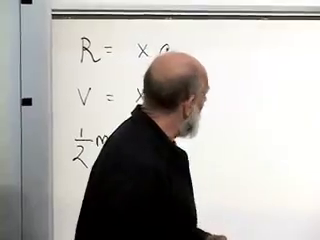
\includegraphics[width=0.72\textwidth]{lecture_09_figure_02.png}
  \caption{المترية المستوية المتمددّة، حيث يضرب عامل القياس عنصر الخط المكاني الإقليدي. إطار المصدر عند 00:09:12.}
  \label{fig:l09-expanding-metric-board}
\end{figure}

تخيل إحداثيات مرسومة على صفيحة مطاطية. تبقى علامات الإحداثيات مثبتة على الصفيحة بينما تنمو المسافة الفيزيائية بينها. وهكذا فإن فرقًا إحداثيًا مثل «من \(x=0\) إلى \(x=1\)» ليس إلا زوجًا من الوسوم. والمسافة التي يمثلها ذلك الفاصل هي \(a(t)\). ومسألة إيجاد المعادلة التي تحكم عامل القياس هذا هي المسألة الديناميكية في المحاضرة.

\section{الهندسات المكانية المغلقة والمستوية والمفتوحة}

الاستواء تبسيط رصدي، وليس نتيجة للتجانس. وهناك ثلاث هندسات مكانية متجانسة ومتساوية الخواص: ذات انحناء موجب، وصِفري، وسالب. ولفهم الحالة ذات الانحناء الموجب، يفيد أن نكون دقيقين بشأن البعد.

المكان الهندسي
\begin{equation}
  X_1^2+X_2^2=R^2
\end{equation}
هو دائرة، أي كرة أحادية \(S^1\). وداخلها الممتلئ قرص، ويُسمى أيضًا كرة ثنائية. وبإضافة إحداثي تضمين واحد نحصل على
\begin{equation}
  X_1^2+X_2^2+X_3^2=R^2,
\end{equation}
وهي الكرة الثنائية العادية \(S^2\). وبإضافة إحداثي تضمين رابع نحصل على
\begin{equation}
  X_1^2+X_2^2+X_3^2+X_4^2=R^2,
  \label{eq:l09-three-sphere}
\end{equation}
وهي كرة ثلاثية \(S^3\)، وهي نفسها فضاء ثلاثي الأبعاد. لا نستطيع تصور تضمينها رباعي الأبعاد، لكن الهندسة الجوهرية لا تحتاج إلى ذلك التضمين لكي توجد.

\begin{figure}[H]
  \centering
  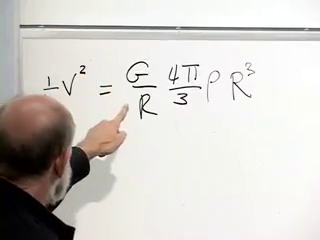
\includegraphics[width=0.72\textwidth]{lecture_09_figure_03.png}
  \caption{معادلة التضمين المستخدمة لتقديم الكرة الثلاثية. إطار المصدر عند 00:16:40.}
  \label{fig:l09-three-sphere-board}
\end{figure}

كل نقطة على كرة مثالية مكافئة هندسيًا لكل نقطة أخرى، وكل اتجاه عند نقطة ما مكافئ لأي اتجاه آخر. لذلك فالكرة متجانسة ومتساوية الخواص معًا. وإذا ضُرب نصف قطرها في \(a(t)\)، فإن الفضاء كله يتمدد أو ينكمش من دون تعيين مركز على الكرة. وإرجاع مثل هذا الكون إلى الماضي لا يضع كل المادة في موضع خاص واحد ضمن خلاء خارجي. بل إن الفضاء بأسره يصغر، فتغدو كل زوج من النقاط متقاربًا. والانفجار العظيم ليس انفجارًا من نقطة واحدة في الفضاء.

على كرة ذات انحناء موجب، يكون مجموع زوايا المثلثات الجيوديسية أكبر من \(180^\circ\). وفي المثلثات المستوية يكون مجموع الزوايا مساويًا تمامًا لـ \(180^\circ\). وفي هندسة متجانسة ذات انحناء سالب، تُمثَّل على نحو غير كامل بسطح سرجي، يكون مجموع الزوايا أقل من \(180^\circ\). وهذه الاختبارات الجوهرية تميّز بين الحالات الثلاث.

\begin{figure}[H]
  \centering
  \includegraphics[width=0.72\textwidth]{lecture_09_figure_07.png}
  \caption{الانحناء الموجب والصِفري والسالب موضحة عبر أشكالها المثلثية المميزة. إطار المصدر عند 00:37:30.}
  \label{fig:l09-curvature-board}
\end{figure}

إن متريةً محليةً مستويةً تمامًا لا تثبت بمفردها أن الفضاء غير منتهٍ طوبولوجيًا. فالطوبولوجيات المستوية المدمجة ممكنة رياضيًا، مع أن المحاضرة تعتمد أبسط نموذج إقليدي لا نهائي.
\editorialnote{هذا التحفظ المتعلق بالطوبولوجيا الشاملة غير مطلوب لأي من الديناميات المحلية اللاحقة.}

\section{الوسوم المواكبة للتمدد وقانون هابل}

لنعد الآن إلى الصفيحة المستوية المتمددة ونرسم عليها شبكة إحداثيات. في الإحداثيات المواكبة للتمدد، تتمدد الشبكة مع جريان المادة على المقاييس الكبيرة. وتحتفظ مجرة، أو على نحو أدق تجمّع من المجرات موصوف على نحو خشن بما يكفي، بوسم إحداثي ثابت تقريبًا، حتى مع تغيّر بعدها الفيزيائي عن جسم آخر مواكب للتمدد.

\begin{figure}[H]
  \centering
  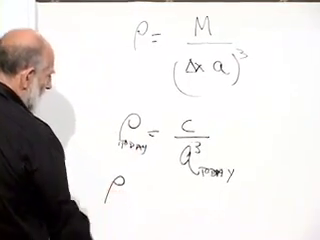
\includegraphics[width=0.72\textwidth]{lecture_09_figure_04.png}
  \caption{شبكة إحداثيات تُحمل مع صفيحة مكانية متمددة.
  إطار المصدر عند 00:22:20.}
  \label{fig:l09-comoving-grid-board}
\end{figure}

بالنسبة إلى جسمين يفصل بينهما على طول المحور \(x\) فاصل متواكب ثابت مقداره \(\Delta x\)، تكون المسافة الفيزيائية بينهما
\begin{equation}
  D(t)=a(t)\,\Delta x.
  \label{eq:l09-physical-distance}
\end{equation}
وباِشتقاق ذلك مع تثبيت \(\Delta x\) نحصل على
\begin{equation}
  v(t)=\dot a(t)\,\Delta x
      =\frac{\dot a(t)}{a(t)}D(t).
\end{equation}
وبتعريف
\begin{equation}
  H(t)\equiv\frac{\dot a(t)}{a(t)},
  \label{eq:l09-hubble-parameter}
\end{equation}
نحصل على قانون هابل،
\begin{equation}
  v=H(t)D.
  \label{eq:l09-hubble-law}
\end{equation}
إن كلمة «ثابت» في عبارة «ثابت هابل» تعني الثبات عبر الفضاء عند زمن كوني محدد. ولا تعني الثبات عبر التاريخ الكوني.

\begin{figure}[H]
  \centering
  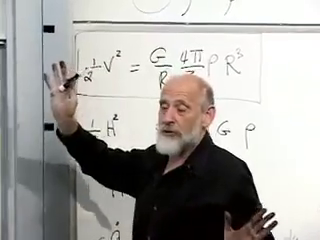
\includegraphics[width=0.72\textwidth]{lecture_09_figure_05.png}
  \caption{اشتقاق اللوح لـ \(D=a\Delta x\)،
  \(v=(\dot a/a)D=HD\). إطار المصدر عند 00:26:40.}
  \label{fig:l09-hubble-board}
\end{figure}

\begin{classroomqa}
\audiencequestion{إذا رأينا مجرة بعيدة كما كانت في زمن أبكر، فهل ينبغي حقًا أن يساوي معامل هابل المستنتج لها القيمة المقاسة في جوارنا اليوم؟}
\lecturerresponse{لا يكون ذلك إلا عندما يكون زمن النظر إلى الماضي صغيرًا مقارنة بعمر الكون. فعلى المسافات المعتدلة، يتغير \(H(t)\) تغيرًا طفيفًا بما يكفي لأن يكون عدد واحد مفيدًا. أمّا على المسافات الكونية حقًا، فإننا نرى حقبًا أبكر، ويجب تضمين الاعتماد الزمني لكل من \(a\) و\(H\). وذلك أحد الأسباب التي تجعلنا نحتاج إلى معادلة ديناميكية لعامل القياس.}
\end{classroomqa}

\section{الأشعة العدمية في نظام إحداثيات متمدد}

\begin{classroomqa}
\audiencequestion{هل يؤثر عامل القياس في انتشار الضوء بين المجرات البعيدة؟}
\lecturerresponse{يسلك شعاع الضوء مسارًا عدميًا، لذا \(d\tau=0\). وبالنسبة إلى شعاع يتحرك على طول المحور \(x\) الموجب، يكون \(dy=dz=0\)، وتعطي المترية المتمددة
\begin{align}
  0&=dt^2-a^2(t)dx^2,
  &dt&=a(t)dx,\notag\\
  &&\frac{dx}{dt}&=\frac{1}{a(t)}.
  \label{eq:l09-null-ray}
\end{align}
تتناقص السرعة الإحداثية كلما نما \(a(t)\)، لكن السرعة الفيزيائية المحلية للضوء تبقى \(c=1\). ويمثل فاصل إحداثي ثابت مسافة فيزيائية متزايدة.}
\end{classroomqa}

\begin{figure}[H]
  \centering
  \includegraphics[width=0.72\textwidth]{lecture_09_figure_06.png}
  \caption{الشرط العدمي و\(dt=a(t)dx\) لانتشار الضوء الشعاعي.
  إطار المصدر عند 00:30:54.}
  \label{fig:l09-null-board}
\end{figure}

يمكن اختيار إحداثيات يبدو فيها هذا الأمر نفسه بصيغة «يتباطأ الضوء كلما ازداد البعد»، لكن الأطوال والساعات تكتسب عندئذٍ أوصافًا مربكة بالمقدار المناظر. ولغة الفضاء المتمدد أنظف لأنها تحفظ العبارة المحلية القائلة إن كل راصد في سقوط حر يقيس السرعة نفسها للضوء.

\begin{classroomqa}
\audiencequestion{هل يوجد دليل على أن انتشار الضوء المحلي والفيزياء الذرية متماثلان في المجرات البعيدة؟}
\lecturerresponse{المقارنات اللابعدية وحدها ذات معنى إجرائي. اختر حجمًا ذريًا وحدةً للطول، وفترة ذرية أو نووية وحدةً للزمن، ثم اسأل كم عدد هذه الفترات الذي يحتاج إليه الضوء ليعبر الطول المختار. وتدعم الرصود الطيفية القول إن هذه النسب اللابعدية هي نفسها في المناطق البعيدة. والدليل غير مباشر، لكنه بالضبط نوع المقارنة الذي يُختبر به تماثل القوانين المحلية.}
\end{classroomqa}

عندما كان الكون المرصود صغيرًا للغاية، كان يمكن للضوء أن يعبر منطقة فيزيائية معيّنة بسرعة بحسب وحدة عبور الضوء الموافقة. وهذا لا يعني أن \(c\) كان مختلفًا. بل يعني أن المنطقة نفسها كانت صغيرة.

\section{كرة نيوتنية داخل الكون}

ننتقل الآن من الحركيات إلى الديناميكيات. لنضع أنفسنا عند الأصل ولنرسم كرة كبيرة بما يكفي لتحتوي كثيرًا من المجرات والعناقيد. اختر مجرة على حدّها. في كون متجانس يكون توزع الكتلة متناظرًا تناظرًا كرويًا حولنا، وتعطينا مبرهنة القشرة لنيوتن حقيقتين حاسمتين:
\begin{enumerate}
  \item كل مادة موزعة كرويًا خارج نصف القطر المختار تؤثر في المجرة الحدّية بقوة نيوتنية محصلة تساوي صفرًا؛
  \item كل المادة داخل الكرة تؤثر، في هذه الحركة الشعاعية، كما لو كانت متركزة في المركز.
\end{enumerate}
نستخدم إطارًا نكون فيه ساكنين، لذا تُقاس السرعات والتسارعات في الحجة التالية بالنسبة إلينا.

\begin{figure}[H]
  \centering
  \includegraphics[width=0.72\textwidth]{lecture_09_figure_08.png}
  \caption{بناء مبرهنة القشرة: نحن في المركز ومجرة اختبارية على حدّ كرة كبيرة متجانسة. إطار المصدر عند 00:41:10.}
  \label{fig:l09-shell-board}
\end{figure}

\begin{figure}[H]
  \centering
  \begin{tikzpicture}[scale=0.92,>=Latex]
    \draw[thick] (0,0) circle (2.35);
    \fill (0,0) circle (2pt) node[below left] {us};
    \fill (2.35,0) circle (2.2pt) node[right] {test galaxy \(m\)};
    \draw[->,thick,blue!65!black] (0.18,0) -- (2.15,0)
      node[midway,above] {\(R=a(t)x\)};
    \draw[->,thick,red!65!black] (2.35,0.12) -- (3.25,0.12)
      node[midway,above] {\(v=\dot a(t)x\)};
    \node[align=center,text width=7cm] at (0,-2.85)
      {outside shells cancel;\\enclosed mass acts at the center};
  \end{tikzpicture}
  \caption{إعادة بناء واضحة للبناء النيوتني.}
  \label{fig:l09-shell-clean}
\end{figure}

إذا كان للمجرة إحداثي مساير للتمدد ثابت هو \(x\)، فإن نصف قطرها الفيزيائي وسرعتها هما
\begin{equation}
  R(t)=x a(t),
  \qquad
  v(t)=x\dot a(t)=H(t)R(t).
  \label{eq:l09-radius-velocity}
\end{equation}
ولتكن \(M\) الكتلة المحصورة داخل الكرة و\(m\) كتلة مجرة الاختبار. عندئذ تكون الطاقة النيوتنية
\begin{equation}
  E=\frac12 m v^2-\frac{GMm}{R}.
  \label{eq:l09-newtonian-energy}
\end{equation}

\begin{figure}[H]
  \centering
  \includegraphics[width=0.72\textwidth]{lecture_09_figure_09.png}
  \caption{تسلسل اللوح الكامل لـ \(R=xa\) و\(v=x\dot a\)، ومعادلة الطاقة النيوتنية المخصَّصة للحالة \(E=0\). إطار المصدر عند 00:48:40.}
  \label{fig:l09-energy-board}
\end{figure}

قد تكون الطاقة موجبة أو صفرًا أو سالبة. لنبدأ عند الحد الفاصل بين الإفلات وإعادة الانهيار، \(E=0\)، الذي عنده
\begin{equation}
  \frac12 v^2=\frac{GM}{R}.
  \label{eq:l09-zero-energy}
\end{equation}

\begin{classroomqa}
\audiencequestion{ماذا تعني الطاقة الكلية الصفرية بالنسبة إلى المجرة المتباعدة؟}
\lecturerresponse{إنها بالضبط حالة سرعة الإفلات. فتعني الطاقة الموجبة حركة فوق سرعة الإفلات؛ وتعني الطاقة السالبة حركة دون سرعة الإفلات، وفي الصورة النيوتنية التي تحتوي على المادة فقط، عودة في نهاية المطاف. نبدأ عند الحد الفاصل بين هذين الاحتمالين، ثم نعود إلى الإشارتين الأخريين بعد اشتقاق معادلة الحالة المسطحة.}
\end{classroomqa}

\begin{classroomqa}
\audiencequestion{هل تتغير الكتلة المحصورة \(M\) مع تمدد الكرة؟}
\lecturerresponse{لا. الكرة مسايرة للتمدد، لذا تبقى الجسيمات نفسها داخلها. ينمو حجمها الفيزيائي وتنخفض كثافتها، لكن كتلتها الكلية المحصورة تبقى ثابتة. وهذا التمييز بين \(M\) و\(\rho(t)\) أساسي.}
\end{classroomqa}

لكثافة متجانسة \(\rho(t)\)،
\begin{equation}
  M=\frac{4\pi}{3}\rho(t)R^3.
  \label{eq:l09-enclosed-mass}
\end{equation}
وبالتعويض في \eqref{eq:l09-zero-energy} نحصل على
\begin{equation}
  \frac12 v^2
  =\frac{G}{R}\left(\frac{4\pi}{3}\rho R^3\right).
  \label{eq:l09-enclosed-energy}
\end{equation}

\begin{figure}[H]
  \centering
  \includegraphics[width=0.72\textwidth]{lecture_09_figure_10.png}
  \caption{تعويض الكتلة المحصورة في معادلة الطاقة الصفرية.
  إطار المصدر عند 00:54:16.060.}
  \label{fig:l09-enclosed-mass-board}
\end{figure}

باستخدام \(v=HR\)، نجد
\begin{align}
  \frac12 H^2R^2
    &=\frac{4\pi G}{3}\rho R^2,\\
  H^2
    &=\frac{8\pi G}{3}\rho.
\end{align}
ومن ثم فإن قانون التمدد للحالة ذات الطاقة الصفرية والمسطحة مكانيًا هو
\begin{equation}
  \boxed{\left(\frac{\dot a}{a}\right)^2
  =\frac{8\pi G}{3}\rho(t)}.
  \label{eq:l09-flat-friedmann}
\end{equation}
واختزال \(R^2\) ليس مصادفة. فلا بد لكون متجانس أن يعطي القيمة نفسها لـ \(H(t)\) أيًا كانت المجرة المسايرة للتمدد التي اختيرت بوصفها جسم الاختبار.

\begin{figure}[H]
  \centering
  \includegraphics[width=0.72\textwidth]{lecture_09_figure_11.png}
  \caption{اختزال نصف القطر وعلاقة فريدمان المسطحة الناتجة على اللوح. إطار المصدر عند 00:57:30.}
  \label{fig:l09-friedmann-board}
\end{figure}

\begin{classroomqa}
\audiencequestion{هل توجد أدلة على علاقة الطاقة الصفرية؟}
\lecturerresponse{يمكن استنتاج كلا الطرفين رصديًا: \(H\) من بيانات التباعد و\(\rho\) باحتساب النجوم والغاز والمادة المظلمة وطاقة الفراغ. وقد وجد القياس في زمن هذه المحاضرة أن الطرفين متسقان بدقة تقارب نسبة مئوية. وهذا القيد مهم: إذ يجب تضمين جميع أشكال الطاقة، كما أن مناقشة طاقة الفراغ اللاحقة تغيّر التأويل الساذج القائم على سرعة الإفلات.}
\end{classroomqa}

في الوحدات \(c=1\)، تكون لكثافة الكتلة وكثافة الطاقة الوحدات نفسها. ولذلك سيرمز الرمز \(\rho\) إلى كثافة الطاقة الكلية الملائمة للمكوّن الجاري بحثه.

\section{المادة العادية وقانون الثلثين}

لا تكون المعادلة \eqref{eq:l09-flat-friedmann} مغلقةً حتى نعرف كيف تتغير \(\rho(t)\). فلنملأ أولًا صندوقًا مستطيلًا مسايرًا للتمدد بجسيمات بطيئة الحركة وغير نسبية. أبعاده الإحداثية ثابتة، بينما ينمو حجمه الفيزيائي وفق
\begin{equation}
  V(t)=a^3(t)\,\Delta x\,\Delta y\,\Delta z.
\end{equation}
ويبقى عدد الجسيمات وكتلة السكون الكلية في الصندوق ثابتين، لذا
\begin{equation}
  \rho_{\mathrm m}(t)=\frac{C_{\mathrm m}}{a^3(t)}.
  \label{eq:l09-matter-dilution}
\end{equation}
وبالتطبيع إلى الحقبة الحالية \(t_0\)،
\begin{equation}
  \frac{\rho_{\mathrm m}(t)}{\rho_{\mathrm m,0}}
  =\left(\frac{a_0}{a(t)}\right)^3.
  \label{eq:l09-matter-normalized}
\end{equation}

\begin{figure}[H]
  \centering
  \includegraphics[width=0.72\textwidth]{lecture_09_figure_12.png}
  \caption{كثافة المادة، وتخففها وفق \(a^{-3}\)، وتطبيعها إلى القيمة الحالية. إطار المصدر عند 01:04:47.940.}
  \label{fig:l09-density-board}
\end{figure}

\begin{classroomqa}
\audiencequestion{ما القيمة التقريبية الحالية لكثافة طاقة الكون، وهل تستطيع الذرات العادية وحدها أن توفرها؟}
\lecturerresponse{إن إحصاء المادة الباريونية المرئية لا يعطي إلا جزءًا من الجواب. فلا بد أيضًا من تمثيل المادة المظلمة والطاقة المظلمة على هيئة كتلة-طاقة مكافئة. وتذكر المحاضرة مقياسًا تقريبيًا يتراوح من ذرة واحدة إلى بضع عشرات من مكافئات كتلة الهيدروجين في كل متر مكعب، مع التأكيد على رتبة المقدار لا على جرد دقيق.}
\end{classroomqa}

أدخل \eqref{eq:l09-matter-dilution} في
\eqref{eq:l09-flat-friedmann} واجمع جميع العوامل المستقلة عن الزمن في ثابت موجب \(C\):
\begin{equation}
  \left(\frac{\dot a}{a}\right)^2=\frac{C}{a^3},
  \qquad
  \dot a^2=\frac{C}{a}.
  \label{eq:l09-matter-ode}
\end{equation}
وهناك طريقتان واضحتان لحلها. إن تجربة حل بقانون قوى
\(a=K t^p\) تقتضي
\begin{equation}
  p-1=-\frac{p}{2},
  \qquad p=\frac23.
\end{equation}
وبصورة مكافئة، خذ فرع الجذر التربيعي الموافق للتمدد وأجرِ التكامل:
\begin{equation}
  a^{1/2}\frac{da}{dt}=\sqrt C,
  \qquad
  \int a^{1/2}da=\sqrt C\int dt,
\end{equation}
ومن ثم، بعد اختيار الانفجار العظيم مبدأً للزمن،
\begin{equation}
  a^{3/2}\propto t,
  \qquad
  \boxed{a(t)\propto t^{2/3}}.
  \label{eq:l09-matter-solution}
\end{equation}
يفقد الاشتقاق المباشر عاملًا لفترة وجيزة أثناء مطابقة المعاملات، ثم يعود إلى التكامل ويتحقق من الأسّ. وتُبقي الملاحظات على هذا التحقق، لكنها تعرض الجبر المصحح فقط.

\begin{figure}[H]
  \centering
  \includegraphics[width=0.72\textwidth]{lecture_09_figure_13.png}
  \caption{محاولة قانون القوى والأسّ المؤطَّر \(p=2/3\). إطار المصدر
  عند 01:13:05.}
  \label{fig:l09-matter-solution-board}
\end{figure}

باشتقاق الحل نحصل على
\begin{equation}
  H(t)=\frac{\dot a}{a}=\frac{2}{3t}.
  \label{eq:l09-matter-hubble}
\end{equation}
وكان معامل هابل أكبر في الماضي. ولذلك، عند النظر إلى مسافات بعيدة بما يكفي بحيث نرى زمنًا معتبرًا للنظر إلى الماضي، لا ينبغي تمديد العلاقة الخطية المحلية باستخدام \(H_0\) الحالي من دون تغيير.

\begin{figure}[H]
  \centering
  \includegraphics[width=0.72\textwidth]{lecture_09_figure_14.png}
  \caption{حساب \(\dot a/a\) عندما يكون \(a\propto t^{2/3}\) يعطي
  \(H=2/(3t)\). إطار المصدر عند 01:20:42.}
  \label{fig:l09-hubble-time-board}
\end{figure}

\section{إشارة الطاقة والانحناء المكاني}

قادنا الاستدلال النيوتني إلى الحالة المسطحة ذات الطاقة الصفرية. وتضيف النسبية العامة حقيقة لا يمكن الحصول عليها من مبرهنة القشرة وحدها: فإشارة الطاقة النوعية على النمط النيوتني تقابل إشارة الانحناء المكاني.
\begin{center}
\begin{tabular}{@{}>{\raggedright\arraybackslash}p{0.20\linewidth}
                    >{\raggedright\arraybackslash}p{0.29\linewidth}
                    >{\raggedright\arraybackslash}p{0.37\linewidth}@{}}
  \toprule
  الطاقة الكلية & الانحناء المكاني & المصير في نموذج المادة فقط \\
  \midrule
  موجبة & سالب (مفتوح) & يتمدد إلى الأبد \\
  صفرية & صفري (مسطّح) & يقترب من حد الإفلات \\
  سالبة & موجب (مغلق) & يتمدد، ثم ينعطف، ثم ينهار من جديد \\
  \bottomrule
\end{tabular}
\end{center}
ويفترض العمود الأخير عدم وجود طاقة فراغ. وفي تشبيه المقذوفات، تعني الطاقة الموجبة أن الحركة فوق سرعة الإفلات، وتعني الطاقة الصفرية أنها عند سرعة الإفلات تمامًا، وتعني الطاقة السالبة أنها دون سرعة الإفلات. وتطابق معادلات أينشتاين هذه الحالات الثلاث مع الهندسة المكانية المفتوحة والمسطحة والمغلقة، على الترتيب.

\section{الفوتونات وقانون النصف}

يفترض قانون المادة \(\rho\propto a^{-3}\) أن طاقة كل جسيم ثابتة تقريبًا بينما تنخفض الكثافة العددية. وتخالف الفوتونات هذا الافتراض. فبالنسبة إلى فوتون،
\begin{equation}
  E=h\nu=\frac{hc}{\lambda}.
\end{equation}
يمدّ التمدد طول موجته بنسبة تتناسب مع عامل القياس،
\begin{equation}
  \lambda\propto a,
  \qquad E\propto a^{-1}.
\end{equation}
ولا تزال الكثافة العددية للفوتونات تنخفض كما \(a^{-3}\)، وتضيف طاقة كل فوتون عاملًا إضافيًا مقداره \(a^{-1}\). لذلك
\begin{equation}
  \boxed{\rho_{\mathrm r}(t)\propto a^{-4}(t)}.
  \label{eq:l09-radiation-dilution}
\end{equation}

يجسد تشبيه وتر الغيتار الصورة الفيزيائية. انقر وترًا ثم أطِل جزأه المهتز: يزداد الطول الموجي وتنخفض النغمة. ويتصرف نمط فوتوني في صندوق مساير للتمدد آخذ في التوسع على نحو مشابه. وإذا عكسنا الصورة، فإن الانضغاط يقصر الأطوال الموجية ويرفع طاقات الفوتونات.

\begin{figure}[H]
  \centering
  \includegraphics[width=0.72\textwidth]{lecture_09_figure_15.png}
  \caption{علاقة كثافة المادة بعد تمديدها على اللوح لتشمل قانون تحجيم الإشعاع \(\rho_{\mathrm r}\propto a^{-4}\). إطار المصدر عند 01:29:20.}
  \label{fig:l09-radiation-board}
\end{figure}

يؤدي استخدام \(\rho_{\mathrm r}\propto a^{-4}\) في معادلة فريدمان المستوية إلى
\begin{equation}
  \left(\frac{\dot a}{a}\right)^2=\frac{C_{\mathrm r}}{a^4},
  \qquad
  \dot a\propto a^{-1},
\end{equation}
ومن ثم
\begin{equation}
  \boxed{a(t)\propto t^{1/2}}.
  \label{eq:l09-radiation-solution}
\end{equation}
وهذا ينمو أبطأ من \(t^{2/3}\). وإذا عدنا بعيدًا بما يكفي إلى الماضي، فلا بد أن يهيمن الإشعاع على المادة العادية لأن \(a^{-4}\) يزداد أسرع من \(a^{-3}\) كلما تناقص \(a\). وتضع المحاضرة مرحلة تعادل المادة والإشعاع تقريبًا عند الحقبة التي كان فيها عامل القياس أصغر بنحو ألف مرة مما هو عليه اليوم. وقبل تلك المرحلة كان الكون خاضعًا لهيمنة الإشعاع؛ وبعدها كان، طوال فترة طويلة، خاضعًا لهيمنة المادة.

\section{طاقة الفراغ والتمدد الأسي}

لطاقة الفراغ سلوك معاكس فيما يتعلق بالاعتماد على عامل القياس. فكثافتها خاصية للفضاء الخالي، ولا تتناقص مع تمدد الكون:
\begin{equation}
  \rho_\Lambda=\text{constant}.
  \label{eq:l09-vacuum-density}
\end{equation}
وتصبح المادة العادية والإشعاع أكثف كلما اتجهنا نحو الماضي، بينما لا ينطبق ذلك على هذا الحد. ولذلك كانت أقل أهمية في الكون المبكر، وتصبح أكثر أهمية كلما تخلخلت المكونات الأخرى. وتستعمل المحاضرة التقدير السائد آنذاك، ومفاده أن طاقة الفراغ تسهم بنحو \(70\%\) من كثافة الطاقة الكونية اليوم.

مع ثبات \(\rho_\Lambda\)، تعطي المعادلة \eqref{eq:l09-flat-friedmann} معدل تمدد ثابتًا
\begin{equation}
  H_\Lambda=\sqrt{\frac{8\pi G}{3}\rho_\Lambda},
  \qquad
  \frac{\dot a}{a}=H_\Lambda.
\end{equation}
ولذلك
\begin{equation}
  \boxed{a(t)=a(t_i)e^{H_\Lambda(t-t_i)}}.
  \label{eq:l09-vacuum-solution}
\end{equation}

\begin{figure}[H]
  \centering
  \includegraphics[width=0.72\textwidth]{lecture_09_figure_16.png}
  \caption{معادلة الكثافة الثابتة التي تؤدي إلى تمدد أسي.
  إطار المصدر عند 01:35:48.}
  \label{fig:l09-vacuum-board}
\end{figure}

على المقياس المرصود المذكور في المحاضرة، يتضاعف البعد الخطي للكون خلال نحو عشرة إلى اثني عشر مليار سنة. ولا يزال أصل كثافة الفراغ الصغيرة هذه، ولكن غير المنعدمة، غير مفسَّر؛ أما وجودها وتأثيرها في التمدد فهما حقيقتان تجريبيتان.

\begin{classroomqa}
\audiencequestion{هل طاقة الفراغ هي نفسها الطاقة المظلمة في هذا النقاش؟}
\lecturerresponse{نعم. تدل «الطاقة المظلمة» هنا على كثافة ثابتة لطاقة الفراغ، أي ما يكافئ ثابتًا كونيًا. ويمكن تصوّر نماذج أكثر عمومية للطاقة المظلمة تعتمد على الزمن، لكنها ليست جزءًا من حساب هذه المحاضرة.}
\end{classroomqa}

\section{كيف يسبّب الكون المتمدد انزياح الضوء نحو الأحمر}

\begin{classroomqa}
\audiencequestion{كيف يمكن للفوتونات أن تعرف أننا اخترنا إحداثيات مسايرة للتمدّد، ومن ثم تخفض طاقتها؟}
\lecturerresponse{هي لا تستجيب لتسمياتنا. بل تنتشر خلال هندسة تتغير فيها المسافات الفيزيائية. والقطار الموجي الذي يشغل منطقة يتضاعف حجمها الفيزيائي يكتسب طولًا موجيًا متضاعفًا. أما الإحداثيات المسايرة فمجرد وسيلة تصف هذا التمطط بصورة مقتصدة؛ وهي لا تسببه.}
\end{classroomqa}

\begin{classroomqa}
\audiencequestion{من أين تأتي فوتونات الخلفية التي تصل إلينا اليوم؟}
\lecturerresponse{إن النظر إلى مسافات أبعد يعني النظر إلى أزمنة أبكر. وفي نهاية المطاف نرى الحقبة التي كانت فيها مادة الكون بلازما متأينة، معتمة لأن الفوتونات كانت تتبعثر مرارًا عن الجسيمات الحرة المشحونة. ويظهر الحد الذي استطاعت الفوتونات بعده أن تسافر إلينا بحرية للمرة الأخيرة على هيئة كرة تحيط بالراصد: سطح التبعثر الأخير.}
\end{classroomqa}

\begin{figure}[H]
  \centering
  \includegraphics[width=0.72\textwidth]{lecture_09_figure_17.png}
  \caption{الرسم التخطيطي المتمركز على الراصد لسطح التبعثر الأخير والأغلفة المتزايدة بُعدًا.
  إطار المصدر عند 01:42:05.}
  \label{fig:l09-last-scattering-board}
\end{figure}

\begin{figure}[H]
  \centering
  \begin{tikzpicture}[scale=0.9,>=Latex]
    \fill (0,0) circle (2pt) node[below] {observer};
    \draw[thick,orange!70!black] (0,0) circle (2.55);
    \node[orange!70!black,align=center] at (0,3.05)
      {surface of last scattering};
    \foreach \a in {25,75,145,210,285,335}{
      \draw[->,blue!60!black] ({2.55*cos(\a)},{2.55*sin(\a)}) --
        ({1.7*cos(\a)},{1.7*sin(\a)});
    }
    \draw[decorate,decoration={snake,amplitude=1.5pt,segment length=7pt},
      red!65!black,thick,->] (-2.5,0) -- (-0.15,0);
    \node[red!65!black,below] at (-1.35,-0.15)
      {redshifted photon};
  \end{tikzpicture}
  \caption{إعادة بناء منقّحة لصورة التبعثر الأخير.}
  \label{fig:l09-last-scattering-clean}
\end{figure}

انبعث الإشعاع بطيف مميز لبلازما حارة، ويصل إلينا بأطوال موجية أطول بنحو ألف مرة. وبلغة دوبلر المستعملة في المحاضرة، يبتعد السطح الباعث البعيد بسرعة، ويكون إشعاعه منزاحًا بشدة نحو الأحمر. وباللغة الهندسية، تُمطّ الموجة أثناء انتشارها. وكلتا الصورتين تعبّران عن العلاقة نفسها،
\begin{equation}
  1+z=\frac{\lambda_0}{\lambda_{\mathrm{em}}}
      =\frac{a_0}{a_{\mathrm{em}}}.
  \label{eq:l09-cosmological-redshift}
\end{equation}
\editorialnote{تمثل المعادلة \eqref{eq:l09-cosmological-redshift} الصيغة الكمية المعيارية لوصفي الاستطالة ودوبلر في المحاضرة.}

في حقبة رصد أبكر، لكانت كرة التبعثر الأخير أقرب في الصورة المناظرة، ولكانت فوتونات الخلفية المرصودة أقل انزياحًا نحو الأحمر، ومن ثم أعلى طاقة. ومع تقدم الزمن الكوني، تكون للفوتونات التي تصل إلى راصد مساير للتمدّد من تلك البلازما المبكرة أطوال موجية تزداد طولًا تدريجيًا.

\section{إلى أين تذهب طاقة الفوتون المنزاح نحو الأحمر؟}

\begin{classroomqa}
\audiencequestion{يُصدر فوتون بطاقة \(h\nu_{\mathrm{em}}\) ثم يصل منزاحًا نحو الأحمر بطاقة أقل. ماذا حدث للفارق؟}
\lecturerresponse{بدأ الاشتقاق النيوتني في الأصل بوصفه معادلة طاقة. وصيغته الكونية تربط معدل التمدد بكثافة طاقة المحتوى المادي، لذلك لا يمكن التعامل مع طاقة المادة والتمدد على أنهما حسابان محفوظان على نحو منفصل. وتصف المحاضرة طاقة الفوتون المفقودة بأنها تدخل في المحاسبة الحركية للتمدد. ويجعل تشبيه مكبس مملوء بالإشعاع ذلك محسوسًا: فضغط الإشعاع يدفع المكبس إلى الخارج، وتزداد الأطوال الموجية للفوتونات، وتصبح طاقتها المفقودة شغلًا ميكانيكيًا وطاقة حركية للمكبس.}
\end{classroomqa}

\begin{figure}[H]
  \centering
  \includegraphics[width=0.72\textwidth]{lecture_09_figure_18.png}
  \caption{تُظهر اللوحة معادلة الطاقة النيوتنية المؤطَّرة فوق معادلة فريدمان المناظرة.
  إطار المصدر عند 01:44:42.}
  \label{fig:l09-energy-bookkeeping-board}
\end{figure}

\begin{classroomqa}
\audiencequestion{ما الذي يربط طاقة الإشعاع بالتمدد؟}
\lecturerresponse{الضغط. ففي أسطوانة ذات مكبس متحرك، تنقل الفوتونات زخمًا إلى الجدار. ومع تحرك المكبس، يبذل الإشعاع شغلًا؛ فتزداد أطوالها الموجية وتنخفض طاقتها. وليس في الكون المتجانس المتمدد مكبس خارجي حرفي، لكن تشبيه \(p\,dV\) يوضح لماذا تنخفض كثافة طاقة الإشعاع أسرع مما يفسره تخفف العدد وحده.}
\end{classroomqa}

\begin{figure}[H]
  \centering
  \includegraphics[width=0.72\textwidth]{lecture_09_figure_19.png}
  \caption{المكبس المتحرك المملوء بالفوتونات والمستخدَم لتصوير شغل الضغط.
  إطار المصدر عند 01:46:40.}
  \label{fig:l09-piston-board}
\end{figure}

\begin{figure}[H]
  \centering
  \begin{tikzpicture}[scale=0.92,>=Latex]
    \draw[thick] (0,0) rectangle (5.3,2.6);
    \draw[very thick] (4.25,0) -- (4.25,2.6);
    \draw[very thick] (4.25,1.3) -- (5.25,1.3);
    \draw[->,thick,red!65!black] (5.25,1.3) -- (6.2,1.3)
      node[right] {moving piston};
    \foreach \y in {0.55,1.3,2.05}{
      \draw[decorate,decoration={snake,amplitude=1.4pt,segment length=6pt},
        blue!65!black,->] (0.35,\y) -- (3.9,\y);
    }
    \node at (2.15,-0.45) {radiation does \(p\,dV\) work};
  \end{tikzpicture}
  \caption{إعادة بناء منقّحة لتشبيه الإشعاع والمكبس.}
  \label{fig:l09-piston-clean}
\end{figure}

تتطلب الطاقة في النسبية العامة قدرًا من الحذر. ففي زمكان متمدد عام، قد لا توجد طاقة كلية محفوظة وحيدة مماثلة لطاقة نظام نيوتني معزول. ومع ذلك يبقى انحفاظ موتر الإجهاد-الطاقة موضعيًا ساريًا، وبالنسبة إلى مائع متجانس فإنه يعطي معادلة الاستمرارية
\begin{equation}
  \dot\rho+3H(\rho+p)=0,
  \label{eq:l09-continuity}
\end{equation}
التي تتضمن حد شغل الضغط الكامن وراء قوانين تدرج المادة والإشعاع.\editorialnote{تمثل المعادلة \eqref{eq:l09-continuity} الصياغة الموضعية الدقيقة في النسبية العامة التي تقوم عليها محاكاة المحاضرة المتعمدة للمحاسبة النيوتنية للطاقة.}

تجعل طاقة الفراغ هذا اللغز أشد حدة على نحو خاص. فبما أن كثافتها تبقى ثابتة بينما يزداد الحجم، فإن طاقة الفراغ الكلية في منطقة مسايرة للتمدّد تزداد. وضغطها السالب جزء من المصدر الثقالي، وهو يدفع التمدد المتسارع. لذلك لا ينبغي المطالبة بانحفاظ منفصل لما يُسمى بسذاجة «طاقة المادة في صندوق مساير للتمدّد» من دون إدخال الهندسة وشغل الضغط.

\section{لماذا يمكن إزالة عامل القياس من الحد الزمني}

\begin{classroomqa}
\audiencequestion{لماذا يضرب عامل القياس الجزء المكاني من المترية لا الجزء الزمني؟}
\lecturerresponse{ذلك اختيار لإحداثي الزمن. افترض أننا نبدأ بإحداثي الزمن المطابق \(t\) بحيث
\begin{equation}
  d\tau^2=A^2(t)\left(dt^2-dx^2\right).
\end{equation}
وعرّف زمنًا كونيًا جديدًا \(T\) بالعلاقة
\begin{equation}
  dT=A(t)\,dt.
\end{equation}
فعندئذ
\begin{equation}
  d\tau^2=dT^2-A^2\bigl(t(T)\bigr)dx^2.
\end{equation}
يكون العامل المشترك أمام تفاضل الزمن قد اختفى، بينما يبقى عامل القياس الفيزيائي في الحد المكاني.}
\end{classroomqa}

\begin{figure}[H]
  \centering
  \includegraphics[width=0.72\textwidth]{lecture_09_figure_20.png}
  \caption{إعادة تعريف الزمن \(dT=A(t)dt\) التي تحوّل الزمن المطابق إلى زمن كوني.
  إطار المصدر عند 01:51:05.}
  \label{fig:l09-time-reparam-board}
\end{figure}

\section{الانحناء وطاقة الفراغ والمصير الكوني}

\begin{classroomqa}
\audiencequestion{إذا كان الكون ذا انحناء موجب، أفلا ينبغي أن نرى المجرات آتية نحونا بالفعل؟}
\lecturerresponse{ليس بالضرورة. فالمقذوف الذي يُطلَق بسرعة دون سرعة الإفلات يسير أولًا إلى الخارج، ويبلغ نقطة انقلاب، ثم لا يعود ساقطًا إلا لاحقًا. ونحن نرصد الكون خلال طور تمدد. ومن دون طاقة فراغ، فإن كونًا ماديًا ذا انحناء موجب سينكمش من جديد في نهاية المطاف. أما طاقة فراغ موجبة وكبيرة بما يكفي فتمنع ذلك الانعطاف، وتبدو القيمة المرصودة كبيرة بما يكفي لجعل التمدد الطويل الأمد أسيًا بصرف النظر عن انحناء مكاني صغير.}
\end{classroomqa}

ليس المستقبل الأسي فردوسًا طاقيًا. فالنجوم تنطفئ في نهاية المطاف، وتنخفض كثافتا المادة والإشعاع أسيًا، وتنتقل المناطق البعيدة إلى ما وراء الاتصال السببي. وتبقى طاقة الفراغ، بينما تصبح البنى العادية أبرد تدريجيًا وأكثر تخلخلًا.

\begin{classroomqa}
\audiencequestion{إذا عدنا أبعد إلى الماضي، فهل يكون عدد الفوتونات أكبر من عدد الجسيمات العادية؟}
\lecturerresponse{إن نسبة عدد الفوتونات إلى عدد الباريونات هائلة بالفعل، وتقارب \(10^{10}\) فوتونًا لكل باريون في تقدير المحاضرة، ويظل كلٌّ منهما، ضمن حجم مواكب للتمدد، ثابتًا تقريبًا. وما يتغير كلما اتجهنا نحو الماضي هو أساسًا الطاقة لكل فوتون. وترتفع طاقات الفوتونات على نحو \(a^{-1}\)، في حين أن كتل السكون غير النسبية لا تزداد. لذلك يهيمن الإشعاع على كثافة الطاقة في الأزمنة المبكرة، مع أن نسبة العدد نفسها لا يلزم أن تتغير.}
\end{classroomqa}

الدرس المركزي هو أن الهندسة وحدها لا تحدد التاريخ الكوني. فمعادلة فريدمان المسطحة توفّر العلاقة بين التمدد وكثافة الطاقة، لكن المحتوى المادي هو الذي يحدد الاعتماد على الزمن. فالمادة غير النسبية تعطي \(a\propto t^{2/3}\)، والإشعاع يعطي \(a\propto t^{1/2}\)، وطاقة الفراغ الثابتة تعطي تمددًا أسيًا. وهذه القوانين الثلاثة تنظّم العصور المتعاقبة للكون وتفسّر لماذا يتحكم عامل القياس نفسه في المسافات، والانزياحات نحو الأحمر، ومعامل هابل المتغيّر.

\end{document}